\documentclass[conference]{IEEEtran}
\IEEEoverridecommandlockouts
% The preceding line is only needed to identify funding in the first footnote. If that is unneeded, please comment it out.
% \usepackage{cite}
% \usepackage{amsmath,amssymb,amsfonts}
% \usepackage{algorithmic}
% \usepackage{graphicx}
% \usepackage{textcomp}
% \usepackage{xcolor}
\def\BibTeX{{\rm B\kern-.05em{\sc i\kern-.025em b}\kern-.08em
    T\kern-.1667em\lower.7ex\hbox{E}\kern-.125emX}}

% !TEX root =  ../paper.tex

\usepackage{url}

\usepackage{graphicx}
\usepackage{diagbox}
%\usepackage{time}

%\usepackage[noadjust]{cite} % Sort all citations
%\usepackage[sort&compress,numbers]{natbib}     % Sort all citations

\usepackage{xspace}
\usepackage{xcolor} % Used to highlight comments
\usepackage{tabularx}
% \usepackage{subfig}
%flushend – Balancing columns at last page
% \usepackage[font=normalsize]{caption}
%\usepackage{msc}
% \usepackage[keeplastbox]{flushend}
% \usepackage[group-separator={,}, mode=text, math-rm=\text, detect-all, binary-units=true, per-mode=symbol, range-phrase={\,--\,}, range-units=single]{siunitx}
% \usepackage{enumitem}
\usepackage[T1]{fontenc}
\usepackage{hyperref}
% \usepackage[hyphens]{url}
\usepackage{amsmath}
\usepackage{mathtools}
\usepackage{tikz}
\usepackage{soul}
\usepackage{multirow}
\usepackage{booktabs}
\usepackage{csquotes} % Used for easy quotation marks
\usepackage[normalem]{ulem} % For strike-through text
\usepackage[capitalize,noabbrev]{cleveref}

% code snippet
\usepackage{listings}
% appendix
% \usepackage{appendix}
% proper typesetting of units
\usepackage{siunitx} 
% landscape
\usepackage{pdflscape}

% reduce virtical space b/w paragraphs and subequations
\usepackage{etoolbox}
\preto\subequations{\ifhmode\unskip\fi}

%Floatbarrier
\usepackage{placeins}

%Used to handle acronyms
\usepackage[printonlyused, footnote ]{acronym}

%Side by side figures
%\usepackage[demo]{graphicx}
\usepackage{caption}
\usepackage{subcaption}

% !TEX root =  ../paper.tex

% common acronyms
\newcommand{\etal}{{et~al}.\@~}
\newcommand{\eg}{e.g.,\xspace}
\newcommand{\ie}{i.e.,\xspace}
\newcommand{\etc}{etc.\xspace}

% % typographic macros
% \newcommand{\hex}[1]{\ensuremath{\texttt{0x#1}}}
% \SetEnumitemKey{myindent}{labelindent=\parindent, itemindent=*, leftmargin=2\parindent}
\newcommand{\var}[1]{\ensuremath{\mathit{#1}}}
\newcommand{\conc}{\ensuremath{\;\vert\;}}
\newcommand{\func}[1]{\texttt{#1}}

% Author-specific Comments
\newcommand{\todo}[1]{\FloatBarrier\textcolor{red}{\textbf{TODO:} #1}\FloatBarrier}

% For tables
\usepackage{booktabs}
\newcommand{\ra}[1]{\renewcommand{\arraystretch}{#1}}
\usepackage{longtable}

% \newcommand{\mk}[1]{\hl{#1}}  % Mark for the changes
\newcommand{\mk}{}  % Mark for the changes

% \newcommand{\ad}[1]{\textcolor{red}{#1}}
\newcommand{\ad}[1]{#1}
% \newcommand{\ad}[1]{\colorbox{green}{#1}}


\usepackage[symbol]{footmisc}
\renewcommand{\thefootnote}{\fnsymbol{footnote}}


% Url style in references same as the other text
% \urlstyle{same}

% \setlist[itemize]{leftmargin=1em, itemsep=-0.1em, itemindent=0em}
% \setlist[enumerate]{leftmargin=1.2em, itemindent=0em, itemsep=-0.1em}

\def\sectionautorefname{Section}
\let\subsectionautorefname\sectionautorefname
\let\subsubsectionautorefname\sectionautorefname

\renewcommand{\paragraph}[1]{\noindent\textbf{#1.}}
\newcommand{\subparagraph}[1]{\noindent$\bullet$\textit{~#1:}}

\newcommand*\circled[1]{\tikz[baseline=(char.base)]{
            \node[shape=circle,fill,inner sep=1.5pt] (char) {\textcolor{white}{#1}};}}

\newcommand*\tcircled[1]{\tikz[baseline=(char.base)]{
            \node[shape=circle,draw,fill=none,inner sep=0.5pt] (char) {\textcolor{black}{#1}};}}

\newcounter{lineno}
\DeclareRobustCommand{\line}[1]{%
    \refstepcounter{lineno}%
    \hfill{\normalsize \circled{\small \thelineno}}\label{#1}
}

\newcommand{\stepnumber}[1]{\tikz[baseline=(char.base)]{
	\node[shape=circle, draw, thick, inner sep=.5pt] (char) {\small\sffamily\bfseries #1}
}}

% \newcolumntype{C}[1]{>{\centering\let\newline\\\arraybackslash\hspace{0pt}}m{#1}}

\newcommand{\mac}[1]{\ensuremath{\mathsf{MAC}_{#1}}}

\newcounter{protocol}

\PassOptionsToPackage{hyphens}{url}

\setlength\belowcaptionskip{-1ex}

\definecolor{codegreen}{rgb}{0,0.6,0}
\definecolor{codegray}{rgb}{0.5,0.5,0.5}
\definecolor{codepurple}{rgb}{0.58,0,0.82}
\definecolor{backcolour}{rgb}{0.95,0.95,0.92}

\lstdefinestyle{mystyle}{
    backgroundcolor=\color{backcolour},   
    commentstyle=\color{codegreen},
    keywordstyle=\color{magenta},
    keywordstyle=[1]\color{magenta},
    numberstyle=\tiny\color{codegray},
    stringstyle=\color{codepurple},
    basicstyle=\ttfamily\footnotesize,
    breakatwhitespace=false,         
    breaklines=true,                 
    captionpos=b,                    
    keepspaces=true,                 
    numbers=left,                    
    numbersep=5pt,                  
    showspaces=false,                
    showstringspaces=false,
    showtabs=false,                  
    tabsize=2,
    otherkeywords = {DISTINCT, WITH, REFERENCES, TEXT, AUTOINCREMENT},
}

\lstset{style=mystyle}

\catcode`_=12 %
\renewcommand{\texttt}[1]{%
  \begingroup
  \ttfamily
  \begingroup\lccode`~=`/\lowercase{\endgroup\def~}{/\discretionary{}{}{}}%
  \begingroup\lccode`~=`[\lowercase{\endgroup\def~}{[\discretionary{}{}{}}%
  \begingroup\lccode`~=`.\lowercase{\endgroup\def~}{.\discretionary{}{}{}}%
  \begingroup\lccode`~=`_\lowercase{\endgroup\def~}{_\discretionary{}{}{}}%
  \catcode`/=\active\catcode`[=\active\catcode`.=\active\catcode`_=\active
  \scantokens{#1\noexpand}%
  \endgroup
}
\catcode`_=8 % 





%% Some more packages that you may want to use.  Have a look at the
%% file, and consult the package docs for each.
% \input{setup/extrapackages}

%% Our layout configuration.  DO NOT CHANGE.
% \input{setup/layoutsetup}

%% Theorem environments.  You will have to adapt this for a German
%% thesis.
% \input{setup/theoremsetup}

%% Helpful macros.
% \input{setup/macrosetup}


\begin{document}


\title{Network Zoning in Data Centers
% *\\
% {\footnotesize \textsuperscript{*}Note: Sub-titles are not captured in Xplore and
% should not be used}
% \thanks{Identify applicable funding agency here. If none, delete this.}
}

\author{
    \IEEEauthorblockN{Manuel Meinen}
        \IEEEauthorblockA{
            % \textit{dept. name of organization (of Aff.)} \\
            \textit{ETH Z{\"u}rich} \\
            % \textit{name of organization (of Aff.)}\\
            % City, Country \\
            mmeinen@student.ethz.ch}
    \and
    \IEEEauthorblockN{Jonghoon Kwon}
        \IEEEauthorblockA{
            % \textit{dept. name of organization (of Aff.)} \\
            \textit{ETH Z{\"u}rich} \\
            % City, Country \\
            jong.kwon@inf.ethz.ch}
    \and
    \IEEEauthorblockN{Claude H{\"a}hni}
        \IEEEauthorblockA{
            % \textit{dept. name of organization (of Aff.)} \\
            \textit{ETH Z{\"u}rich} \\
            % City, Country \\
            claude.haehni@inf.ethz.ch}
    \and
    \IEEEauthorblockN{Adrian Perrig}
        \IEEEauthorblockA{
            % \textit{dept. name of organization (of Aff.)} \\
            \textit{ETH Z{\"u}rich} \\
            % City, Country \\
            adrian.perrig@inf.ethz.ch}
}

\maketitle

\begin{abstract}
 Network zoning is an important way of securing assets in a network. The process of creating and managing network zones, as well as transitions between these zones has historically been proven to be hard. Especially in data centers of large cloud providers, network zoning is extremely important, since it is a multi-tenancy environment. The new inter-domain network zoning architecture named MONDRIAN simplifies the management of network zones and transitions between them. However, it is designed to be used in corporate networks, meaning that it’s not applicable to data center networks. 

 %Methods
 %  - Design, implement and evaluate a PoC
 
 In this thesis we redesigned MONDRIAN to be usable and beneficial in the context of data center network security. We created a \acl{PoC} implementation, which leverages the logically centralized property of MONDRIAN while being optimized for large scale data centers. We rigorously evaluated the functionality, security and performance of the newly designed MONDRIAN variant.

 %Results
 %  - Functionality achieved, Security as on the same level as original MONDRIAN and performance ok for PoC implementation. Scalability and integrates well in DCs

 The results show that with the new design, we achieve the full functionality of MONDRIAN and are therefore able to provide equally strong security and manageability benefits. The performance is on a decent level for a \acl{PoC} implementation and scalability is shown in several experiments.
 
 %Conclusion
 %  - MONDRIAN is feasible in the context of DCs thanks to the new design
 %  - Clear benefits exist
 The thesis shows the feasibility of employing a logically centralized network zoning architecture like MONDRIAN in the context of data center networking. It proposes a completely redesigned architecture, which is optimized for the use in modern data centers and provides data center operators with the benefits MONDRIAN has to offer.
\end{abstract}

\begin{IEEEkeywords}
component, formatting, style, styling, insert
\end{IEEEkeywords}

\section{Introduction}
\label{sec:introduction}
% \chapter{Introduction}
%Motivation
Network zoning in data centers of course already exists today. However, current approaches require us to configure multiple components such as routers, firewalls and \acsp{VPN} (\aclp{VPN}). Some of these configurations are site specific, while others need to be consistent across sites. This combined with the fact that there is typically no central database containing all the zone transition polices makes the management of network zones in data centers extremely difficult. %Data center operators usually need to decide if they want to sacrifice either \textbf{functionality} by not allowing zone transitions at all, \textbf{flexibility} by not moving hosts around and not changing once established zone transition policies or \textbf{security} by losing the oversight over the complexity of the configuration and therefore risking misconfigurations.
Data center operators usually need to decide if they want to sacrifice either \textbf{functionality}, \textbf{flexibility} or \textbf{security}. Sacrificing functionality would mean to not allow zone transitions at all. Flexibility could be sacrificed by not moving hosts around in data centers and not changing once established zone transition policies. Compromising security would happen once the data center operators inevitably lose oversight over the complexity of the configuration and therefore misconfigurations would be unavoidable.

By using MONDRIAN, an inter-domain network zoning architecture, in a data center, the data center operator can save expenses due to the egress-filtering MONDRIAN provides. No unauthorized traffic will traverse the expensive inter-domain links. The security will not only be increased due to the simplified manageability but it will also be easily understandable and verifiable by customers of the data center. The operator can simply present the customers a set of policies, which is relevant to them. Without MONDRIAN, the data center operator would need to disclose detailed configuration information about the networking setup. This would be too hard to understand for the customers and would most likely also just be valid for a short period of time, since data center networks change constantly. MONDRIAN configurations and zone transition policies stay exactly the same even if hosts are added, removed or moved around both within and between sites. This makes data centers much more scalable thanks to MONDRIAN.

Considering the aforementioned benefits a MONDRIAN deployment in a data center provides, should make it clear why there's a huge potential for applying MONDRIAN in data centers.

% Main idea / contribution

This master thesis project is about adapting the design of MONDRIAN, such that it is usable in modern, large-scale data centers. Data center networking is fundamentally different from traditional networking like it is performed in corporate networks, which is what MONDRIAN has originally been designed for. Data center networks have completely different topologies than corporate networks. They employ completely different technologies, which are designed to be integratable into the heavily virtualized environment we encounter in data centers. Furthermore, performance requirements are much higher than in corporate networks since resources are much more monetized. 

While considering these factors, we redesign MONDRIAN to cope with the challenges we face in a data center. We turn the functionality of a \acl{TP} into a \acl{VNF}, by partially using \acs{SDN} (\acl{SDN}) and partially using \acs{VM} (\acl{VM}) / container-based \acl{NFV}.

% results - take away message
The resulting design is implemented as a \acl{PoC} implementation and is then carefully evaluated to guarantee functionality, security as well as decent performance. The findings of the evaluations were that the new MONDRIAN design fulfills the requirements and could therefore be implemented as a production-level software package, which would be usable and highly beneficial for data center operators. It would allow them to take advantage of the properties a MONDRIAN deployment provides while only interfering minimally with their existing architectures, their topology and their technology portfolio. 

% contribution
The major contribution of this master thesis project is the redesign of MONDRIAN for the use in modern data centers and the \acl{PoC} implementation, consisting of all software components used by this MONDRIAN version.
%\todo{rewrite without sections (motivation / main idea / contribution / results) ... do that in the end}

\section{Background}
\label{sec:background}
% \chapter{Background}
In this chapter, we provide some insight into the different technical concepts, which need to be understood in order to comprehend the design decisions we make in this thesis. We will first discuss the MONDRIAN network zoning architecture, followed by some characteristic features regarding data center networking, then we will discuss \acl{SDN} and finally \acl{NFV}. 

\subsection{MONDRIAN}\label{sec:MONDRIAN}
\subsubsection{Overview}
MONDRIAN is an inter-domain network zoning architecture, which has been proposed in a paper \cite{kwonmondrian} written by researchers at \acs{ETH} Zurich (\acl{ETH} Zurich). In large networks, assets with similar security requirements are typically grouped together into subnets. Transitions from one subnet into a different one need to be allowed by configuring one or multiple routers accordingly. This process is cumbersome, prone to errors and especially hard to realize in an inter-domain scenario.

MONDRIAN tackles this problem by making two major abstractions. Firstly, it introduces the concept of networking zones, which typically consist of one or more subnets, which can be located at geographically distributed sites. Zones group together assets with similar security requirements across sites. Secondly, MONDRIAN logically centralizes the management of zone transitions by introducing a MONDRIAN Controller, which hosts a policy database, which allows for easy administration of transition policies on a zone level. The transition policies are checked and enforced by \aclp{TP}, of which there exists one per site. The placement of the \acsp{TP} (\aclp{TP}) and the MONDRIAN Controller is shown in figure \ref{MONDRIAN Overview}.  

\begin{figure}[t]
	\centering
	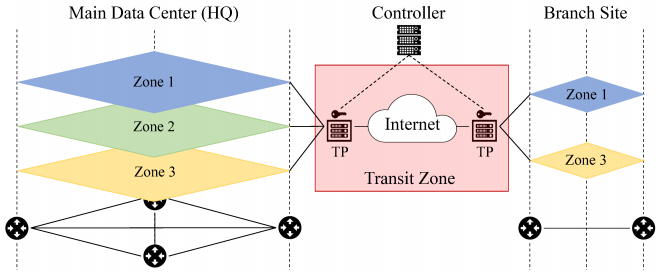
\includegraphics[width =0.48\textwidth]{img/mondrian_overview.png}
	\caption{MONDRIAN Overview\cite{kwonmondrian}}
	\label{MONDRIAN Overview}
\end{figure}

%\todo{\\
%    - What is MONDRIAN used for\\
%    - What does it replace\\
%    - What are zones/zone-transitions\\
%    - Show placement of TPs and MONDRIAN Controller
%}
\subsubsection{MONDRIAN Controller}
A MONDRIAN Controller is the brain of a MONDRIAN deployment. It hosts the databases containing all the information that is used by the \acsp{TP}, including the zone transition policies. Therefore, it needs to be reachable by the \acsp{TP} and is typically exposed to the Internet. Even though for redundancy reasons there might be multiple instances of a MONDRIAN Controller, all of them need to be synchronized. This means that logically there is just one MONDRIAN Controller. Furthermore, a MONDRIAN Controller exposes a \acs{REST}ful \acs{API} (\acl{API}), which allows an administrator to update the data which is stored on the MONDRIAN Controller. 

%\todo{\\
%    - Explain what a MONDRIAN Controller is used for\\
%    - Controller logically centralizes the management of zone transition policies
%}
\subsubsection{Translation Point}
A \acl{TP} has two main responsibilities. It needs to check the authorization of zone transitions according to the zone transition policies and it provides an \acs{IP}-tunneling functionality, comparable to a \acs{VPN}. The construction of a \acs{TP} is very modular. It consists of three modules. The \textbf{Core Module} is responsible for simple parsing and packet handling activities. The \textbf{Transition Module's} responsibility is zone transition authorization and the \textbf{Authentication Module} provides the tunneling mechanism.

%\todo{\\
%    - One TP per site\\
%    - transition authorization\\
%    - IP-tunneling
%}
\paragraph{Transition Module}
The Transition Module checks packets against policies of the form shown in formula \ref{policy}. Note that since we are using zone-IDs, the policies are independent of site or subnet specific information. If the 5-tuplet matches a packet, the $action$ takes effect. Possible actions are $forwarding$, $drop$ and $established$, which are comparable to actions found in \texttt{iptables}, but with a zone level granularity. The attribute $proto$ signifies the transport layer protocol. Currently \acs{TCP} (\acl{TCP}) and \acs{UDP} (\acl{UDP}) are supported. All of the fields in the 5-tuplet can also be wildcards, which means that the zone-ID, port or protocol can be arbitrary. 
\begin{equation}\label{policy}
    <zoneID_{dst}, port_{dst}, zoneID_{src}, port_{src}, proto>\Rightarrow <action>
\end{equation}
%\todo{Authorize zone transitions based on policies (5-tuplets,  action)}    

\paragraph{Authentication Module}
The Authentication Module is responsible for guaranteeing confidentiality, authenticity and end-host anonymity of packets, which traverse the untrusted Internet or \acs{WAN} (\acl{WAN}). It achieves that by encrypting the original \acs{IP} (\acl{IP})-packet and passing it together with an authentication token into a MONDRIAN-packet, which is basically an additional \acs{IP}-layer with an authentication token as metadata and the encrypted \acs{IP}-packet as payload. The authentication token consists of a type identifier, the destination's zone-ID, a timestamp, a nonce as well as a \acs{MAC} (\acl{MAC}). To perform the authentication as well as the encryption/decryption, MONDRIAN uses symmetric cryptography with keys that can be dynamically derived according to the \acs{DRKey} (\acl{DRKey}) \cite{perrig2017opt} derivation scheme. The derived keys provide authenticity on a site-to-zone level granularity, which means that the derived key depends on the site of the sender and on both the site as well as the zone of the destination.

%\todo{\\
%    - Create MONDRIAN packet\\
%    - IP-tunneling site-to-zone level\\
%    - protect confidentiality \& integrity of inter-domain traffic
%}

\subsection{Data Center Networking}\label{Data Center Networking}
Networking in data centers is different in many ways from networking in corporate networks or \acs{Telco} (\acl{Telco}) networks. Topologies are much more standardized and specialized, most of the infrastructure is virtualized and performance is essential.

%\todo{Highlight difference between networking in corporate networks (north-south vs east-west traffic)}
\subsubsection{Topology}
Network topologies in data centers are highly optimized for the kind of traffic they need to be able to handle and the desired properties or assurances the use case requires. These properties can range from minimal latency between hosts to bandwidth guarantees and congestion prevention. Mostly however, it boils down to saving costs while having the performance that is required by the application. While there exist many experimental topologies like Fat-tree \cite{LeisersonFatTree}, Jelly Fish \cite{singla2012jellyfish}, DCell \cite{guo2008dcell} or BCube \cite{guo2009bcube} to name a few, most of the topologies are a variation of the Leaf-Spine topology, where scalability is often achieved by using clos networks to replace switches with too few ports. Typically, data center topologies are built up using a three-tier layout consisting of a core layer, an aggregation layer and an access layer.
%\todo{\\
%    - Specialized for the traffic that it needs to handle\\
%    - hierarchical setup\\
%    - leave-spine, clos, etc.\\
%    - experimental topologies --> flexibility needed
%}
\subsubsection{Virtualization}
In data centers we have an extremely high degree of virtualization. End-hosts are usually \acsp{VM}, containers or entire Kubernetes clusters. However, not only end-hosts are virtualized. Many of the network functions like learning switches, routers, load balancers or even firewalls are virtualized into \acsp{VNF} (\aclp{VNF}). \acl{NFV} has traditionally been realized by simply deploying a \acs{VM}, which implements the desired functionality. With the gaining popularity of \acs{SDN}, more and more \acsp{VNF} (\aclp{VNF}) are implemented as an application running on top of an \acs{SDN} controller. Usually, the switch a host is directly connected to is the virtual switch, which is a part of the hypervisor and connects the VMs to each other and to the rest of the network. These virtual switches are often based on the \acs{OVS} (\acl{OVS}), which is a virtual switch that integrates well with OpenFlow, the de facto standard southbound \acs{SDN} protocol.

%\todo{\\
%    - Hosts = VMs, Containers\\
%    - network functions are often virtualized\\
%    - Hypervisors connect VMs via virtual switches to the rest of the network (mostly using OVS)
%}
\subsubsection{Performance}
In data centers, the computing resources are heavily monetized. A decrease in performance therefore results in immediate money loss. Many applications in data centers require the close collaboration between multiple hosts. Meaning that there's a lot of communication happening between hosts within the same data center. Consequently,  the performance bottleneck many applications experience lies in the network, which results in extremely high performance requirements for \acsp{VNF}, especially for \acsp{VNF} that affect east-west traffic, which makes up about 80\% of all network traffic in a typical data center \cite{talpurnetwork}. Data center networks are highly specialized for this kind of east-west traffic. Traffic engineers make sure that the strict performance requirements are met. It is therefore paramount that a new \acs{VNF} does not divert traffic from the originally intended route unless it's absolutely necessary.

%\todo{\\
%    - Performance is important\\
%    - bad performance = loss of money\\
%    - east-west performance is the most important 80\% \\ 
%    - DC networks are highly optimized for performance\\
%    - Don't divert traffic from original route
%}
\subsection{Software Defined Networking}
Networks based on \acs{SDN} are built up in three layers. The Infrastructure Layer consists of \acs{SDN} switches, which are controlled by an \acs{SDN} controller, which is located in the Control Layer. The topmost layer is the Application Layer, which is where business applications reside \cite{braun2014software}. The communication between the Infrastructure Layer and the Control Layer happens using a southbound protocol. The de facto standard for southbound \acs{SDN} protocols is called OpenFlow \cite{braun2014software}. While it's not the only southbound protocol, it is by far the most prominent one. As an interface between the Control Layer and the Application Layer, we have northbound interfaces. Since these interfaces are specific to the \acs{SDN} controller they are based on, there exists no standard for northbound interfaces. Some of the more popular \acs{SDN} controllers are Floodlight, HP VAN, POX, NOX or RYU \cite{tijare2016northbound}. Each of them has its own northbound \acs{API}. Some of the northbound interfaces are \acs{REST}ful \acsp{API}, which are usually used when a proactive strategy is employed, meaning that flow table entries are statically installed on the \acs{SDN} switches. If we employ a reactive strategy, meaning that we react to packets being sent to the \acs{SDN} controller via a packet-in message, then \acs{REST}ful \acsp{API} are not sufficient and we need a non-\acs{REST}ful \acs{API}. 
%\todo{\\
%    - Controller controlling switches\\
%    - Southbound protocol: OpenFlow = defacto standard\\
%    - Northbound API: No defacto standard \\
%    - Proactive vs. Reactive approach
%}
\subsection{Network Function Virtualization}
Virtualizing network functions has many benefits. It increases scalability, flexibility and resiliency. New networking components can be created and destroyed dynamically, without the need to move around physical hardware. This means that entirely new topologies can be created and reconfigured on the go, making it possible to meet different requirements at different points in time. Such a high degree of flexibility is needed in large data centers, where \acsp{VM} can be moved around and where traffic patterns can change instantly. While \acsp{VNF} are relatively new, there are already efforts to standardize \acs{NFV}. This process is mainly advanced by an organization called \acs{ETSI} (\acl{ETSI}).

Traditionally, \acsp{VNF} have been implemented on top of \acsp{VM}. This approach has the advantage that the \acsp{VNF} can perform any task that the underlying hardware is capable of handling. The major disadvantage is that \acsp{VM} can be quite resource consuming and take a relatively long time to spin up and down. Furthermore, \acsp{VM} require general purpose hardware, meaning that such \acsp{VNF} can't easily take advantage of specialized hardware like the one that can be found in switches. With the raising popularity and increasing maturity of \acs{SDN}, developers started implementing network functions as \acs{SDN} business applications. This has the advantage that some of the workload can be offloaded to the switches, where it's handled more efficiently and faster. However, not everything can be offloaded to \acs{SDN} switches. Computationally expensive operations like encryption and decryption can't be performed by switches. Since switches need to be very fast, they only support simple matching operations and can make forwarding decisions based on these matches.

%\todo{\\
%    - Standardization of NFV  \\
%    - Classical NFV based on VMs/Containers \\
%    - NFV based on SDN (Benefits, limitations)
%}

%\subsection{Related Work}
%The most important paper related to this thesis is of course the original MONDRIAN paper, proposing the original design of MONDRIAN \cite{kwonmondrian}. 
%
%What modern data centers look like and what concepts exist in the field of \ac{SDDC} is discussed in a whitepaper about VMware\texttrademark's NSX data center platform \cite{vmware2021nsx}. Current research questions concerning cloud data centers and where in data centers high costs occur and what the challenges are to minimize them is discussed in the paper \textit{The Cost of a Cloud: Research Problems in data center Networks} \cite{greenberg2008cost}.
%
%Regarding \ac{SDN}, there is a paper written by Intel\texttrademark,  discussing how a \ac{DPDK} enabled \ac{OVS} can enable \ac{SDN} and \ac{NFV} transformation \cite{intel2015OVS}. A great overview over the numerous northbound interfaces that exist for \ac{SDN} is provided by a paper called \textit{The Northbound APIs of Software Defined Networks} \cite{tijare2016northbound}. For gaining a basic understanding of the overall concepts of \ac{SDN}, I can recommend the book \textit{Software Defined Networks} by Paul Goransson and Chuck Black \cite{goransson2014SDN}.
%
%In the field of \ac{NFV} there exist a paper highlighting the benefits, enablers and challenges for \ac{NFV} \cite{att2012NFV}. This paper is a collaborative work of many major \ac{Telco} companies and has been presented at the \textit{\ac{SDN} and OpenFlow World Congress}.



%\todo{ \\
%	- original mondrian paper \cite{kwonmondrian}\\
%	- what DCs look like \cite{vmware2021nsx}\\
%	- what is important in DCs \cite{greenberg2008cost}\\
%	- OVS for SDN based NFV with DPDK \cite{intel2015OVS}\\
%	- Northbound APIs \cite{tijare2016northbound}\\
%	- Basics about SDN \cite{goransson2014SDN}\\
%	- NFV \cite{att2012NFV}
%}

\section{Overview}
\label{sec:overview}
% \chapter{Overview}
This chapter provides an overview over different aspects that we need to take into consideration when developing a new design for MONDRIAN. These aspects will explain why we came up with certain design principles.

\subsection{Goals}
For our new design to comply with the original specification of MONDRIAN, we need to make sure that the logically centralized nature of MONDRIAN is preserved. Furthermore, we should at least logically still have just one \acs{TP} per site. Regarding the cryptographic operations a \acs{TP} performs, we still require a site-to-zone level granularity for the symmetric keys. Considering the format of the policies, we still want a mapping between the 5-tuplet to one of the three actions as described in formula \ref{policy}. Any of the five properties can be specified as a wildcard and the protocols we consider in the policies are the transport layer protocols \acs{TCP} and \acs{UDP}. Finally, we want the entire mechanism to be easily integratable into the existing infrastructure we typically find in a modern data center.

%\todo{\\
%    - Logically Centralized property must be preserved\\
%    - Concept of one TP per site should stay the same \\
%    - Encryption/authentication on site-to-zone level\\
%    - Integrateable in DCs\\
%    - nature of policies should be preserved (support for wildcards, 3 actions + default, proto=transport layer)
%}
\subsection{Assumptions}
In order to justify the design decisions we're making, we have to define what we assume about the data centers in which we want to employ MONDRIAN. Firstly, we assume that the data centers use \acs{SDN} and in particular have OpenFlow switches already in place. Then we assume that the different \acs{SDN} components are placed with great care into the Service Function Chain (\acs{SFC}), meaning that if MONDRIAN decides to disallow a zone transition, no other service function will allow the zone transition. We also require that the \acs{SDN} installation follows best practices, such that we can rely on OpenFlow to work as expected, without any attacker being able to interfere with the protocol.% and that OpenFlow traffic is secured using \acs{TLS} (\acl{TLS}), which unfortunately is not mandatory in OpenFlow \cite{agborubere2017openflow}. \todo{rewrite and if TLS stuff is removed make sure TLS is written out somewhere}

Regarding robustness and resiliency, we assume that standard mechanisms are in place to ensure fast failover and disaster recovery. Standard backup procedures should be applied to backup MONDRIAN specific data just as any other security relevant data.

Finally, we assume that there is an existing \acs{PKI} (\acl{PKI}) in place, which ensures the security of all traffic that is using asymmetric cryptography. The root certificate will be present wherever it is needed.
%\todo{\\
%    - Networking happens using SDN (OpenFlow Switches)\\
%    - Placement of SDN components in the service function chain happens with great care\\
%    - Security of SDN communication is ensured using best practices \cite{agborubere2017openflow}\\
%    - PKI is in place\\
%    - Standard mechanisms for resiliency are in place 
%}
\subsection{Requirements}
As discussed in section \ref{Data Center Networking}, it is essential that new components in a data center don't divert traffic from the original route, as it is most likely the optimal route for this specific application. Especially east-west traffic cannot be subject to any delays or diversions. This means that zone transitions need to be authorized wherever routing is performed since zone transitions are always transitions into other subnets, which requires a routing functionality to be in place. In \acs{SDN} based data center networks, routing can happen at any \acs{SDN} switch.

Finally, the solution must be scalable and integrate well with already existing technologies, first and foremost with \acs{SDN}.

%\todo{ \\
%    - Traffic should not be diverted -- transitions checked where routing happens \\
%    - East-west performacne can not be compromised \\
%    - Solution must be scalable and integrate well with existing technologies 
%}
\subsection{Design Principles}
Due to the end-host anonymity MONDRIAN provides, it is necessary to decrypt inter-domain traffic at the gateway of a data center. As soon as a packet enters the data center's network fabric, it needs to be known who the end-hosts are, such that routing can be performed. For this to happen, we need to lift end-host anonymity and hence decrypt the MONDRIAN packet. However, if we placed the \acs{TP} at the gateway of a data center, then all of the east-west traffic would be heavily diverted and congestion would be unavoidable. In order to prevent traffic from being diverted, we need to implement the functionality of the Transition Module as close to the end-hosts as possible. Meaning, it should be implemented in the virtual switches of the hypervisors. 

Since the functionality of the Authentication Module and the functionality of the Transition Module can't be implemented at the same physical location, we need to virtualize the concept of a \acs{TP} and introduce a virtual component we call \acs{vTP} (\acl{vTP}). A \acs{vTP} consists of an \textbf{Endpoint \acs{TP}}, implementing the functionality of the Transition Module by incorporating an \acs{SDN} approach and a \textbf{Gateway \acs{TP}}, implementing the functionality of the Authentication Module by following a classical \acs{VM} / container-based \acs{NFV} approach. 

Figure \ref{vTP Overview} shows the schematic setup of a \acs{vTP}. Even though there is just one Gateway \acs{TP} and one Endpoint \acs{TP} present in the figure, there's nothing preventing us from having multiple instances of these components to improve scalability and robustness. Note that for the setup to be a proper MONDRIAN deployment, we also need a MONDRIAN controller, which is connected to both the Gateway \acs{TP} and the Endpoint \acs{TP}. The end-hosts will be connected to the switches which are managed by the \acs{SDN} controller hosting the Endpoint \acs{TP} as a business application. The Gateway \acs{TP} will on the one side be connected to the outside world, namely the Internet or some \acs{WAN}, whereas on the other side it will be connected to a gateway, which is responsible for setting up the routes for the inter-domain traffic. It's important to note that neither the Endpoint \acs{TP} nor the Gateway \acs{TP} are responsible for routing activities.

%\todo{continue here... explain connectivity with mondiran controller, endpoint tp = sdn app, gateway tp = VM}

\begin{figure}[t]
	\centering
	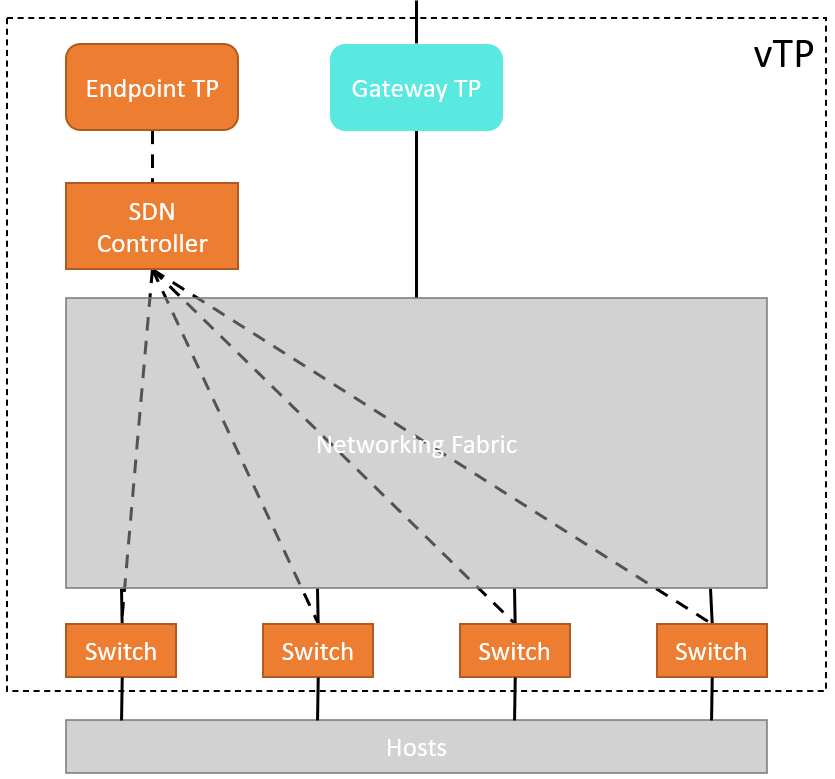
\includegraphics[width =0.48\textwidth]{img/vTP2.png}
	\caption{Conceptual overview of a \acl{vTP}}
	\label{vTP Overview}
\end{figure}

%\todo{ \\
%    - vTP keeps it logically centralized \\
%    - Splitting up the TP (explain why decryption needs to happen at the Gateway and why authorization needs to happen close to the Hosts) \\
%    - Discuss placement and connectivity of components [Fig]
%}

\section{Design}
\label{sec:design}
% \chapter{Design}
In this chapter, we discuss the design of the individual MONDRIAN components, as well as what design changes we come up with to make the MONDRIAN version more suitable for the data center environment. In particular, we have a look at the design of the MONDRIAN Controller, the Endpoint \acs{TP} and the Gateway \acs{TP}.


\subsection{MONDRIAN Controller}
Regarding the MONDRIAN Controller, we don't introduce any new concepts. Meaning that design wise it is identical to the MONDRIAN Controller from the original MONDRIAN design. This is useful since like this we can seamlessly combine traditional MONDRIAN deployments with the adapted version, which is designed specifically for data centers.

However, some details have not been fully specified in the original MONDRIAN design and are therefore worth pointing out. The current \acs{PoC} (\acl{PoC}) implementation of the current MONDRIAN Controller doesn't support the policies as described in the paper \cite{kwonmondrian} but instead just matches the source and destination zones. In our design however, we consider the full 5-tuplet as described in formula \ref{policy} and allow all fields to be wildcards. As protocols, we consider the transport layer protocols \acs{UDP} and \acs{TCP}. Furthermore, since we secure the control plane traffic between the MONDRIAN Controller and the Gateway \acs{TP} and the Endpoint \acs{TP} using asymmetric cryptography, we assume that we have a standard \acs{PKI} in place, which handles the distribution of the certificates. In our implementation we however just simulate the \acs{PKI} by previously distributing the certificates, just like it is done in the \acs{PoC} implementation of the original MONDRIAN.

%\todo{ \\
%    - Left as in the original design \\
%    - Implementation also considers wildcards and full 5-tuplet \\
%    - Communication secured with asymmetric crypto
%}
\subsection{Endpoint TP}
The Endpoint \acs{TP} is designed to be an application, which is running on top of an \acs{SDN} controller. It employs a reactive \acs{SDN} strategy, meaning that the first packet of a new flow will generate a packet-in message, which is sent to the \acs{SDN} controller. On the \acs{SDN} controller, there will be a processing pipeline, where packet-in handlers of different applications will process the packet-in message sequentially. Since an Endpoint \acs{TP} only allows or disallows traffic, it should be placed first in the \acs{SFC}. This means that the \acs{SDN} controller has to ensure that the Endpoint \acs{TP}'s packet-in handler is processed first. 

When a packet-in message is processed by an Endpoint TP, it first must parse the necessary header information such as the source and destination address, the source and destination port as well as the transport layer protocol. Then it will query the Transfer Module, where the packet is matched against the policies relevant for this site. Based on the outcome of this check, the Endpoint \acs{TP} then installs a flow table entry on the switch that generated the packet-in message. This means that following packets of this flow won't generate new packet-in messages for as long as the flow table entry didn't expire. To preserve the order of the \acs{SFC} on the \acs{SDN} switches, different \acs{SDN} applications are typically implemented in different flow tables. Since the Endpoint \acs{TP} is supposed to be the first service, it will install its flow table entries in flow table zero. The next service (e.g. a learning switch) will be implemented in flow table one. If an Endpoint \acs{TP} allows a flow, then the action will simply be a \texttt{GotoTable(1)} action, which allows the second service in the \acs{SFC} to process the packet. If the Endpoint \acs{TP} decides to drop a packet, then the OpenFlow action will be a \texttt{drop}, meaning that no subsequent service will be allowed to process the packet. 

It is worth pointing out that such a design has the benefit that only a fraction of all packets need to be processed by the Endpoint \acs{TP} application while most packets are forwarded or dropped very efficiently by the \acs{SDN} switches. This offers the Endpoint \acs{TP} the scalability and performance that is needed in modern data centers.
%todo{ \\
%   - App based on SDN Controller \\
%   - Explain Service Function Chaining using flow tables and chaining packet-in handlers \\
%   - Explain why reactive approach was chosen \\
%   - Explain what parts are handled by the switch and what by the Endpoint TP app 
%
\subsection{Gateway TP}
At the Gateway \acs{TP} the conversion between \acs{IP} and MONDRIAN packets takes place. Since the payload of a MONDRIAN packet is the encrypted original \acs{IP} packet, the Gateway \acs{TP} needs to be powerful enough to perform line-rate encryption and decryption. Such costly operations can't be handled by a simple \acs{SDN} switch but instead require more powerful hardware, ideally supporting hardware accelerated cryptographic operations such as the \acs{AES-NI} (\acl{AES-NI}) instruction \cite{rott2012AESNI}.

We therefore design the Gateway \acs{TP} as a traditional middlebox. However, we still need to ensure that it integrates into the highly virtualized environment that we find in a data center. Therefore, we design the Gateway \acs{TP} to be a \acs{VM}/container-based \acs{VNF}. \aclp{VM} can perform line-rate cryptographic operations, as we can see when we consider virtualized \acs{VPN} servers.

Deploying a Gateway \acs{TP} in a \acs{VM} or in a container allows us to quickly spin up/down new instances of a Gateway \acsp{TP} as the demand increases or decreases. Especially containers can be started and stopped within seconds. 

Another advantage of the new design is that the Gateway \acs{TP} is no longer in charge of authorizing zone transitions, meaning that it can be kept leaner and can therefore be implemented more efficiently than the original \acsp{TP}. At the same time it only has to deal with inter-domain traffic (see figure \ref{DC MONDRIAN Overview}), meaning that a Gateway \acs{TP} will be able to handle more hosts than a traditional \acs{TP}. 

\begin{figure}[t]
	\centering
	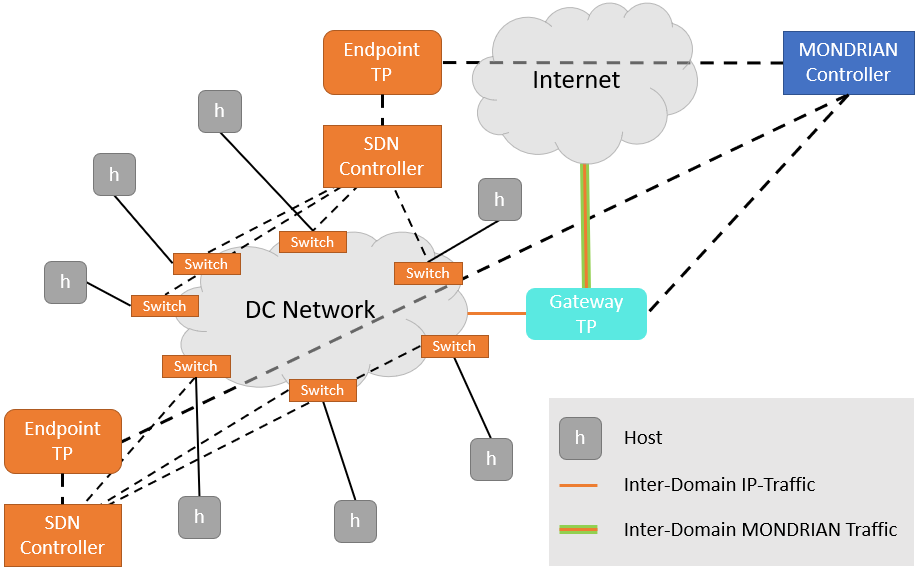
\includegraphics[width =0.48\textwidth]{img/DC_Mondrian_overview2.png}
	\caption{\acs{DC} (\acl{DC}) MONDRIAN Overview}
	\label{DC MONDRIAN Overview}
\end{figure}

%\todo{ \\
%    - Encryption/Decryption requires more advanced hardware than Switches \\
%    - Virtual middlebox can provide line-rate crypto \\
%    - Deploying it as VMs makes scalability easy -- spin up more if needed \\
%    - High performance implies that only the essential tasks should performed there (move authorization into the Endpoint TPs)
%}

\section{Implementation}
\label{sec:implementation}
% \chapter{Implementation}
This chapter provides detailed information about the implementation of the individual MONDRIAN components, as well as their modules.

\subsection{MONDRIAN Controller}
The MONDRIAN Controller is implemented in Go and is fairly similar to the MONDRIAN Controller of the original MONDRIAN design. The backend database is an SQLite database, with a structure defined in listing \ref{MONDRIAN Controller Database}. The connection to the controller is secured by using \acs{TLS} (\acl{TLS}). The certificates are previously distributed in our setup while in a production environment they would be obtained via a standard \acs{PKI}.

Since the MONDRIAN Controller is implemented in Go, the code is structured into different packages, which we individually discuss below.

\paragraph{main} This package is the entry-point of the MONDRIAN Controller. It binds the routes to the endpoints, which are documented in table \ref{MONDRIAN Controller API}. It then listens and serves on the predefined port.
\paragraph{handler} The handler package contains the implementation of the different handlers, which handle the \acs{HTTP} (\acl{HTTP}) requests coming from a client (Admin, Gateway \acs{TP} or Endpoint \acs{TP}).
\paragraph{db} This package is used to set up the database according to the schema shown in listing \ref{MONDRIAN Controller Database}. Furthermore, it provides the implementation of functions that interact with the database. Most queries and statements are quite straight forward. The two queries, which are a bit more complicated are at the same time also the most important ones, since they fetch site specific data from the database. The queries for getting the relevant subnets and zone transition policies are shown in listings \ref{Get Subnets Query} and \ref{Get Transitions Query} respectively.
\paragraph{types} This package contains the type definitions for zones, sites, subnets and zone transition policies.
\paragraph{api} The \texttt{api} package provides a Go \acs{API} for interacting with the database of the MONDRIAN Controller. This \acs{API} can be used by an administration frontend.

%\begin{table*}[h]\centering
%    \ra{1.3}
%    \begin{tabular}{@{}p{.2\textwidth}p{.8\textwidth}@{}}\toprule
%    \textbf{Package} & \textbf{Description} \\\midrule
%    main & This package is the entry-point of the MONDRIAN Controller. It binds the routes to the endpoints, which are documented in table \ref{MONDRIAN Controller API}. It then listens and serves on the predefined port.\\
%    handler & The handler package contains the implementation of the different handlers, which handle the \ac{HTTP} requests coming from a client (Admin, Gateway \ac{TP} or Endpoint \ac{TP}).\\
%    db & This package is used to set up the database according to the schema shown in listing \ref{MONDRIAN Controller Database}. Furthermore, it provides the implementation of functions that interact with the database. Most queries and statements are quite straight forward. The two queries, which are a bit more complicated are at the same time also the most important ones since they fetch site specific data from the database. The queries for getting the relevant subnets and zone transition policies are shown in listings \ref{Get Subnets Query} and \ref{Get Transitions Query} respectively.\\
%    types & This package contains the type definitions for zones, sites, subnets and transition policies.\\
%    api & The \texttt{api} package provides a Go \ac{API} for interacting with the database of the MONDRIAN Controller. This \ac{API} can be used by an administration frontend.\\
%    \bottomrule
%    \end{tabular}
%    \caption{Package Documentation}
%    \label{Package Documentation}
%    \end{table*}

%\todo{ \\
%    - Implemented in Go \\
%    - Using SQLite \\
%    - API definition 
%}
%\newpage
%\definecolor{codegreen}{rgb}{0,0.6,0}
%\definecolor{codegray}{rgb}{0.5,0.5,0.5}
%\definecolor{codepurple}{rgb}{0.58,0,0.82}
%\definecolor{backcolour}{rgb}{0.95,0.95,0.92}
%
%\lstdefinestyle{mystyle}{
%    backgroundcolor=\color{backcolour},   
%    commentstyle=\color{codegreen},
%    keywordstyle=\color{magenta},
%    numberstyle=\tiny\color{codegray},
%    stringstyle=\color{codepurple},
%    basicstyle=\ttfamily\footnotesize,
%    breakatwhitespace=false,         
%    breaklines=true,                 
%    captionpos=b,                    
%    keepspaces=true,                 
%    numbers=left,                    
%    numbersep=5pt,                  
%    showspaces=false,                
%    showstringspaces=false,
%    showtabs=false,                  
%    tabsize=2,
%	morekeywords = {DISTINCT, WITH, REFERENCES, TEXT, AUTOINCREMENT},
%	otherkeywords = {IS}
%}
%
%\lstset{style=mystyle}

\begin{lstlisting}[language=SQL, breaklines=True, caption=Get Subnets Query, label=Get Subnets Query, sensitive=true]
WITH tp_zones
	AS (SELECT DISTINCT zone 
		FROM   subnets 
		WHERE  tp_address = ?), 
possible_dests 
	AS (SELECT DISTINCT dest
		FROM   transitions 
		WHERE  (src IN tp_zones OR src = 0 OR src IS NULL) AND dest NOT IN tp_zones), 
possible_src 
	AS (SELECT DISTINCT src
		FROM  transitions 
		WHERE  (dest IN tp_zones OR dest = 0 OR dest IS NULL) AND src NOT IN tp_zones),
dest_wildcard
	AS (SELECT DISTINCT src
		FROM transitions 
		WHERE dest IS NULL OR dest = 0),
src_wildcard
	AS (SELECT DISTINCT dest
		FROM transitions
		WHERE src IS NULL OR src = 0), 
wildcard_zone_count_src
	AS(	SELECT DISTINCT count(dest) 
		FROM src_wildcard
		WHERE dest IN tp_zones),
wildcard_zone_count_dest
	AS(	SELECT DISTINCT count(src) 
		FROM dest_wildcard
		WHERE src IN tp_zones)
SELECT net_ip, net_mask, zone, tp_address 
	FROM   subnets 
	WHERE  zone IN tp_zones OR zone IN possible_dests
	   OR zone IN possible_src
	   OR ((SELECT count(*) FROM tp_zones JOIN dest_wildcard WHERE zone = src) > 0)
	   OR ((SELECT count(*) FROM tp_zones JOIN src_wildcard WHERE zone = dest) > 0)
\end{lstlisting}
%finecolor{codegreen}{rgb}{0,0.6,0}
%finecolor{codegray}{rgb}{0.5,0.5,0.5}
%finecolor{codepurple}{rgb}{0.58,0,0.82}
%finecolor{backcolour}{rgb}{0.95,0.95,0.92}
%
%tdefinestyle{mystyle}{
% backgroundcolor=\color{backcolour},   
% commentstyle=\color{codegreen},
% keywordstyle=\color{magenta},
% numberstyle=\tiny\color{codegray},
% stringstyle=\color{codepurple},
% basicstyle=\ttfamily\footnotesize,
% breakatwhitespace=false,         
% breaklines=true,                 
% captionpos=b,                    
% keepspaces=true,                 
% numbers=left,                    
% numbersep=5pt,                  
% showspaces=false,                
% showstringspaces=false,
% showtabs=false,                  
% tabsize=2,
%morekeywords = {DISTINCT, WITH, REFERENCES, TEXT, AUTOINCREMENT},
%otherkeywords = {IS}
%
%
%tset{style=mystyle}

\begin{lstlisting}[language=sql, breaklines=True, caption=Get Transitions Query, label=Get Transitions Query, sensitive=true]
WITH relevant_zones 
	AS (SELECT DISTINCT zone 
		FROM   subnets 
		WHERE  tp_address = ?) 
SELECT policyID, src, dest, srcPort, destPort, proto, action
	FROM   transitions 
	WHERE  src IN relevant_zones 
	   OR dest IN relevant_zones
	   OR src IS NULL
	   OR dest IS NULL
\end{lstlisting}

% \onecolumn
\begin{table}[t]
\begin{tabular}{@{}p{.15\textwidth}p{.67\textwidth}@{}}\toprule
\textbf{Route} & \textbf{Endpoint} \\\midrule
\multicolumn{2}{c}{\textit{Used by Endpoint TP and Gateway TP}}\\\midrule
/api/get-subnets & Returns the subnets which are located at the site specified in the body of the request or the subnets which are reachable from this site according to the policy database.\\
\bottomrule
\multicolumn{2}{c}{\textit{Used by Endpoint TP}}\\\midrule
/api/get-transitions & Returns the policies which are relevant for the hosts of the site specified in the body of the request.\\
\bottomrule
\multicolumn{2}{c}{\textit{Used for Testing}}\\\midrule
/ & This endpoint is just used to test the reachability of the MONDRIAN Controller.\\% It simply answers with \texttt{Hello from the Controller}.\\ 
\bottomrule
\multicolumn{2}{c}{\textit{Used by Administrator}}\\\midrule
/api/get-all-sites & Returns all sites stored in the database of the MONDRIAN Controller.\\
/api/get-all-zones & Returns all zones stored in the database of the MONDRIAN Controller.\\
/api/get-all-subnets & Returns all subnets stored in the database of the MONDRIAN Controller.\\
/api/get-all-transitions & Returns all zone transition policies stored in the database of the MONDRIAN Controller.\\
/api/insert-sites & Inserts a list of sites into the database.\\
/api/insert-zones & Inserts a list of zones into the database.\\
/api/insert-subnets & Inserts a list of subnets into the database.\\
/api/insert-transitions & Inserts a list of policies into the database.\\
/api/delete-sites & Delete all sites which are listed in the list of sites in the body of the request.\\
/api/delete-zones & Delete all zones which are listed in the list of zones in the body of the request.\\
/api/delete-subnets & Delete all subnets which are listed in the list of subnets in the body of the request.\\
/api/delete-transitions & Delete all transitions which are listed in the list of transitions in the body of the request.\\
\bottomrule
\end{tabular}
\caption{MONDRIAN Controller API}
\label{MONDRIAN Controller API}
\end{table}
% \twocolumn
    
\FloatBarrier
\subsection{Endpoint TP}
The Endpoint \acs{TP} is implemented as a RYU application which is based on the RYU \acs{SDN} controller \cite{RYU2021docs}. The RYU controller is based on Python and therefore provides a Python \acs{API} as a northbound interface. As a southbound protocol, the RYU controller uses the well-established OpenFlow protocol and supports its versions 1.0-1.5. Since OpenFlow version 1.3 seems to be the most established one, we choose version 1.3 for the implementation of the Endpoint \acs{TP}. However, it should be easy to upgrade it to version 1.4 or 1.5 since the code is mostly OpenFlow independent. The only hard requirement we have regarding the OpenFlow version is that we need to be able to match all fields that we find in the 5-tuplet of a MONDRIAN policy.

The support for a wide range of OpenFlow versions and the well maintained documentation of the Python \acs{API} together with the circumstance that Python is an ideal language for fast prototyping, led us to the decisions to use the RYU \acs{SDN} controller as a basis for the implementation of the Endpoint \acs{TP}.

The RYU \acs{SDN} controller ships with a so called \texttt{ryu-manager}, which is used to configure and start the \acs{SDN} controller and load and start the individual applications, which are implemented as Python classes, inheriting from the \texttt{app\_manager.RyuApp} class.

There are certain parameters, which have been set to a default in the \acs{PoC} implementation of the Endpoint \acs{TP} but would need to be fine-tuned to the needs of the environment in which the Endpoint \acs{TP} would be running. The fetcher, which fetches data from the MONDRIAN Controller has a \texttt{refresh\_interval} parameter, which is set to 30 seconds by default. Meaning that every 30 seconds it fetches new data from the MONDRIAN Controller. Increasing this interval means that the Endpoint TP is less responsive to policy changes but also has a lower overhead due to the fetching activities. Furthermore, flow table entries in OpenFlow can expire after some time depending on two types of timeouts that one can set. An \texttt{IDLE\_TIMEOUT} means that a flow table entry is removed if it didn't match a flow for the given amount of time. A \texttt{HARD\_TIMEOUT} on the other hand will forcibly cause the removal of a flow table entry that expired due to it, regardless of how often it matched a flow. Both timeouts can be set to infinity by setting their values to zero, which is what we do for table miss entries.

Subsequently, we discuss the role individual Python files of the code base of the Endpoint \acs{TP} play.

\paragraph{main.py} The main file is the starting point of an Endpoint \acs{TP}. It contains the \texttt{EndpointTP} class, which implements the \texttt{RyuApp}. The \texttt{EndpointTP} class contains the two main event handlers that we make use of. The function \texttt{switch\_features\_handler(self, ev)} is invoked whenever a switch gets newly connected to the RYU \acs{SDN} controller. In this function, we create an empty match, which means that it matches against every flow. Then we add a new flow table entry with this empty match, which has priority zero, meaning the lowest possible priority. Both the \texttt{HARD\_TIMEOUT} as well as the \texttt{IDLE\_TIMEOUT} are set to zero, such that the flow will never time out. This flow table entry is called a table miss entry and it takes effect whenever there's no other flow table entry that matched a specific flow. The action associated to this flow table entry is an \texttt{OFPP\_CONTROLLER} action, meaning that the packet will be sent to the \acs{SDN} controller and therefore to the Endpoint \acs{TP} via a packet-in message.

The second event handler is the \texttt{packet\_in\_handler(self, ev)} function. As the name suggests, it handles packet-in messages. It parses the necessary header information from the packet, queries the transfer module and installs a flow table entry either allowing or disallowing the flow based on the decision the transfer module made. Note that non-\acs{IP}v4 traffic will simply be ignored by the Endpoint \acs{TP}, meaning that it's the responsibility of other components to handle that kind of traffic.

\paragraph{start\_custom\_EndpointTP.py} An Endpoint \acs{TP} reads at startup some parameters from a \texttt{config.json} file. The script \texttt{start\_custom\_EndpointTP.py} allows us to update the content of this file by passing command line arguments to the script. It then starts the Endpoint \acs{TP} with the updated \texttt{config.json} file as well as other RYU services. Currently it starts a L2 switch, which is placed after the Endpoint \acs{TP} in the \acs{SFC}. This script is useful for the automated startup of different instances of an Endpoint \acs{TP}.

\paragraph{conn\_state.py} If a policy matches a flow where the action in the policy is \texttt{established}, the Endpoint \acs{TP} needs to keep a state such that it knows that it needs to allow the response traffic once it arrives at the Endpoint \acs{TP}. This state is needed to make sure that no response is allowed for which there wasn't an initiator of the connection. The class \texttt{ConnectionState} is basically a data structure where a connection can be added when initiated and looked up and removed once the responder sends its response. There's a mechanism in place that prevents the state from growing arbitrarily. If it exceeds a maximum number of entries (100 by default) then it simply removes the oldest connection from the state. Note that this is simply a protection mechanism and that the size is expected to be constant since for most initiations there will be a response.

\paragraph{const.py} The \texttt{Const} class is used to store some values that are constant during the execution of an instance of an Endpoint \acs{TP}. At startup, the class method \texttt{init\_const(self)} is invoked, which reads the parameters stored in the \texttt{config.json} file and makes them available to the Endpoint \acs{TP}.

\paragraph{fetcher.py} The \texttt{Fetcher} class stores a list of subnets and a list of zone transition policies. These two lists get regularly refreshed by a daemon thread, which fetches fresh data from the MONDRIAN Controller. The \texttt{refresh\_interval} is by default set to 30 seconds. 

The functions \texttt{get\_subnets()} and \texttt{get\_policies()} can be used to retrieve the current data from the fetcher. 

\paragraph{stats.py} The \texttt{Stats} class is used for the evaluation of the Endpoint \acs{TP}. When initializing a \texttt{Stats} object, the parameter \texttt{delta\_t} is set (by default it's 60 seconds), which is the time interval in which the number of occurrences of an event is recorded. To record an event we can simply invoke the \texttt{tick()} function of the \texttt{Stats} class. Every \texttt{delta\_t} seconds, the number of events recorded in the last interval will be written to a file.

\paragraph{sync.py} Different RYU applications might need some form of communication or synchronization amongst each other. For this purpose, we can set a context dictionary which can be used to create shared objects. The \texttt{Synchronizer} class is the class which will generate the shared object, which we need to ensure that the order of the \acs{SFC} is preserved. The decision of the Endpoint \acs{TP}, whether or not to allow a flow, is recorded in the \texttt{Synchronizer} object. Following RYU applications like the L2 switch can then still learn the mac addresses but before any of the following services decides to send a packet-out message, it needs to check with the \texttt{Synchronizer} to figure out if the traffic is allowed or not.

\paragraph{transfer\_module.py} The \texttt{TransferModule} is responsible for the policy checking. The function \texttt{check\_packet(self, packet)} takes in a packet object, finds the source and destination zone and checks the packet against the policies. If multiple policies match, then the one with the highest priority is chosen. The overall priority is determined by summing up partial priorities of individual fields whenever they are specified, meaning they are not wildcards. The different priorities of the individual fields of the 5-tuplet can be seen in table \ref{Policy Field Priorities}. The idea behind this weighting is that specified zones are always preferred over specified ports or protocol. Since destination ports are often bound to a service, while source ports can normally be chosen arbitrarily, we decided to weight a specified destination port equally with a specified pair of source port and transport layer protocol. If multiple policies with the same priority match, we break ties by simply choosing the policy with the higher policy-ID, since this will most likely be the newest policy.

The \texttt{check\_packet(self, packet)} function classifies a packet into one of six subsequently described categories.
\subparagraph{\texttt{FORWARDING}} The policy with the highest priority that matched the packet has \textit{"forwarding"} as an action.
\subparagraph{\texttt{DROP}} The policy with the highest priority that matched the packet has \textit{"drop"} as an action.
\subparagraph{\texttt{ESTABLISHED}} The policy with the highest priority that matched the packet has \textit{"established"} as an action.    
\subparagraph{\texttt{ESTABLISHED\_RESPONSE}} The packet could be the response to an established connection. Note that this classification is returned next to one of the other five classifications, which would be determining the action in case of the connection not being in the state and therefore not being established.
\subparagraph{\texttt{INTRA\_ZONE}} The source and the destination zone are the same. Intra-zone traffic will be allowed and the flow table entry will be more permissive since we don't have to match the ports nor the protocol.
\subparagraph{\texttt{DEFAULT}} The packet didn't match any policy and therefore a default action will be applied. In our case we simply drop that kind of traffic.

\begin{table}[t]
\centering
\begin{tabular}{@{}p{.15\textwidth}p{.1\textwidth}@{}}\toprule
    \textbf{Policy Field} & \textbf{Priority} \\\midrule
    Source Zone & +5\\
    Destination Zone & +5\\
    Source Port & +1\\
    Destination Port & +2\\
    Protocol & +1\\
    \bottomrule
\end{tabular}
    \caption{Policy Field Priorities}
    \label{Policy Field Priorities}
\end{table}


\paragraph{types.py} This file contains the type definitions for the MONDRIAN specific types like \texttt{Policy}, \texttt{Subnet} and \texttt{Zone} as well as the type definition for the \texttt{Packet} object, which is passed into the \texttt{check\_packet(self, packet)} function of the transition module.


%\todo{ \\
%    - RYU Controller with Python API \\
%    - Fetcher fetching data from MONDRIAN controller periodically\\
%    - Transition Module checking packet against policies \\
%    - Synchronizer = shared state between SDN Apps which is used to ensure that drop decissions are respected also by other handlers \\
%    - Conn state is used to allow established connections (argue why the state is no problem) \\
%    - Discuss Idle/Hard timeout
%}
% \newpage
\subsection{Gateway TP}
The Gateway \acs{TP} is implemented in Go, such that some concepts can be borrowed from the implementation of the \acs{TP} from the original MONDRIAN design. However, the original MONDRIAN implementation was based on top of the \acs{SCION} (\acl{SCION}) \cite{perrig2017scion} internet architecture, where as a Gateway \acs{TP} is implemented to work over an \acs{IP} based network. 

The standard way of manipulating \acs{IP} packets in Go is by using \texttt{gopackets} \cite{google2020gopacket}. For reading traffic from an interface, we use the \texttt{pcap} package, which is part of the \texttt{github.com/google/gopacket} module. 

The Gateway \acs{TP} basically is a forwarder, which reads packets from one interface, transforms them from MONDRIAN packets to \acs{IP} packets or vice versa and then sends the resulting packet out the other interface. This means that the Gateway \acs{TP} simply sits on the wire and performs the transformation but doesn't take responsibility for any other tasks like routing. The transformation to and from MONDRIAN requires a cryptographic operation, which in turn requires a symmetric key. This key is derived according to the \acs{DRKey} derivation scheme. This process requires communication between different Gateway \acsp{TP}. This communication happens via a separate interface and so does the communication with the MONDRIAN Controller. Like this control plane traffic and data plane traffic are completely separated.

Subsequently, we describe the functionality of the different packages of the Gateway \acs{TP}


\paragraph{main} The \texttt{main} package is the entry point of the Gateway \acs{TP}. It initializes the \texttt{config} package as well as the \texttt{logger} package. Then it creates a \texttt{forwarder} and starts it. After that it just waits while the \texttt{forwarder} is handling the traffic.

\paragraph{config} The \texttt{config} package contains some constants and also an initializer, which reads some parameters from the \texttt{config.json} file and makes these parameters available to the rest of the Gateway \acs{TP}.

\paragraph{types} This package contains the type definitions of the MONDRIAN types. Namely of \texttt{Site}, \texttt{Zone}, \texttt{Subnet} and \texttt{Transition}. It also contains the implementation of some helper functions, related to the handling of these types.

\paragraph{fetcher} The \texttt{fetcher} package implements a similar functionality as the fetcher of the Endpoint \acs{TP}. It starts a goroutine which regularly fetches data from the MONDRIAN Controller. It then provides the interfaces for other modules to read the zone and site information based a provided \acs{IP} address in a thread safe way.

\paragraph{keyman} The key manager has three main responsibilities. Firstly, it acts as a key server, providing an \acs{API} with which other Gateway \acsp{TP} can fetch the right L1 key. The \acs{API} is described in table \ref{Key Server API}. It also fetches L1 keys from remote \acsp{TP} if needed. Secondly, it internally performs the key derivations according to the \acs{DRKey} derivation scheme and also makes sure that the keys are always fresh. Thirdly, it provides an interface for other modules to get the right L2 key for a given source \acs{TP}, destination \acs{TP} and destination zone.

% \FloatBarrier
% \onecolumn
\begin{table}[t]
\centering
\begin{tabular}{@{}p{.08\textwidth}p{.38\textwidth}@{}}\toprule
    \textbf{Route} & \textbf{Endpoint} \\\midrule
    \multicolumn{2}{c}{\textit{Used for Testing}}\\\midrule
    / & This endpoint is just used to test the reachability of the Key Server. It simply answers with \texttt{Hello from the Key Server}.\\ 
    \bottomrule
    \multicolumn{2}{c}{\textit{Used by Gateway \acsp{TP}}}\\\midrule
    /api/Get-L1-Key & This endpoint is used to let a remote Gateway \acs{TP} fetch the L1-key from the local key server. If the local key server is $B$ and the request comes from $A$ then $B$ sends to $A$ the following key: $K_{A \to B}$\\ 
    \bottomrule
\end{tabular}
    \caption{Key Server \acs{API}}
    \label{Key Server API}
\end{table}
% \twocolumn

\paragraph{forwarder} The \texttt{forwarder} package starts a \texttt{fetcher} and a \texttt{keyman}. It then creates an interface handle by using \texttt{pcap} for both an internal as well as an external interface. The internal interface faces the data center's network and the external interface is exposed to the internet. The \texttt{forwarder} then reads from both interfaces, transforms the packets from \acs{IP} to MONDRIAN or from MONDRIAN to \acs{IP} and then sends the resulting packet out via the other interface respectively.

\paragraph{mondrian} This package contains the type definition of the MONDRIAN layer, which is used to create and parse gopackets. Since gopackets are designed to be a stack of protocol layers, which are then serialized into a buffer, we simply need to define a new layer if we want to create a new protocol such as MONDRIAN. A MONDRIAN packet is basically a layer stack consisting of an ethernet layer, an \acs{IP} layer and a MONDRIAN layer.

\paragraph{crypto} This package provides some functions for performing cryptographic operations. It uses open-source cryptographic libraries and creates an \acs{AEAD} (\acl{AEAD}) cipher, meaning that encryption and authentication can happen with only one operation. The cipher we use is an \acs{AES} (\acl{AES}) cipher in \acs{GCM} (\acl{GCM}) mode, which has the advantage that we can make use of the hardware accelerated \acs{AES-NI} instruction.

\paragraph{api} This package is the client \acs{API} provided by the MONDRIAN Controller. It is used by the \texttt{fetcher} to fetch data from the MONDRIAN Controller.

\paragraph{logger} The \texttt{logger} package is used to write some log information into a file. However, it should only be used if important and rarely occurring events take place, because writing to a file can severely impact the forwarding performance of the Gateway \acs{TP}.



%\todo{ \\
%    - Implemented in Go \\
%    - Using gopackets/pcap \\
%    - forwarder reading from interface, transforming, sending on other interface \\
%    - Keymanager using DRKey to establish shared secrets between sites \\
%    - fetcher periodically fetching data from MONDRIAN Controller
%}

\section{Evaluation}
\label{sec:evaluation}
% \chapter{Evaluation}
In this chapter, we show how we rigorously evaluate the functionality, performance and security of each MONDRIAN component individually, as well as together in a full MONDRIAN deployment. We present the findings and prove the practicality of the new design and the resulting implementation. 

\subsection{Functionality Evaluation}
\subsubsection{Mininet / Containernet}
In order to test out \acsp{VNF} and in particular \acs{SDN} applications, we need a way to emulate a network consisting of hosts, \acs{SDN} switches and \acs{SDN} controllers. The open-source network emulation software called \texttt{mininet} \cite{mininet2021webpage} provides a fast and efficient way of creating complex network topologies on a single physical or virtual machine. \texttt{mininet} separates hosts and switches by using lightweight \acs{OS} (\acl{OS}) virtualization. This means that hosts and switches have their own networking stack but share the file system, meaning that \texttt{mininet} is sufficient for testing out \acs{SDN} applications but is not ideal for testing out \acs{VM}/container based \acsp{VNF}. To provide isolation of the file system for virtual middleboxes like the Gateway \acsp{TP}, we use a network emulation framework called \texttt{containernet} \cite{peuster2018containernet}, which is based on \texttt{mininet} but additionally offers integration of containers as hosts in the network. 

Both \texttt{mininet} and \texttt{containernet} are based on Python and offer a rich Python \acs{API} to programmatically spin topologies up and down. For testbeds, which only employ the \acs{SDN} based Endpoint \acs{TP}, \texttt{mininet} is sufficient. However, as soon as we also use Gateway \acsp{TP}, we need the testbed to be based on \texttt{containernet}.


%\todo{\\
%    - What is it and how does it work (what is it used for) \\
%    - Why is Mininet not enough and why do we need containernet
%}
\subsubsection{Testbeds}
To test the functionality of the Endpoint \acs{TP}, the Gateway \acs{TP} as well as their combination in a full MONDRIAN deployment, we created three different testbeds. For all testbeds we use the same set of zone transition policies shown in figure \ref{Policy Database} but of course different configurations for the \textit{Sites}, \textit{Zone} and \textit{Subnet} tables as shown in figure \ref{fig:Testbed Configuration}.
\paragraph{EndpointTP\_testbed.py} The Endpoint \acs{TP} testbed is designed to test out the zone transition authorization mechanism the Endpoint \acs{TP} provides. It consists of two sites, three zones and five hosts in total. Each site has a special host (\texttt{h1}, \texttt{h2}) at the gateway of the site, which acts as a default gateway and performs routing between the sites. An overview of the testbed's layout is shown in figure \ref{Endpoint TP Testbed}. To prove the correct functionality of the Endpoint \acs{TP}, we need to consider four types of traffic and be able to generate them by initiating communication between two hosts. Which pairs of hosts we can use to generate the desired type of traffic is shown in table \ref{Types of Traffic}.

% \onecolumn
\begin{table}[t]
\centering
\begin{tabular}{@{}p{.18\textwidth}p{.27\textwidth}@{}}\toprule
    \textbf{Type of Traffic} & \textbf{Hosts to generate Traffic} \\\midrule
    Intra-Zone, Intra-Domain & $\{h11\}\leftrightarrow \{h12\}$\\ 
    Intra-Zone, Inter-Domain & $\{h11, h12\}\leftrightarrow \{h21\}$\\
    Inter-Zone, Intra-Domain & $\{h11, h12\}\leftrightarrow \{h13\}$\\
    Inter-Zone, Inter-Domain & $\{h11, h12, h13\}\leftrightarrow \{h22\}$ or $\{h13\}\leftrightarrow \{h21\}$\\
    \bottomrule
\end{tabular}
    \caption{Traffic Classification of Inter-Host Communication}
    \label{Types of Traffic}
\end{table}
% \twocolumn


\paragraph{GatewayTP\_testbed.py} The Gateway \acs{TP} testbed consists of two sites, each of them holding one end-host as well as one gateway router. Between the gateway router and the link simulating an internet connection, we have a Gateway \acs{TP}. Note that the gateway router is still needed since we don't want the Gateway \acs{TP} to be in charge for making routing decisions. The layout of the Gateway \acs{TP} testbed is shown in figure \ref{Gateway TP Testbed}. The additional switch that connects the Gateway \acsp{TP} is used for communication amongst Gateway \acsp{TP} for the sake of performing key establishment. Note that all control plane traffic (dashed lines) is completely separated from data plane traffic (solid lines). 

The correct behavior of the Gateway \acsp{TP} can be shown by either logging the packets each Gateway \acs{TP} receives or by using a traffic inspection tool such as wireshark \cite{wireshark2021}. 

\paragraph{MONDRIAN\_testbed.py} To test out a full MONDRIAN deployment, we created a MONDRIAN testbed (see figure \ref{MONDRIAN Testbed}). It consists of three sites, each hosting 3 hosts. In this testbed we have all three components of the new MONDRIAN design present and can prove that the Endpoint \acsp{TP}, the Gateway \acsp{TP} and the MONDRIAN Controller harmonize perfectly.

%\todo{\\
%    - Endpoint TP testbed \\
%    - Gateway TP testbed \\
%    - MONDRIAN testbed \\
%}



\subsubsection{Test Cases}
To rigorously test out certain properties of a testbed, we need a way to programmatically generate traffic between two hosts. For this purpose, we have the \texttt{TestUtil} class. It provides a set of functions that can be used for generating \acs{UDP}, \acs{TCP} or \acs{ICMP} (\acl{ICMP}) traffic between any two hosts. For testing \acs{ICMP} traffic, we simply let one host ping the other one and check how many packets get received. If the amount of received packages is bigger than zero, we consider the test as being successful. For generating \acs{UDP} or \acs{TCP} traffic we use \texttt{netcat} to create a server listening on a port and a client sending data via a specific port. This allows us to test policies which have the source and destination port specified. Since both hosts share the file system with \texttt{localhost}, we can simply dump the received data into a file and check if the sent data has been received successfully. 

%\todo{ICMP using ping, UDP/TCP using netcat}

\subsubsection{Results}
Within the Endpoint \acs{TP} testbed, we have two functions. One called \texttt{test_intra_zone(self)} can be used to make sure that regardless of the zone transition policies all intra zone traffic is allowed. The other function is called \texttt{test_inter_zone(self)} and is carefully crafted to demonstrate the effect all of the eight zone transition policies have, are meeting our expectations.

To prove that the Gateway \acs{TP} works as expected, we let one host ping a host at a different site and log the packets. We can observe that the ping messages get received and the reachability requirement is met. By inspecting the individual packets, we can also see that the MONDRIAN packets have been created correctly and have been encrypted and authenticated as required.


\begin{lstlisting}[language=sh, caption = Ping Reachability Results (X indicating failure / host name indicating success), captionpos=b, numbers=left, frame=single, breaklines=true, breakatwhitespace=true, showstringspaces=false, label=Reachability Results]
*** Ping: testing ping reachability
h11 -> h12 h13 h21 X X h31 X X 
h12 -> h11 h13 h21 X X h31 X X 
h13 -> h11 h12 h21 X X h31 X X 
h21 -> h11 h12 h13 X X h31 X X 
h22 -> X X X X h23 X h32 X 
h23 -> X X X X h22 X h32 X 
h31 -> h11 h12 h13 h21 X X X X 
h32 -> X X X X h22 h23 X X 
h33 -> X X X X X X X X 
*** Results: 63% dropped (26/72 received)
\end{lstlisting}

To show that the combination of the two types of \acsp{TP} work together correctly, we spin up the MONDRIAN testbed and let all hosts ping each other to test the reachability. The results are shown in listing \ref{Reachability Results} and if we check with the layout of the MONDRIAN testbed (\ref{MONDRIAN Testbed}), we see that all intra zone traffic, both intra- and inter-domain gets delivered successfully.

To conclude, we can see that regarding the functionality of the new MONDRIAN design and its implementation, we meet all requirements.

%\todo{Both authorization and encryption works and has been shown (clean up testbed if somebody wants to reproduce the results)}

\subsection{Performance Evaluation}\label{Performance Evaluation}
Regarding the performance of a MONDRIAN system, only the performance of data plane traffic is crucial to the user experience. However, major inefficiencies on the control plane could jeopardize the scalability of the system, which would have catastrophic consequences in an environment like a data center, where scalability is of the utmost importance.  

%\todo{Mention that only data path traffic performance is important}
\subsubsection{Endpoint TP}
The Endpoint \acs{TP} handles data plane traffic directly on the \acs{SDN} switches. \acs{SDN} switches usually provide an outstanding performance regardless of whether they are state of the art physical switches or open-source virtual switches like \acs{OVS}. Even \acs{OVS} has support for \acs{DPDK} (\acl{DPDK}), which means that we can achieve an over 12x improvement as compared to \acs{OVS} without \acs{DPDK} \cite{intel2015OVS}.

Even though the data plane performance is inherently good, what is left to be shown is that scalability will be no issue. The only two functions that aren't constant time functions are the \texttt{find_zone} and \texttt{check_packet} functions. The \texttt{find_zone} function iterates over the list of subnets and checks if an \acs{IP}-address is part of a subnet. In our implementation we perform simply a linear search but there are data structures specially designed for subnets, which would allow us to perform the same kind of search with a logarithmic runtime. The \texttt{check_packet} function contains the \texttt{find_zone} function but additionally iterates over the entire policy database and checks for matching policies. 

To test the scalability of these two functions, we scale up the number of entries in both the subnets table as well as in the policy database by a certain scale factor (indicated on the x-axis in figure \ref{fig:Endpoint TP Scalability}) and measure the average runtime of the individual functions over a sample size of 1 million iterations. As we can see in figure \ref{fig:Endpoint TP Scalability}, the performance scales as expected linearly with respect to the size of the data fetched from the MONDRIAN Controller.


\begin{figure}[t]
    \centering
    \begin{subfigure}[t]{.22\textwidth}
      \centering
      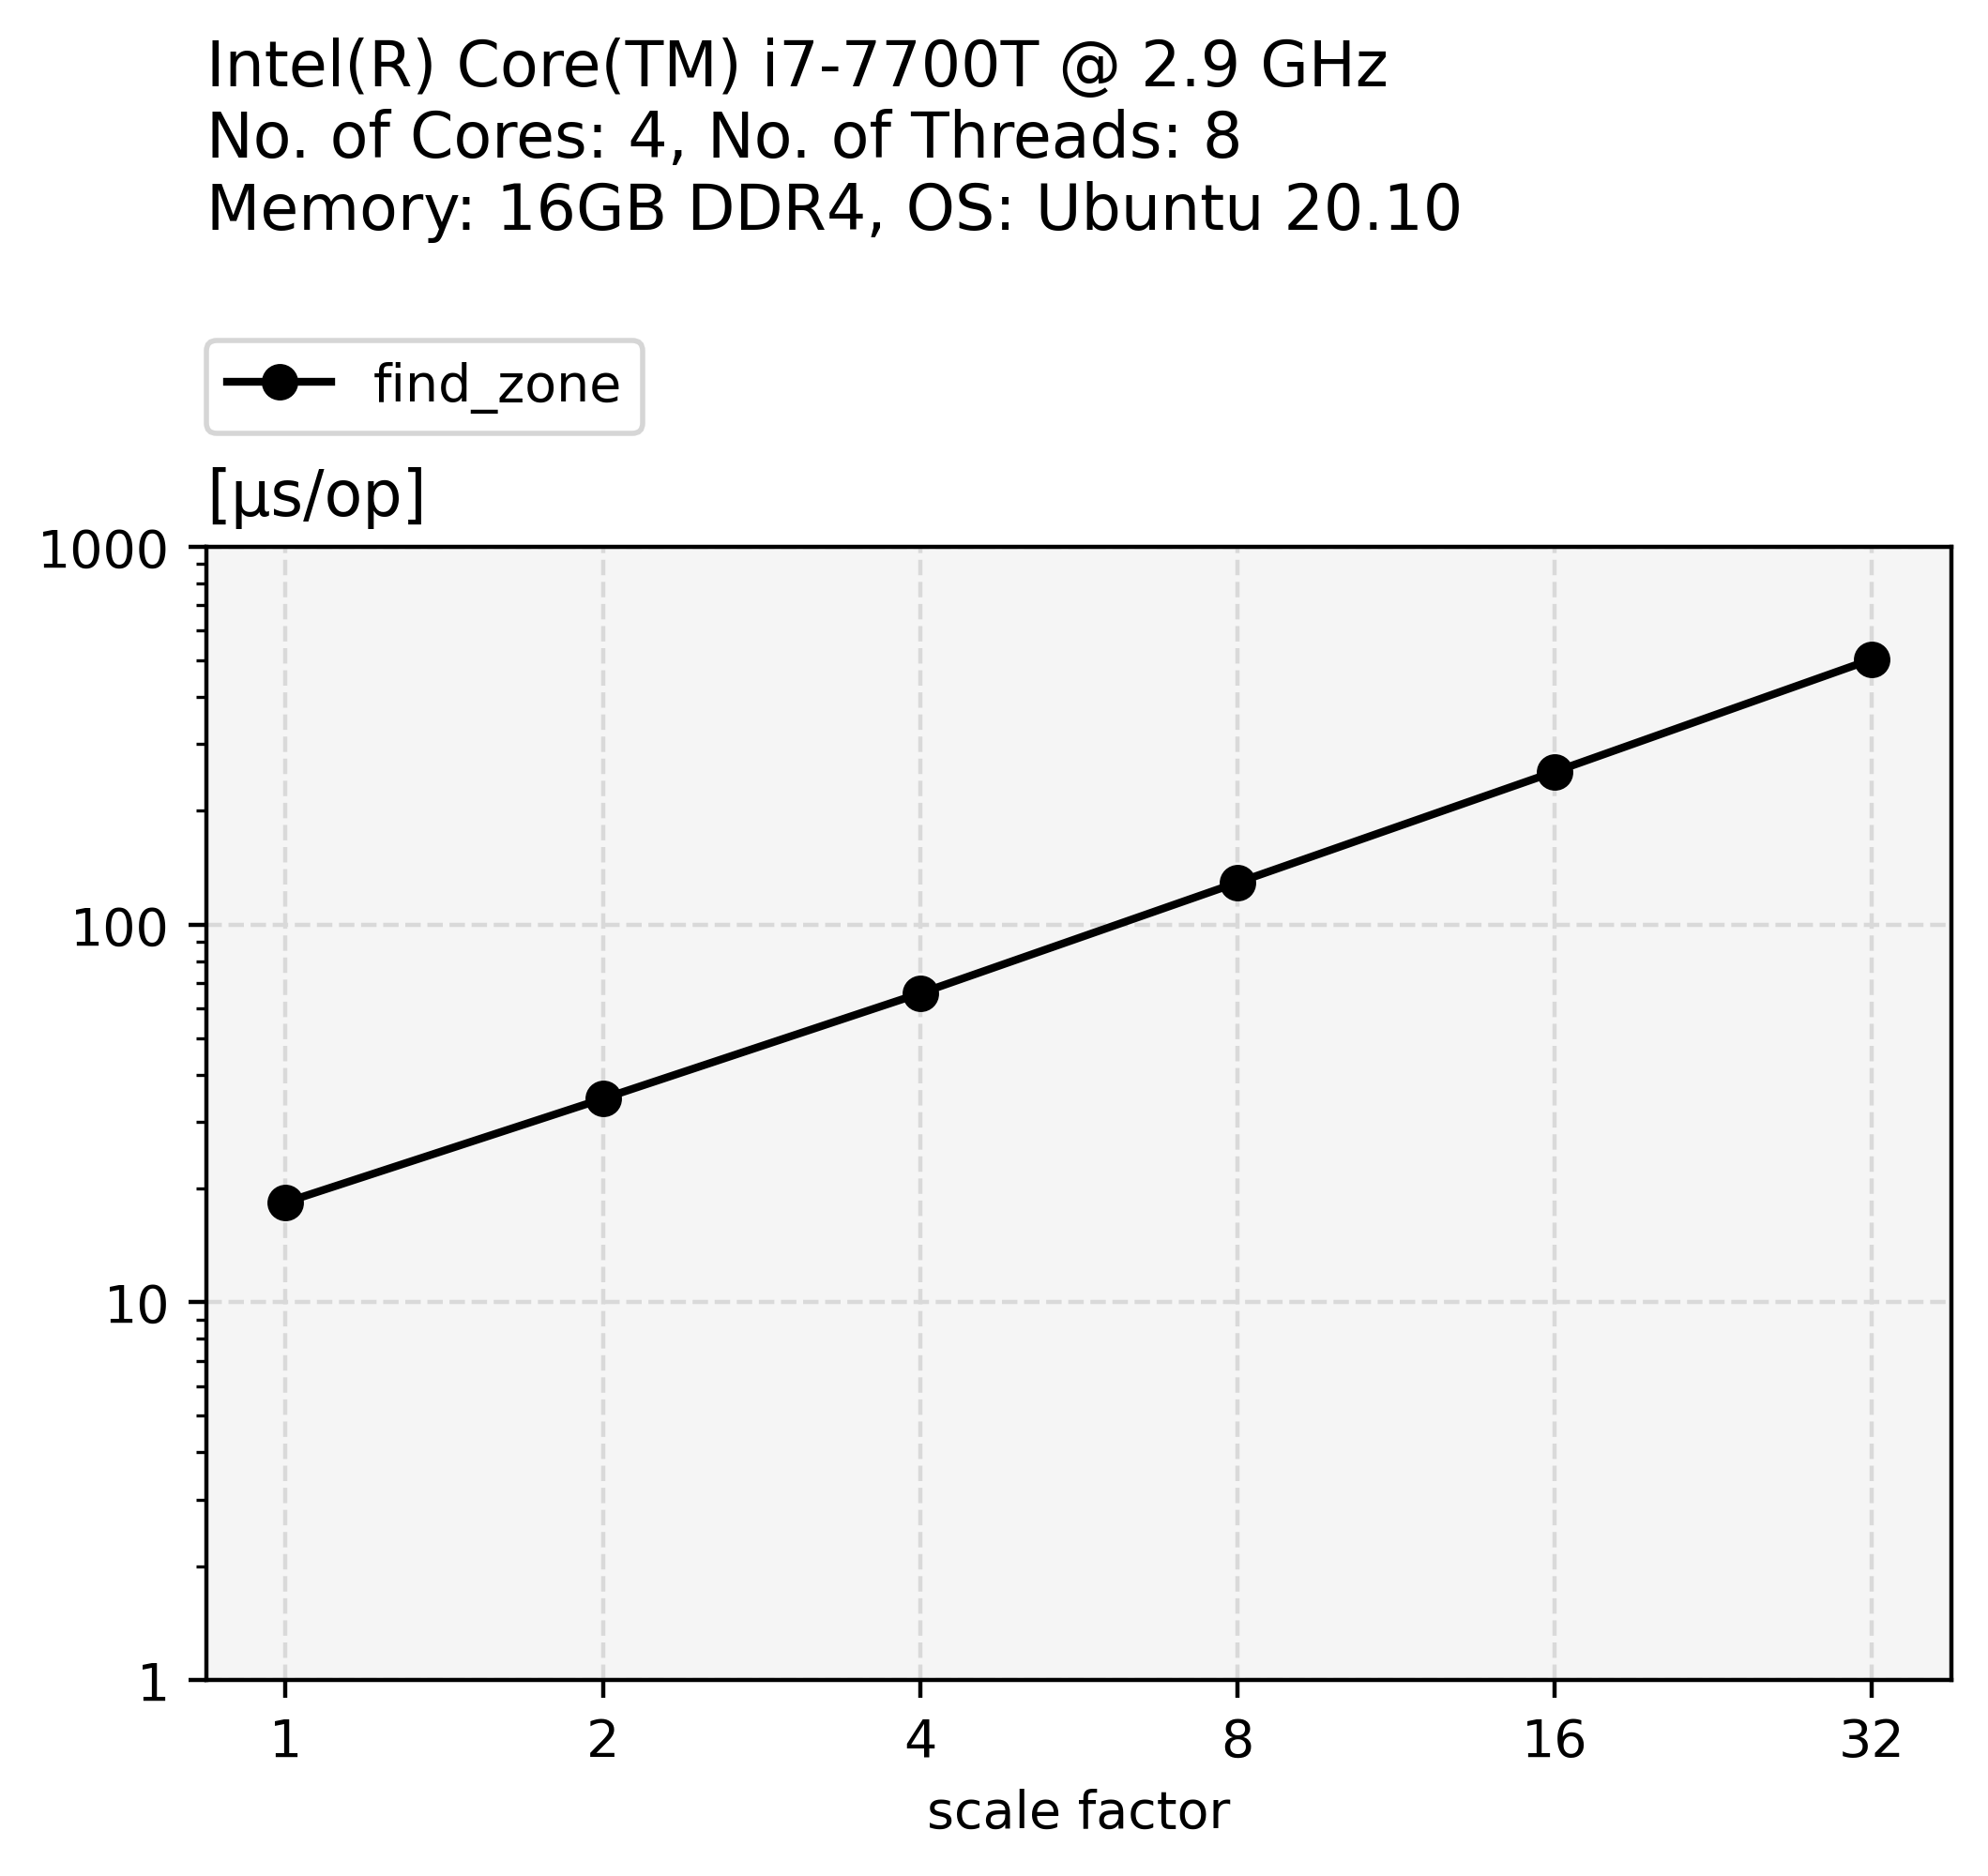
\includegraphics[width=\linewidth]{img/find_zone.png}
      \caption{\texttt{find\_zone} Function Scalability}
      \label{fig:sub: find zone Scalability}
    \end{subfigure}\hfill%
    \begin{subfigure}[t]{.22\textwidth}
      \centering
      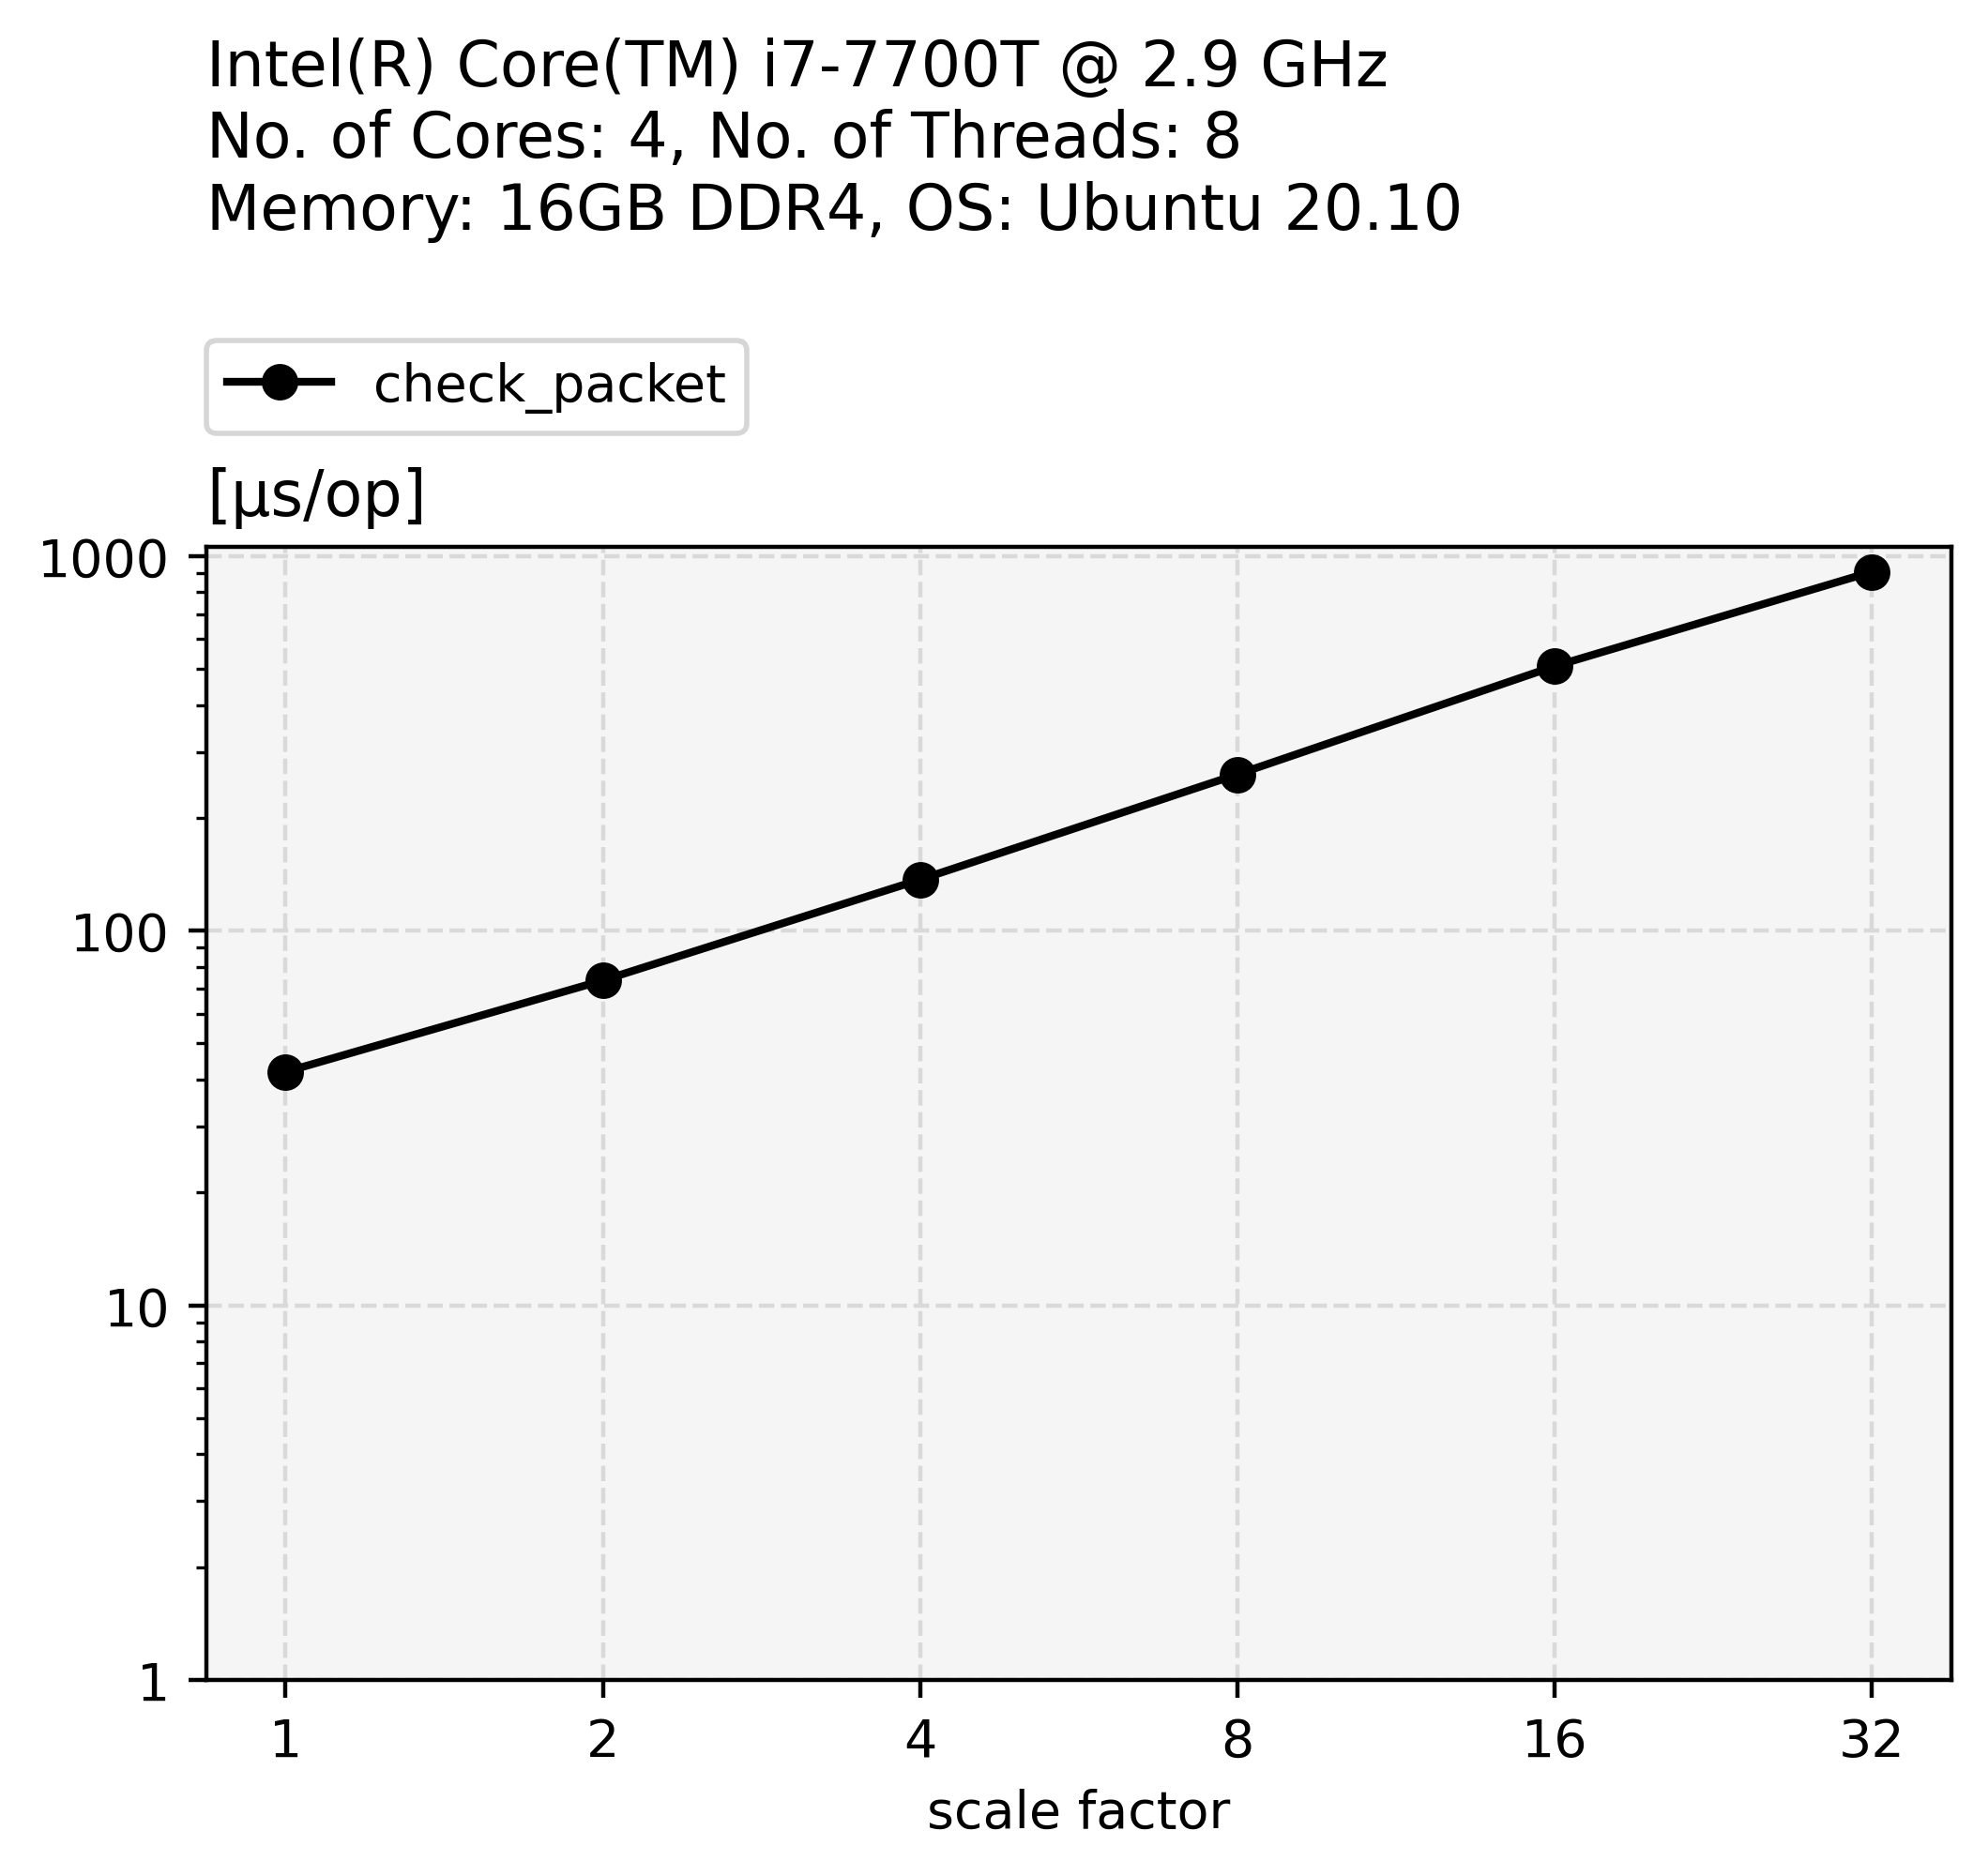
\includegraphics[width=\linewidth]{img/check_packet.png}
      \caption{\texttt{check\_packet} Function Scalability}
      \label{fig:sub: check packet Scalability}
    \end{subfigure}
    \caption{Endpoint \acs{TP} Scalability (Upscaling the number of subnets and policies)}
    \label{fig:Endpoint TP Scalability}
\end{figure}

\begin{figure}[t]
    \centering
    \begin{subfigure}[t]{.22\textwidth}
      \centering
      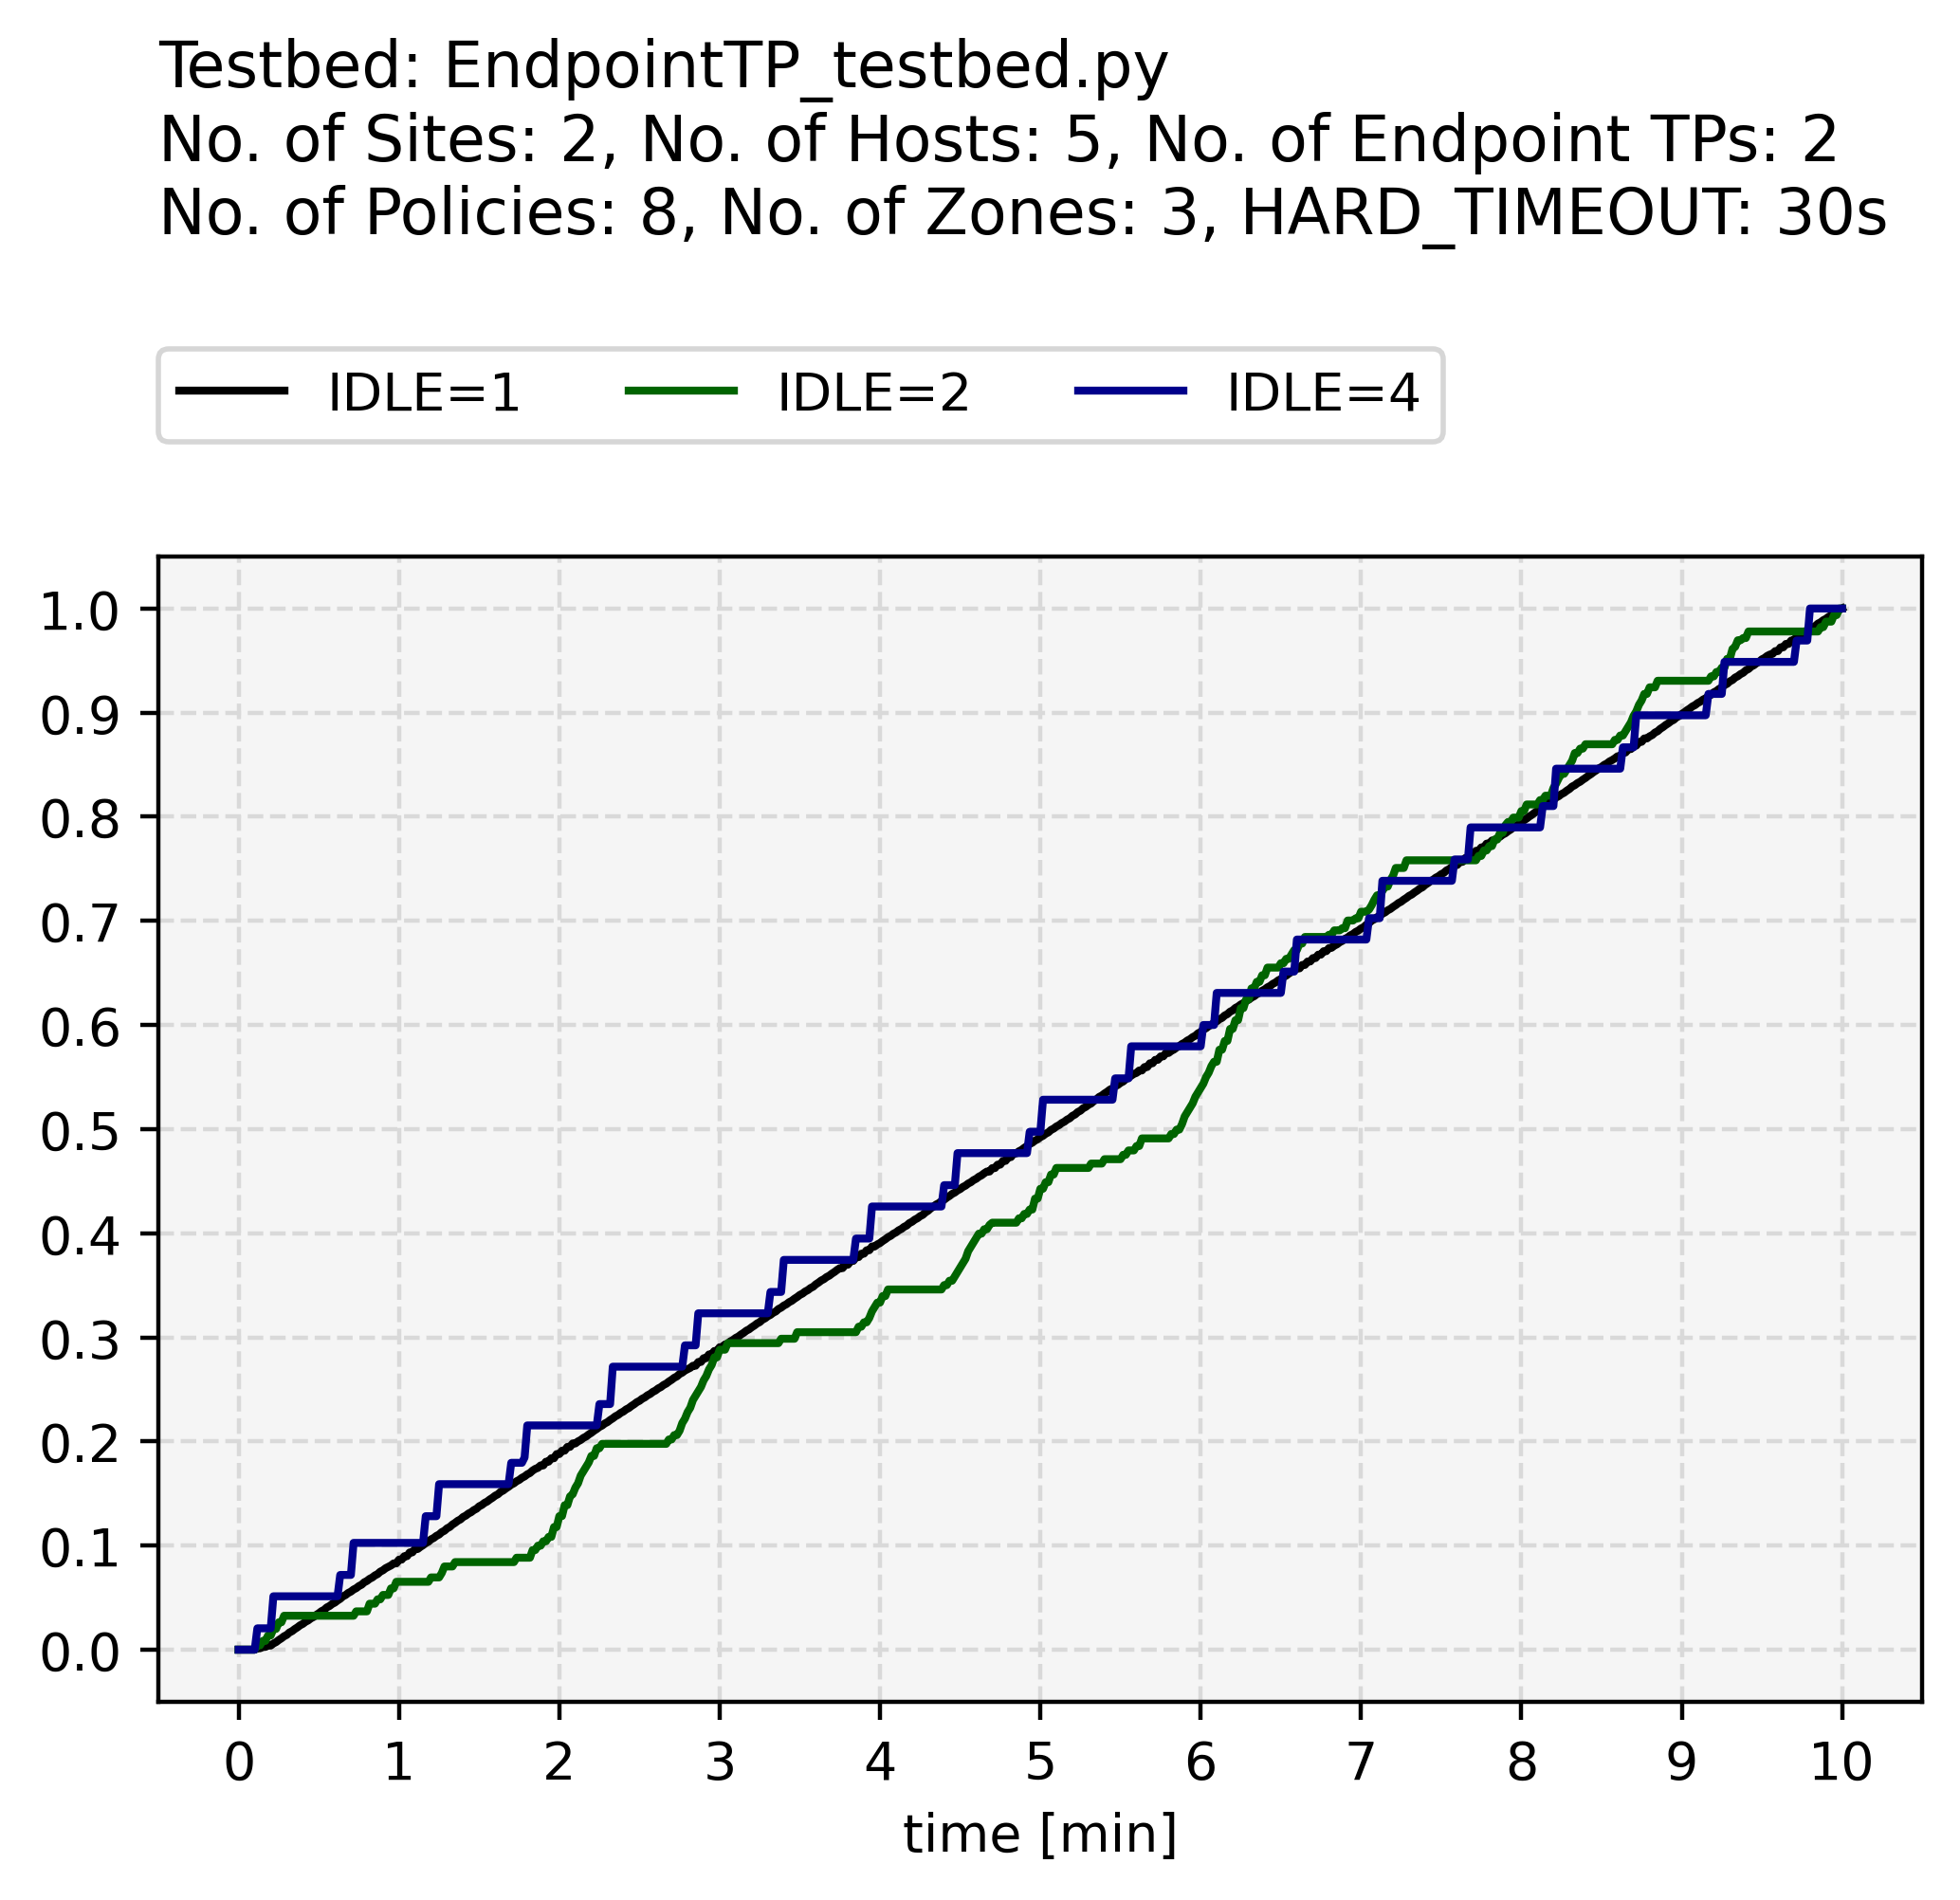
\includegraphics[width=\linewidth]{img/packet-in_idle_new_cdf.png}
      \caption{Varying \texttt{IDLE\_TIMEOUT}}
      \label{fig:sub: Varying IDLE_TIMEOUT}
    \end{subfigure}\hfill%
    \begin{subfigure}[t]{.22\textwidth}
      \centering
      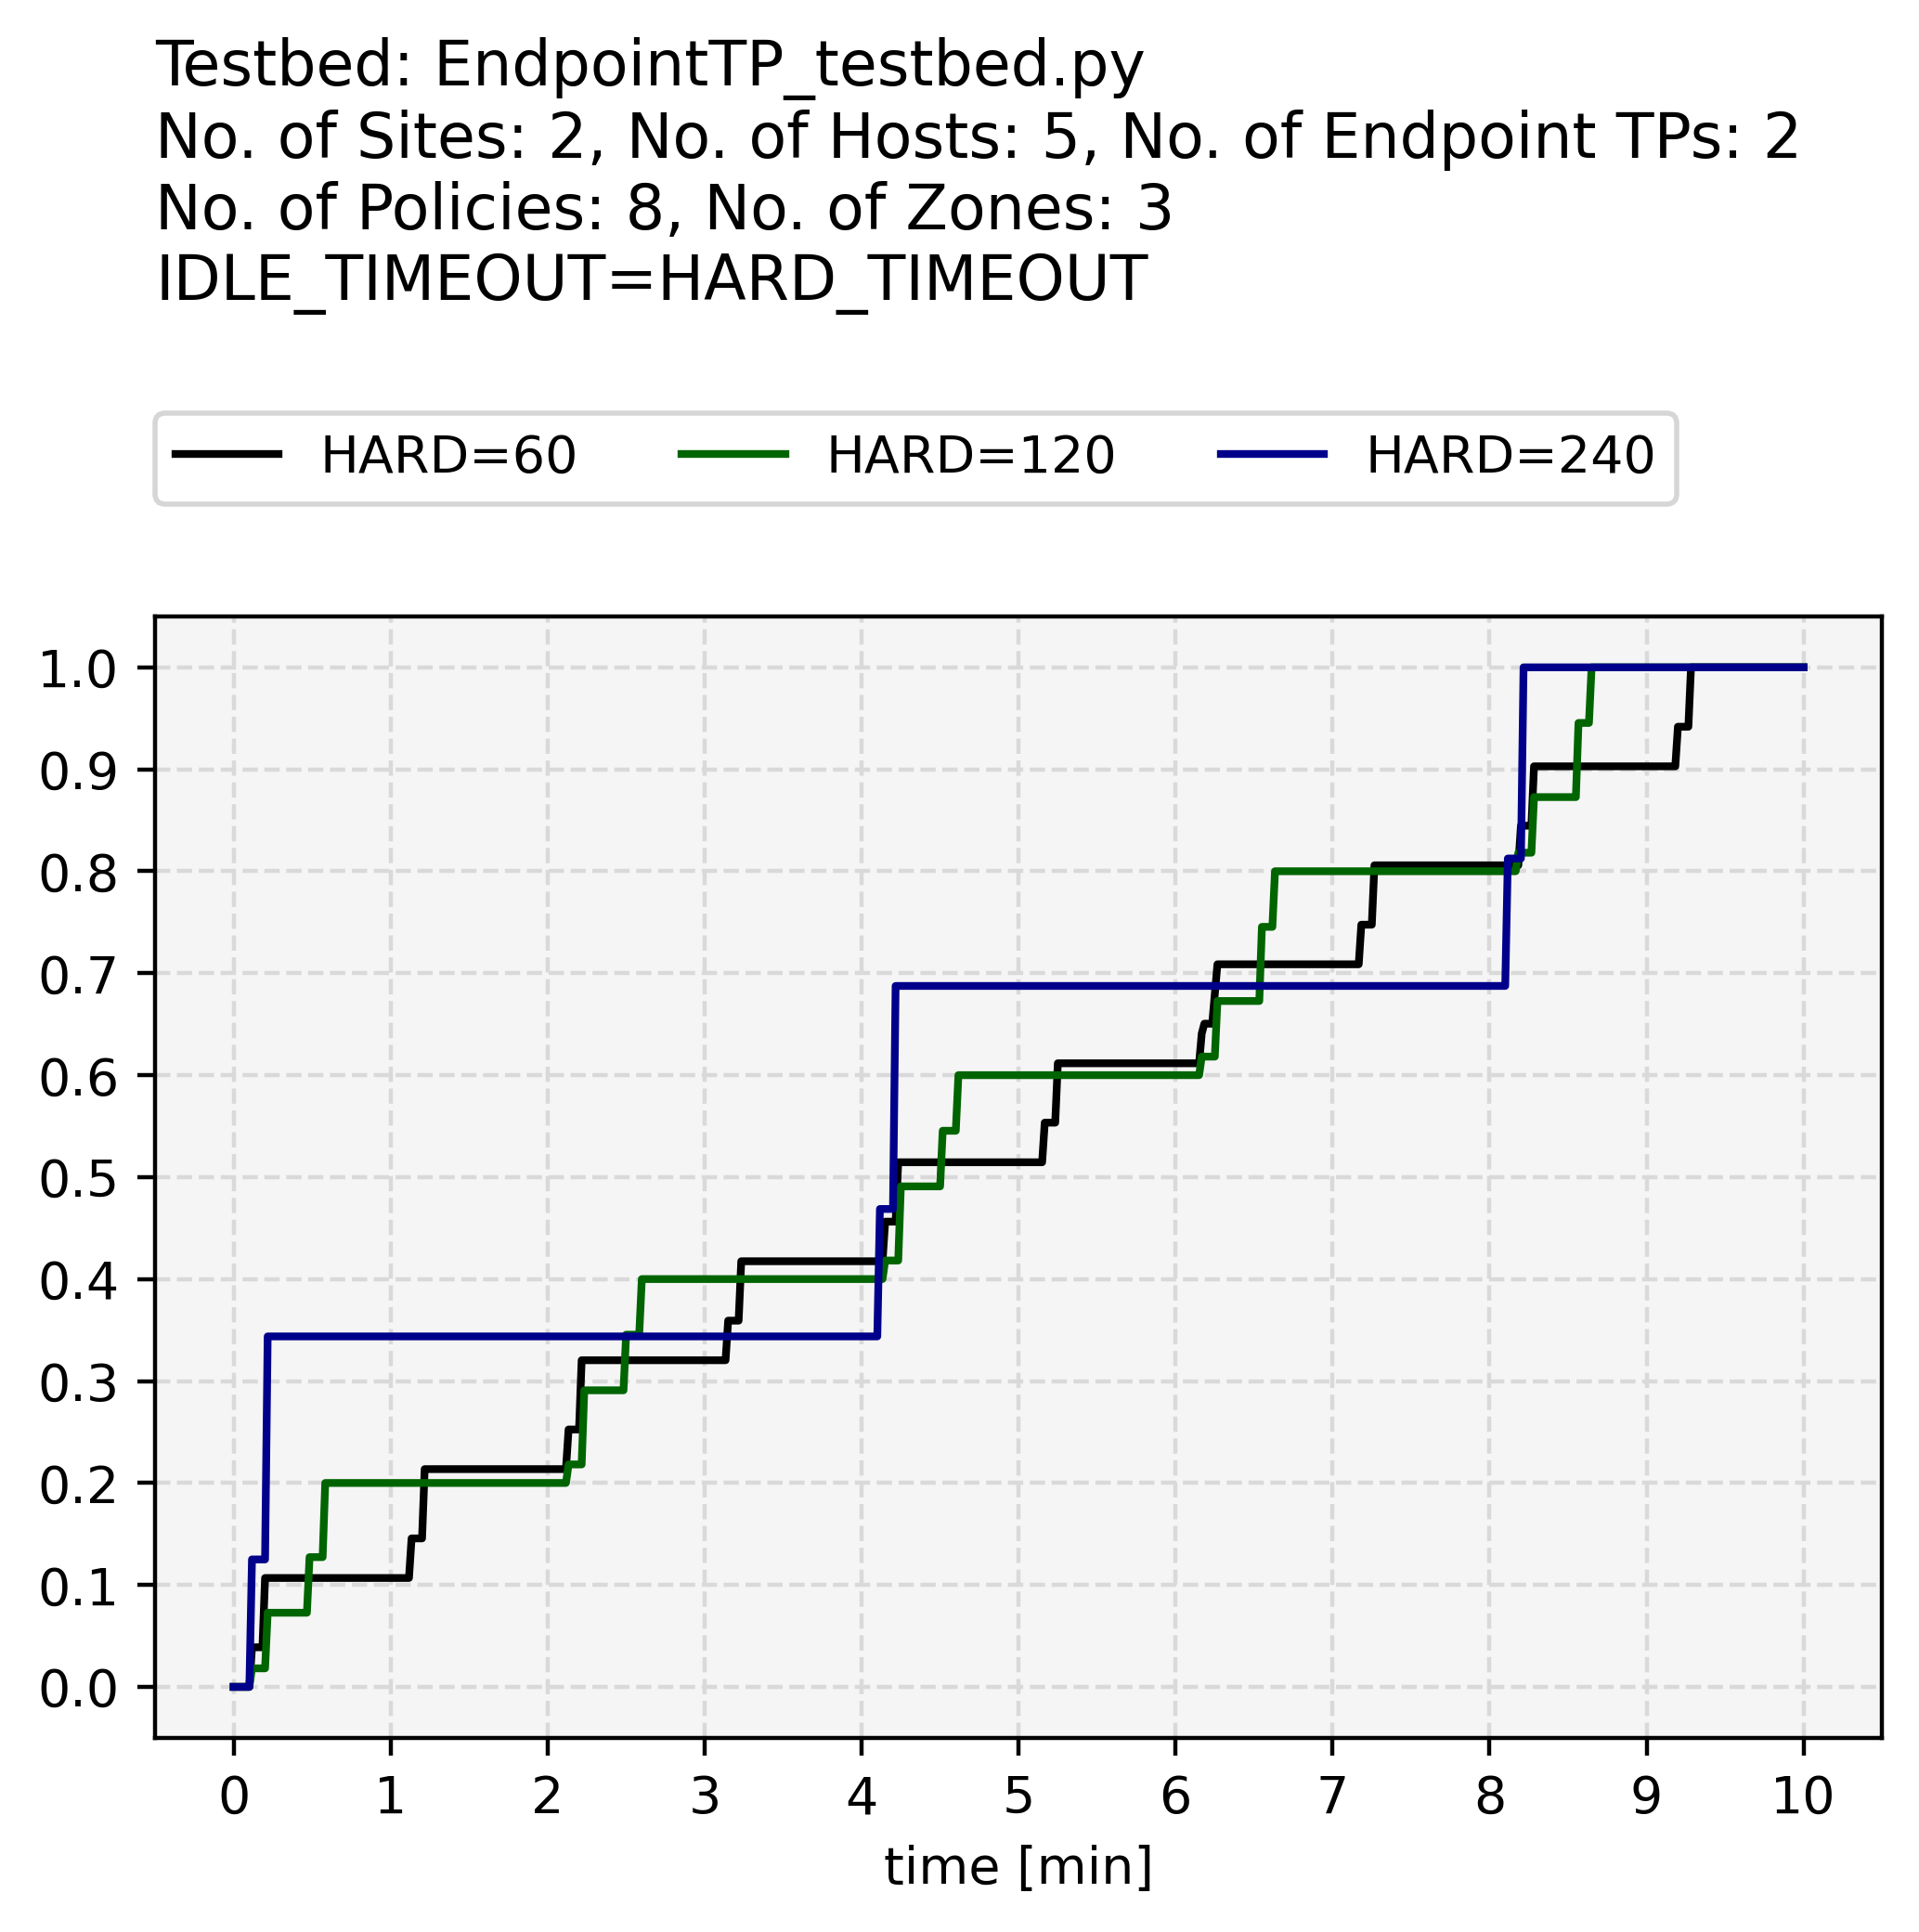
\includegraphics[width=\linewidth]{img/packet-in_hard_new_cdf.png}
      \caption{Varying \texttt{HARD\_TIMEOUT}}
      \label{fig:sub: Varying HARD_TIMEOUT}
    \end{subfigure}
    \caption{\acs{CDF} Plot of Packet-In Messages per Time (Sum of two instances of Endpoint \acsp{TP})}
    \label{fig:CDF Plot of Packet-In Messages per Time}
\end{figure}

Another factor that we should investigate when evaluating the performance of an Endpoint \acs{TP} is the workload it needs to be able to handle and what factors influence the magnitude of the workload. We measure the workload as the number of packet-in messages an Endpoint \acs{TP} needs to handle over time. Many factors, like the number of hosts, the type of traffic they generate, the complexity of the policy database or the presence of an attacker influence the workload. These factors are however hard to simulate and their effect can be controlled by scaling up or employing additional defense mechanisms, in case of an attacker being present. What however is of interest to us is how certain parameters we choose while deploying MONDRIAN affect the workload on the Endpoint \acs{TP}. For that we consider the two OpenFlow parameters \texttt{IDLE_TIMEOUT} and \texttt{HARD_TIMEOUT} and analyze how they should be chosen, depending on the desired properties a data center operator would like to achieve.

The \texttt{IDLE_TIMEOUT} should be chosen in a way, such that the flow table of an \acs{SDN} switch doesn't get exhausted. If a flow table is too full of flow table entries, then we should decrease the size of the \texttt{IDLE_TIMEOUT}. Otherwise, it's better to have an as big as possible \texttt{IDLE_TIMEOUT}, since we don't want to unnecessarily cause an \acs{SDN} switch to contact an Endpoint \acs{TP} only because a machine was inactive for some time. 

The \texttt{HARD_TIMEOUT} should also be chosen as big as possible, with the constraint that the \texttt{refresh_interval} of the Endpoint \acs{TP} added to the \texttt{HARD_TIMEOUT} doesn't exceed the responsiveness requirement to policy changes. The \texttt{HARD_TIMEOUT}'s responsibility is to make sure that flow table entries expire once they could be outdated.

In our experiment, we use the Endpoint \acs{TP} testbed with a traffic generator, which periodically lets all hosts of the same zone ping each other and then sleeps for two seconds to simulate idle time. With the \texttt{Stats} module we then measure the number of packet-in messages over a time period of 10 minutes.

In the \acs{CDF} (\acl{CDF}) plot in figure \ref{fig:sub: Varying IDLE_TIMEOUT} we show the results for \texttt{IDLE_TIMEOUT}s 1, 2 and 4 seconds. For \texttt{IDLE_TIMEOUT} = 1 we have a smooth line, meaning that we get a continuous stream of packet-in messages. This is because the timeout (1s) is smaller than the idle time (2s) we simulate. Hence, we get flow table misses in each round of the traffic generator. If the idle time (2s) is equal to the timeout (2s), we get a curvy line which isn't smooth nor spikey. This is because sometimes the idle time will be long enough to cause the flow table entries to be removed and sometimes it will be too short, depending on fluctuations in the performance of the testbed. If however the timeout (4s) is bigger than the idle time (2s), we get a sawtooth-shaped line with a step size of 30 seconds, which is the \texttt{HARD_TIMEOUT} in our experiment. This means that in this case the \texttt{IDLE_TIMEOUT} never had an effect, which is desirable for as long as the \acs{SDN} switches aren't exhausted. Like this we can determine the ideal \texttt{IDLE_TIMEOUT} for a specific kind of traffic. However, in our experiment we have artificially crafted traffic and real-world traffic can deviate arbitrarily from any artificially crafted traffic, making the choosing of ideal parameters a non-trivial problem. 

Figure \ref{fig:sub: Varying HARD_TIMEOUT} shows a \acs{CDF} plot where we vary the values for the \texttt{HARD_TIMEOUT} from 1 minute to 2 and 4 minutes. As we expect, all lines are sawtooth-shaped with the corresponding timeout length as a step size. Bigger steps, meaning bigger \texttt{HARD_TIMEOUT}s, mean that less packet-in messages will be received and are therefore desirable. However, as previously mentioned with increasing \texttt{HARD_TIMEOUT}s, we lower the responsiveness of the MONDRIAN deployment, which at some point might be inacceptable.

Conclusively, one can say that the \texttt{HARD_TIMEOUT} should be chosen as large as acceptable with regards to the responsiveness of the system, whereas the \texttt{IDLE_TIMEOUT} should be chosen as large as possible for as long as no \acs{SDN} switches are exhausted. Overall, with reasonably chosen parameters, the Endpoint \acs{TP} will for sure be performant enough to not be the performance bottleneck on the data path.

%\todo{\\
%    - Performance good due to Openflow switches \\
%    - Get measurements and discuss them here (packet-in msg per workload depending on some parameters)\\
%    - Result: Performance is good meaning it won't be the bottleneck
%}

\FloatBarrier
\subsubsection{Gateway TP}
The Gateway \acs{TP} is much more performance critical, since it has to process every single packet, which is intended for a host in a different domain. We are mainly interested in the throughput and the latency of the Gateway \acs{TP} and in locating the performance bottlenecks.

Figure \ref{fig:Performance of MONDRIAN Conversion Functions} shows both the time a conversion to and from a MONDRIAN packet takes, as well as the throughput of these conversion functions. We can see that the \texttt{FromMondrian} operation is about 1.2x faster than the \texttt{ToMondrian} operation and has an approximately 2.5x higher throughput than its counterpart. The reason, why the \texttt{FromMondrian} operation is considerably more performant, is that the MONDRIAN packet carries all information used for the transformation already in the header, while the gathering of this information in the \texttt{ToMondrian} operation is costly, especially since it involves parsing and serializing more data. In general, these memory intensive gopacket operations are the major performance bottleneck as we can see if we optimize the conversion operations, such that we can avoid some of these operations.

As shown in figure \ref{fig:Performance Improvement in ToMondrianAndSend} and \ref{fig:Performance Improvement in FromMondrianAndSend}, we can achieve a speedup of 1.72x and 1.85x in the functions \texttt{ToMondrianAndSend} and \texttt{FromMondrianAndSend} respectively, by avoiding to serialize a buffer into a gopacket, just to then read out the buffer of the packet in order to send it in the sending process.

The fact that such a simple gopacket related optimization causes a significant speedup, is a strong indicator that the gopackets are a major performance bottleneck. By analyzing the code with the Go profiler called \texttt{pprof}, we can see that apart from the gopacket related inefficiencies the next severe performance bottlenecks are the cryptographic operations. This was to be expected and is also good news since both of the aforementioned inefficiencies will naturally be avoided in production level code, since there we would be using more performant frameworks such as \acs{DPDK}, which minimizes the number of copying operations and has support for hardware accelerated cryptographic operations.

Conclusively, we can say that the benchmarking results are acceptable for a \acs{PoC} implementation, where fast prototyping was more important than the ability to write production level code. Furthermore, the design of the Gateway \acs{TP} is very minimalistic, which means that a production level implementation is expected to be able to compete performance wise with other commercial products in the same field such as \acs{VPN} solutions. 

%\todo{\\
%    - Microbenchmarking different functions \\
%    - Two performance penalties 1. gopackets 2. crypto -- both can be resolved in production level code with for example using DPDK \\
%    - Result: POC implementation shows limited performance due to gopackets/pcap but 
%    it can be implemented using DPDK and compete with commercial alternatives 
%    (Not done because too complicated for POC implementation -- fast prototyping was more important)
%}

\begin{figure}[t]
    \centering
    \begin{subfigure}[t]{.22\textwidth}
      \centering
      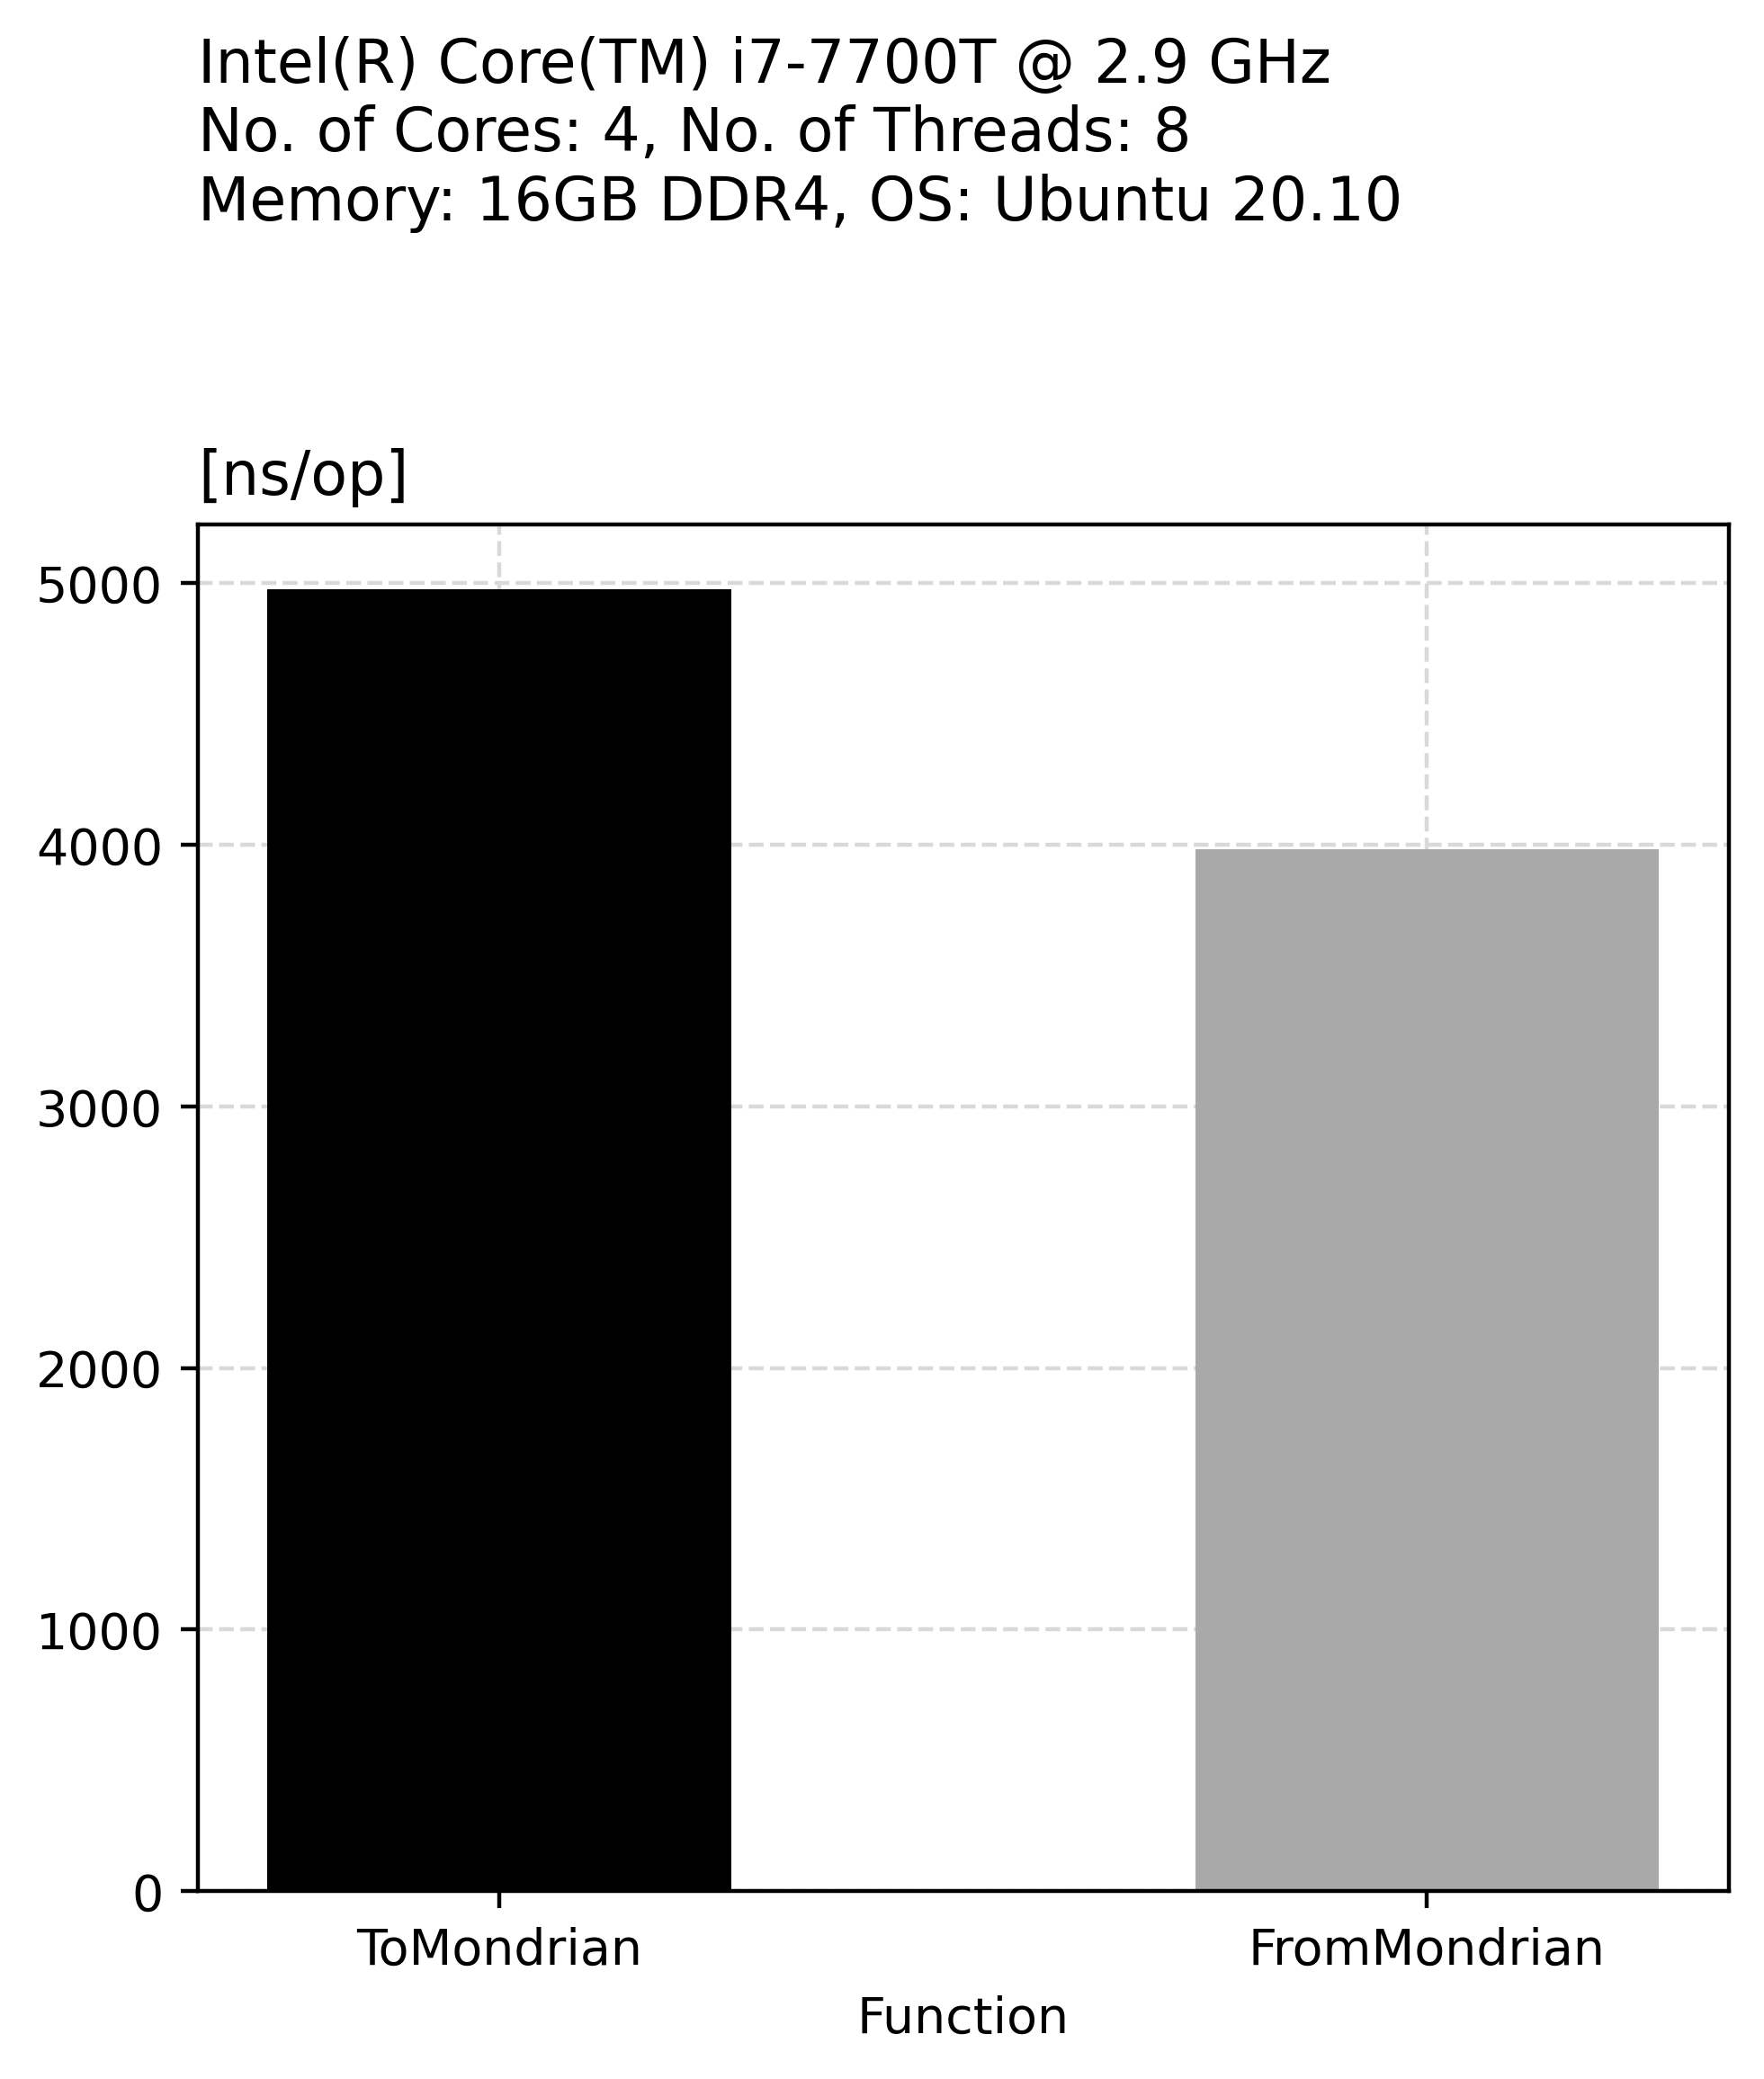
\includegraphics[width=\linewidth]{img/mondrian_transform_time.png}
      \caption{Time per Operation}
      \label{fig:sub: Time per Operation}
    \end{subfigure}\hfill%
    \begin{subfigure}[t]{.22\textwidth}
      \centering
      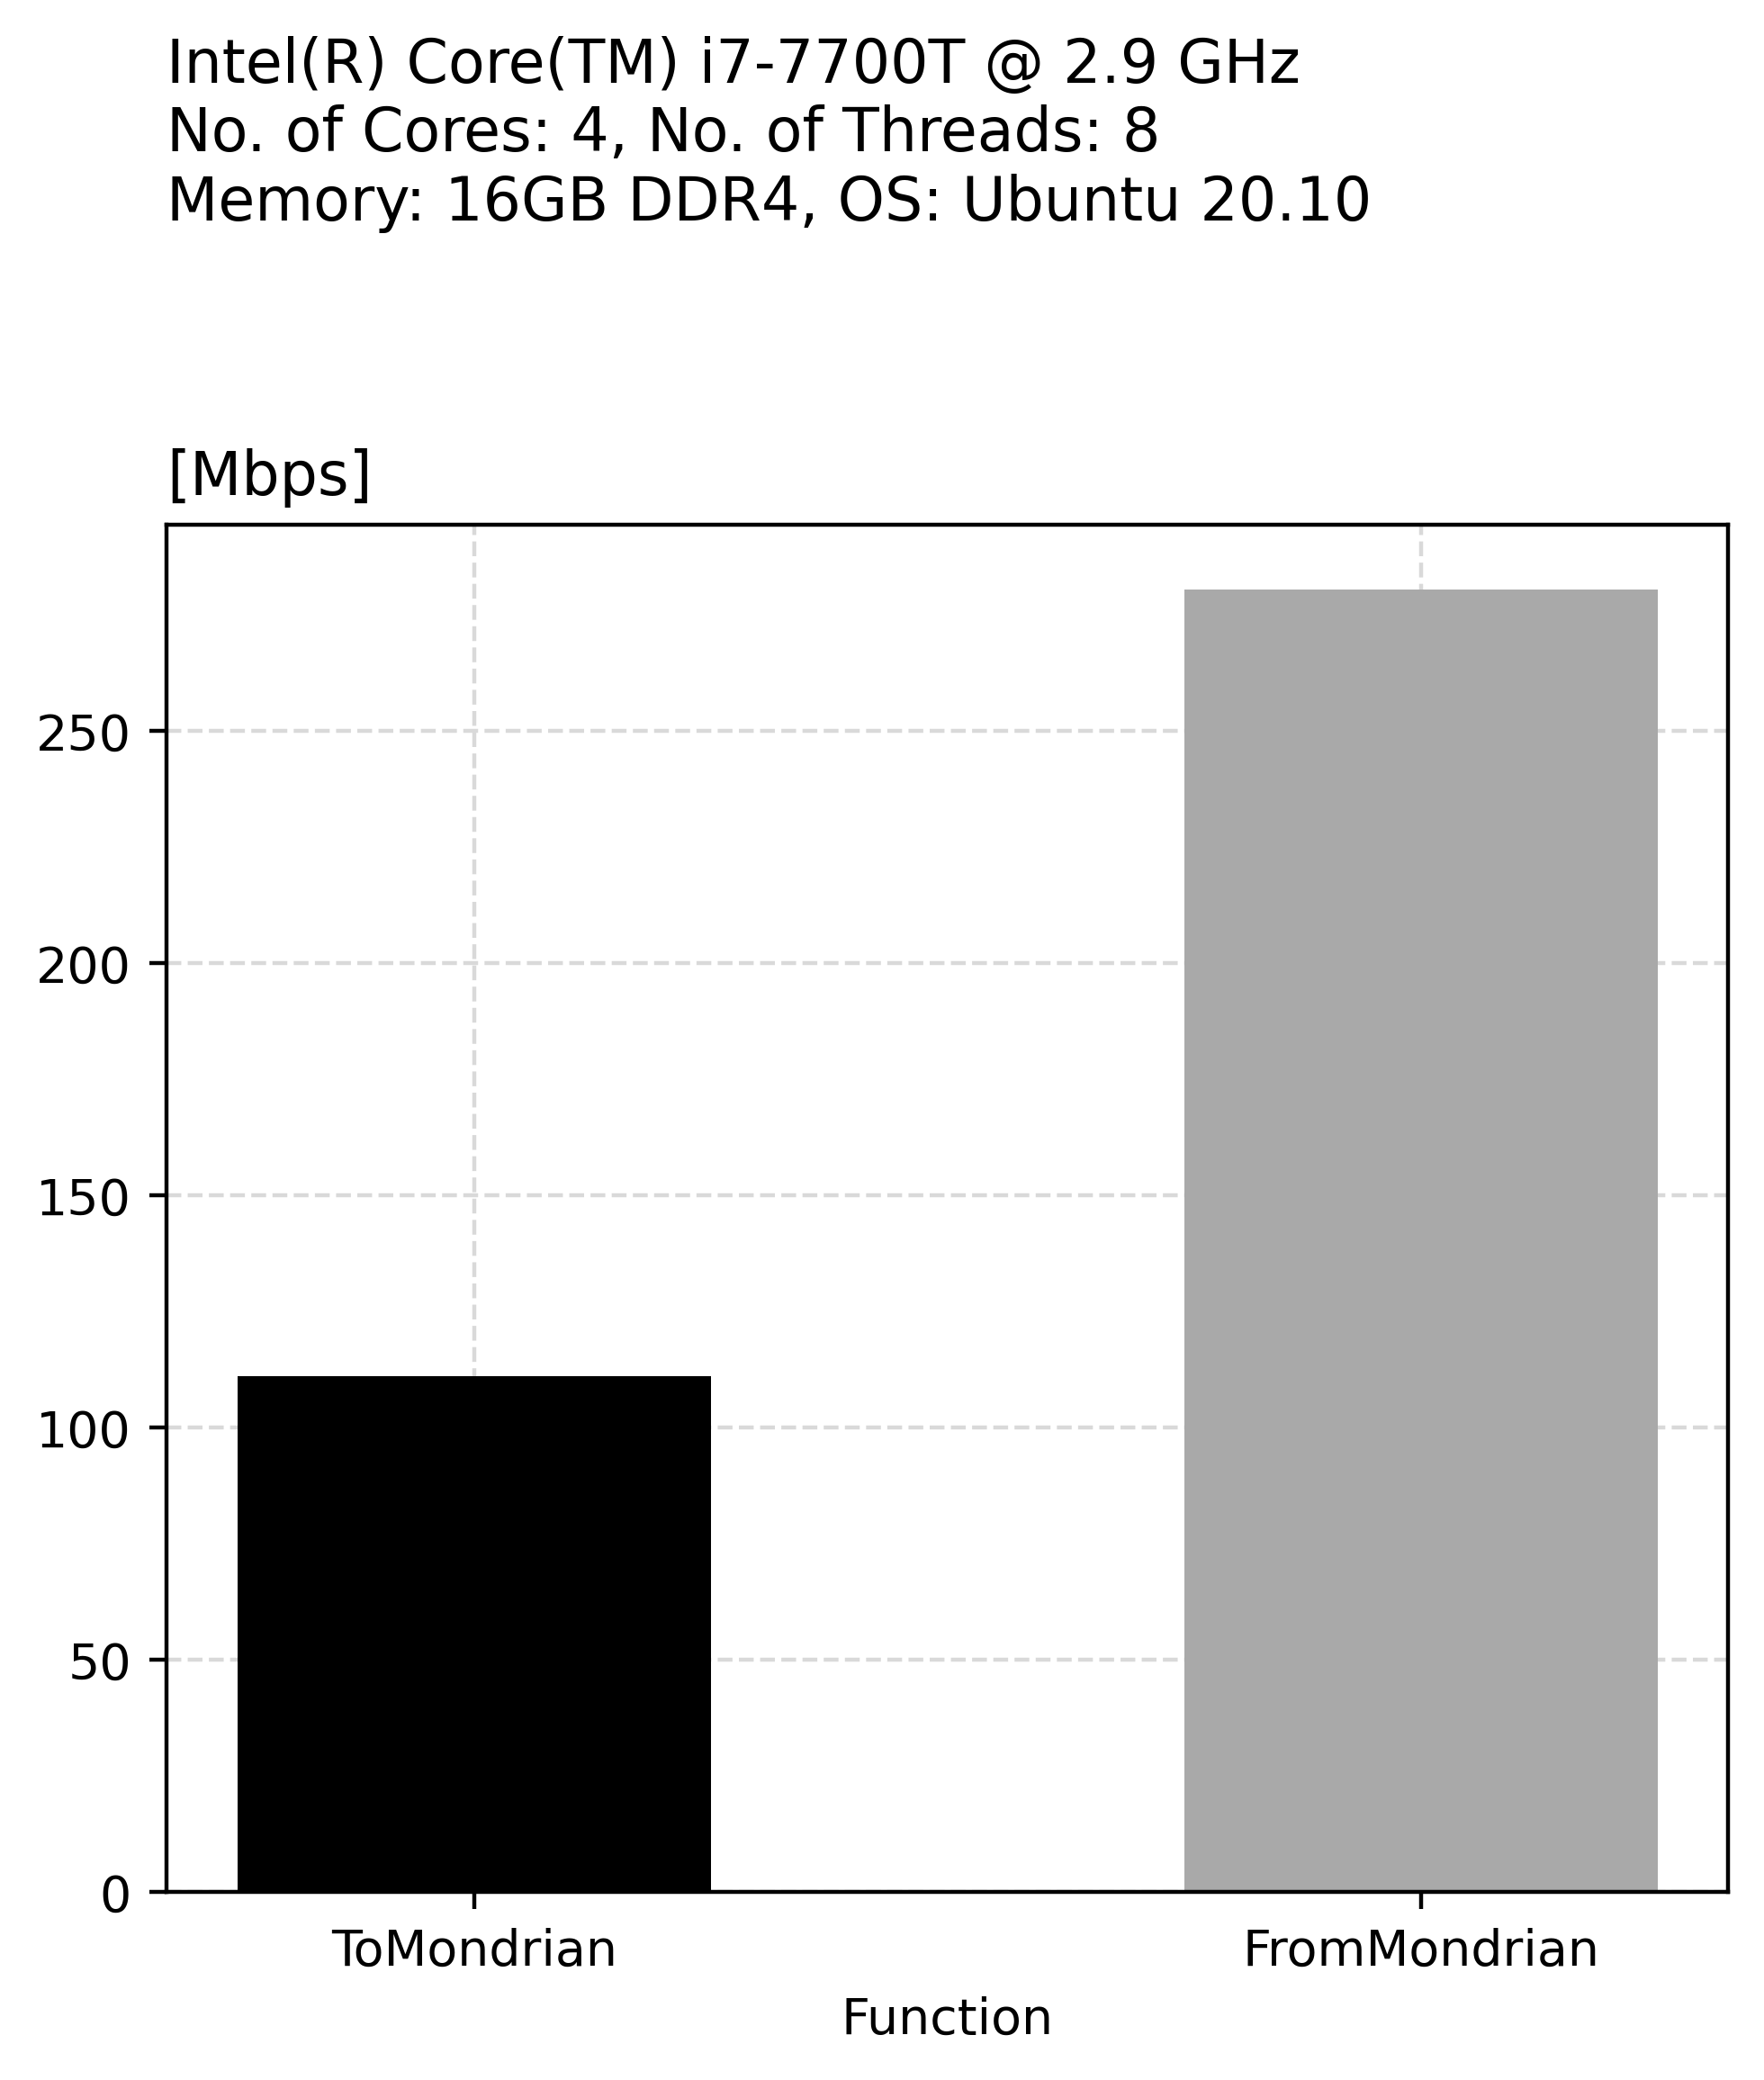
\includegraphics[width=\linewidth]{img/mondrian_transform_throughput.png}
      \caption{Throughput per Operation}
      \label{fig:sub: Throughput per Operation}
    \end{subfigure}
    \caption{Microbenchmarking Results of the MONDRIAN Conversion Functions}
    \label{fig:Performance of MONDRIAN Conversion Functions}
\end{figure}

\begin{figure}[t]
    \centering
    \begin{subfigure}[t]{.22\textwidth}
      \centering
      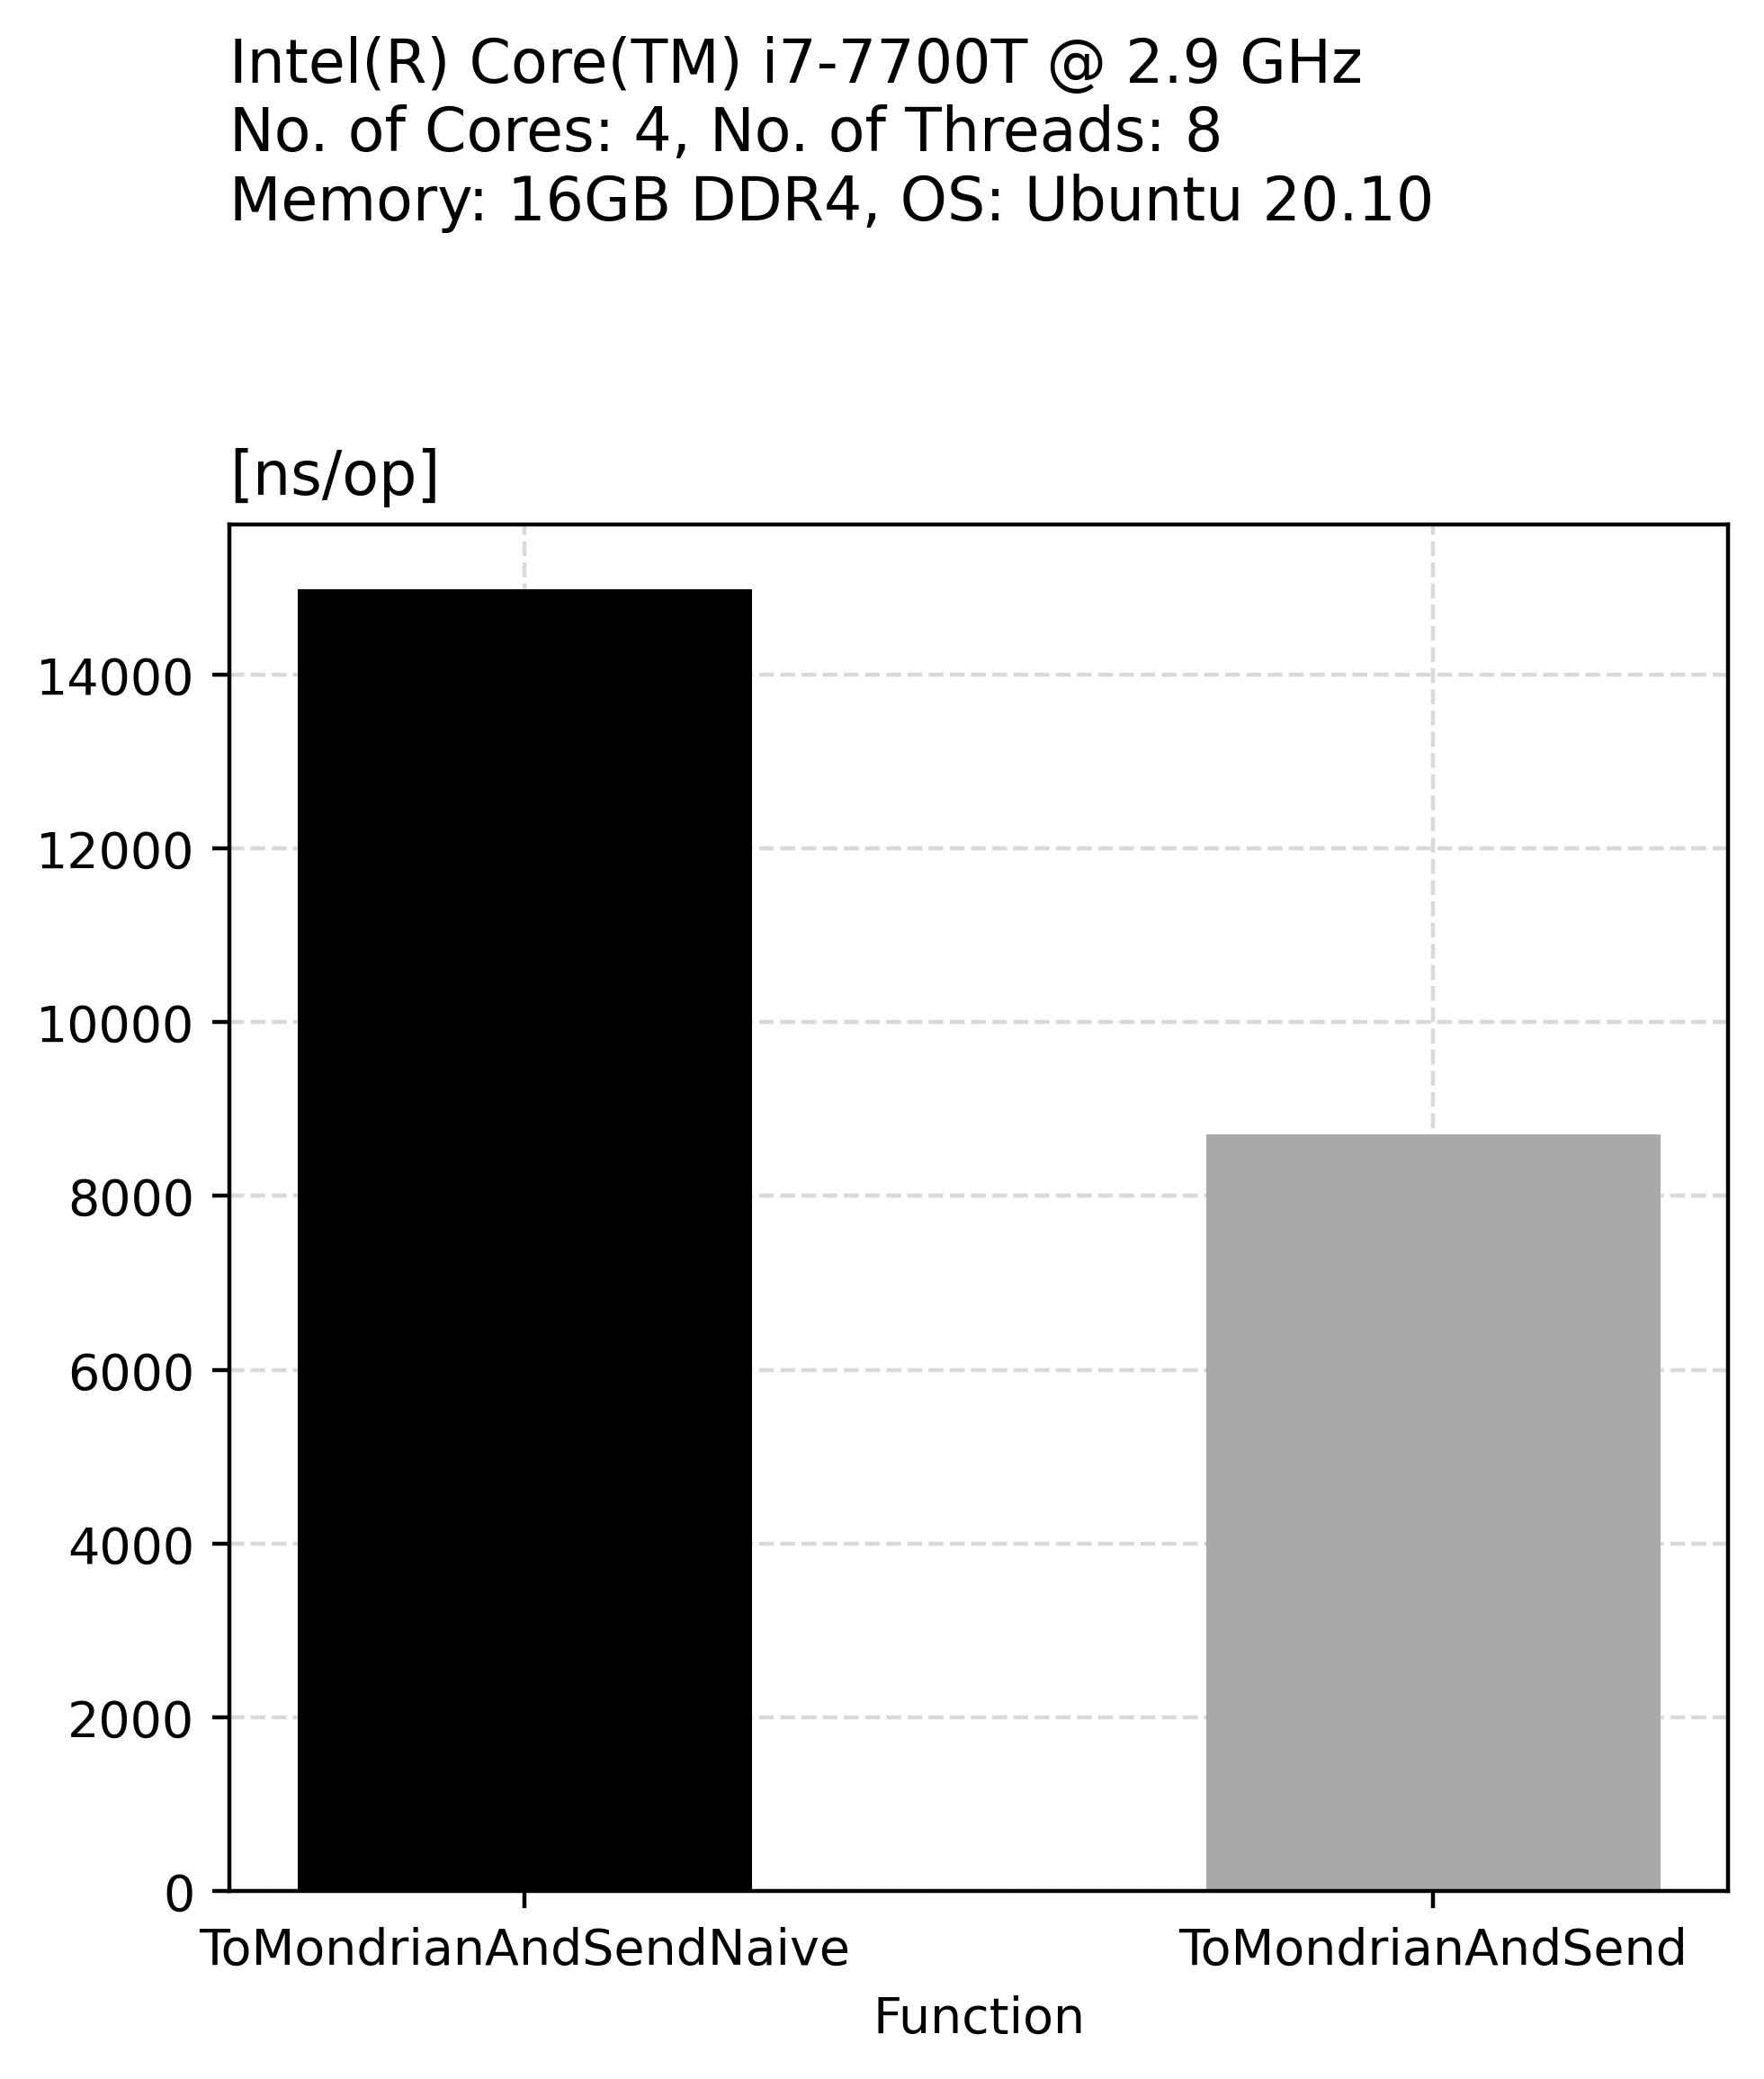
\includegraphics[width=\linewidth]{img/to_mondrian_and_send_opt_time.png}
      \caption{Latency Improvement}
      \label{fig:sub: Latency Improvement}
    \end{subfigure}\hfill%
    \begin{subfigure}[t]{.22\textwidth}
      \centering
      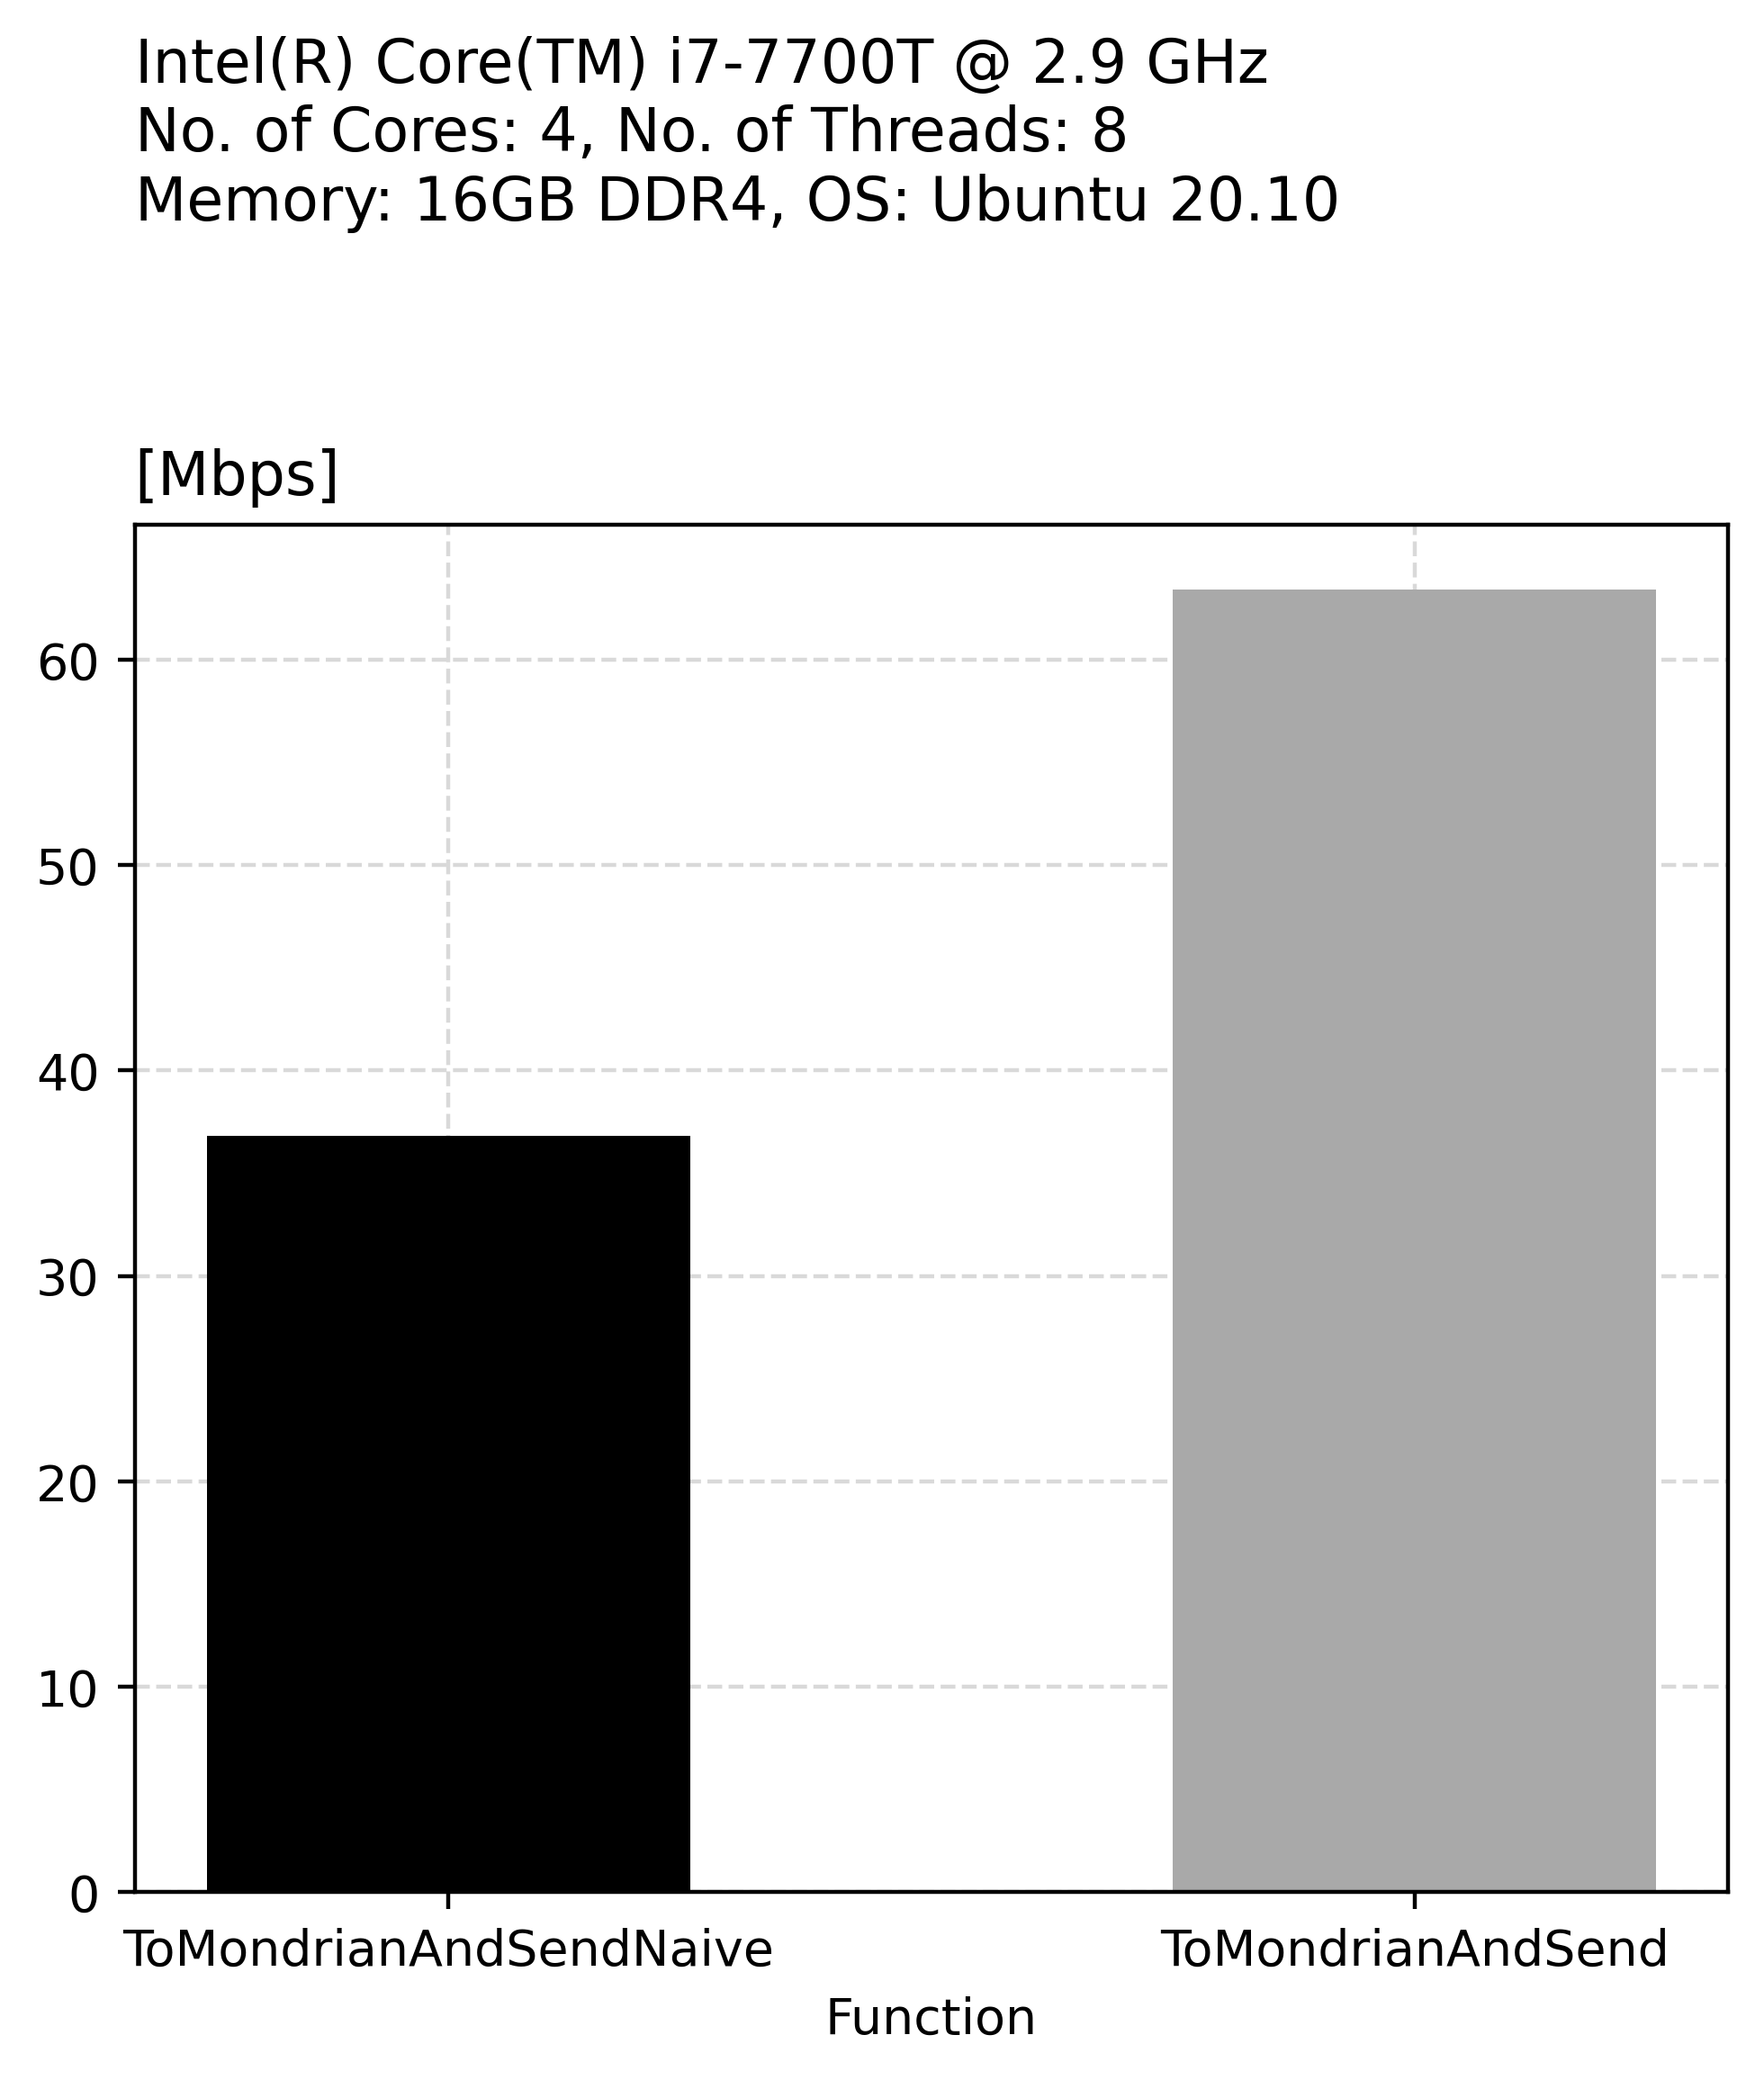
\includegraphics[width=\linewidth]{img/to_mondrian_and_send_opt_throughput.png}
      \caption{Throughput Improvement}
      \label{fig:sub: Throughput Improvement}
    \end{subfigure}
    \caption{Microbenchmarking Results of the Performance Improvement in \texttt{ToMondrianAndSend} (thanks to \texttt{gopacket} related optimizations)}
    \label{fig:Performance Improvement in ToMondrianAndSend}
\end{figure}

\begin{figure}[t]
    \centering
    \begin{subfigure}[t]{.22\textwidth}
      \centering
      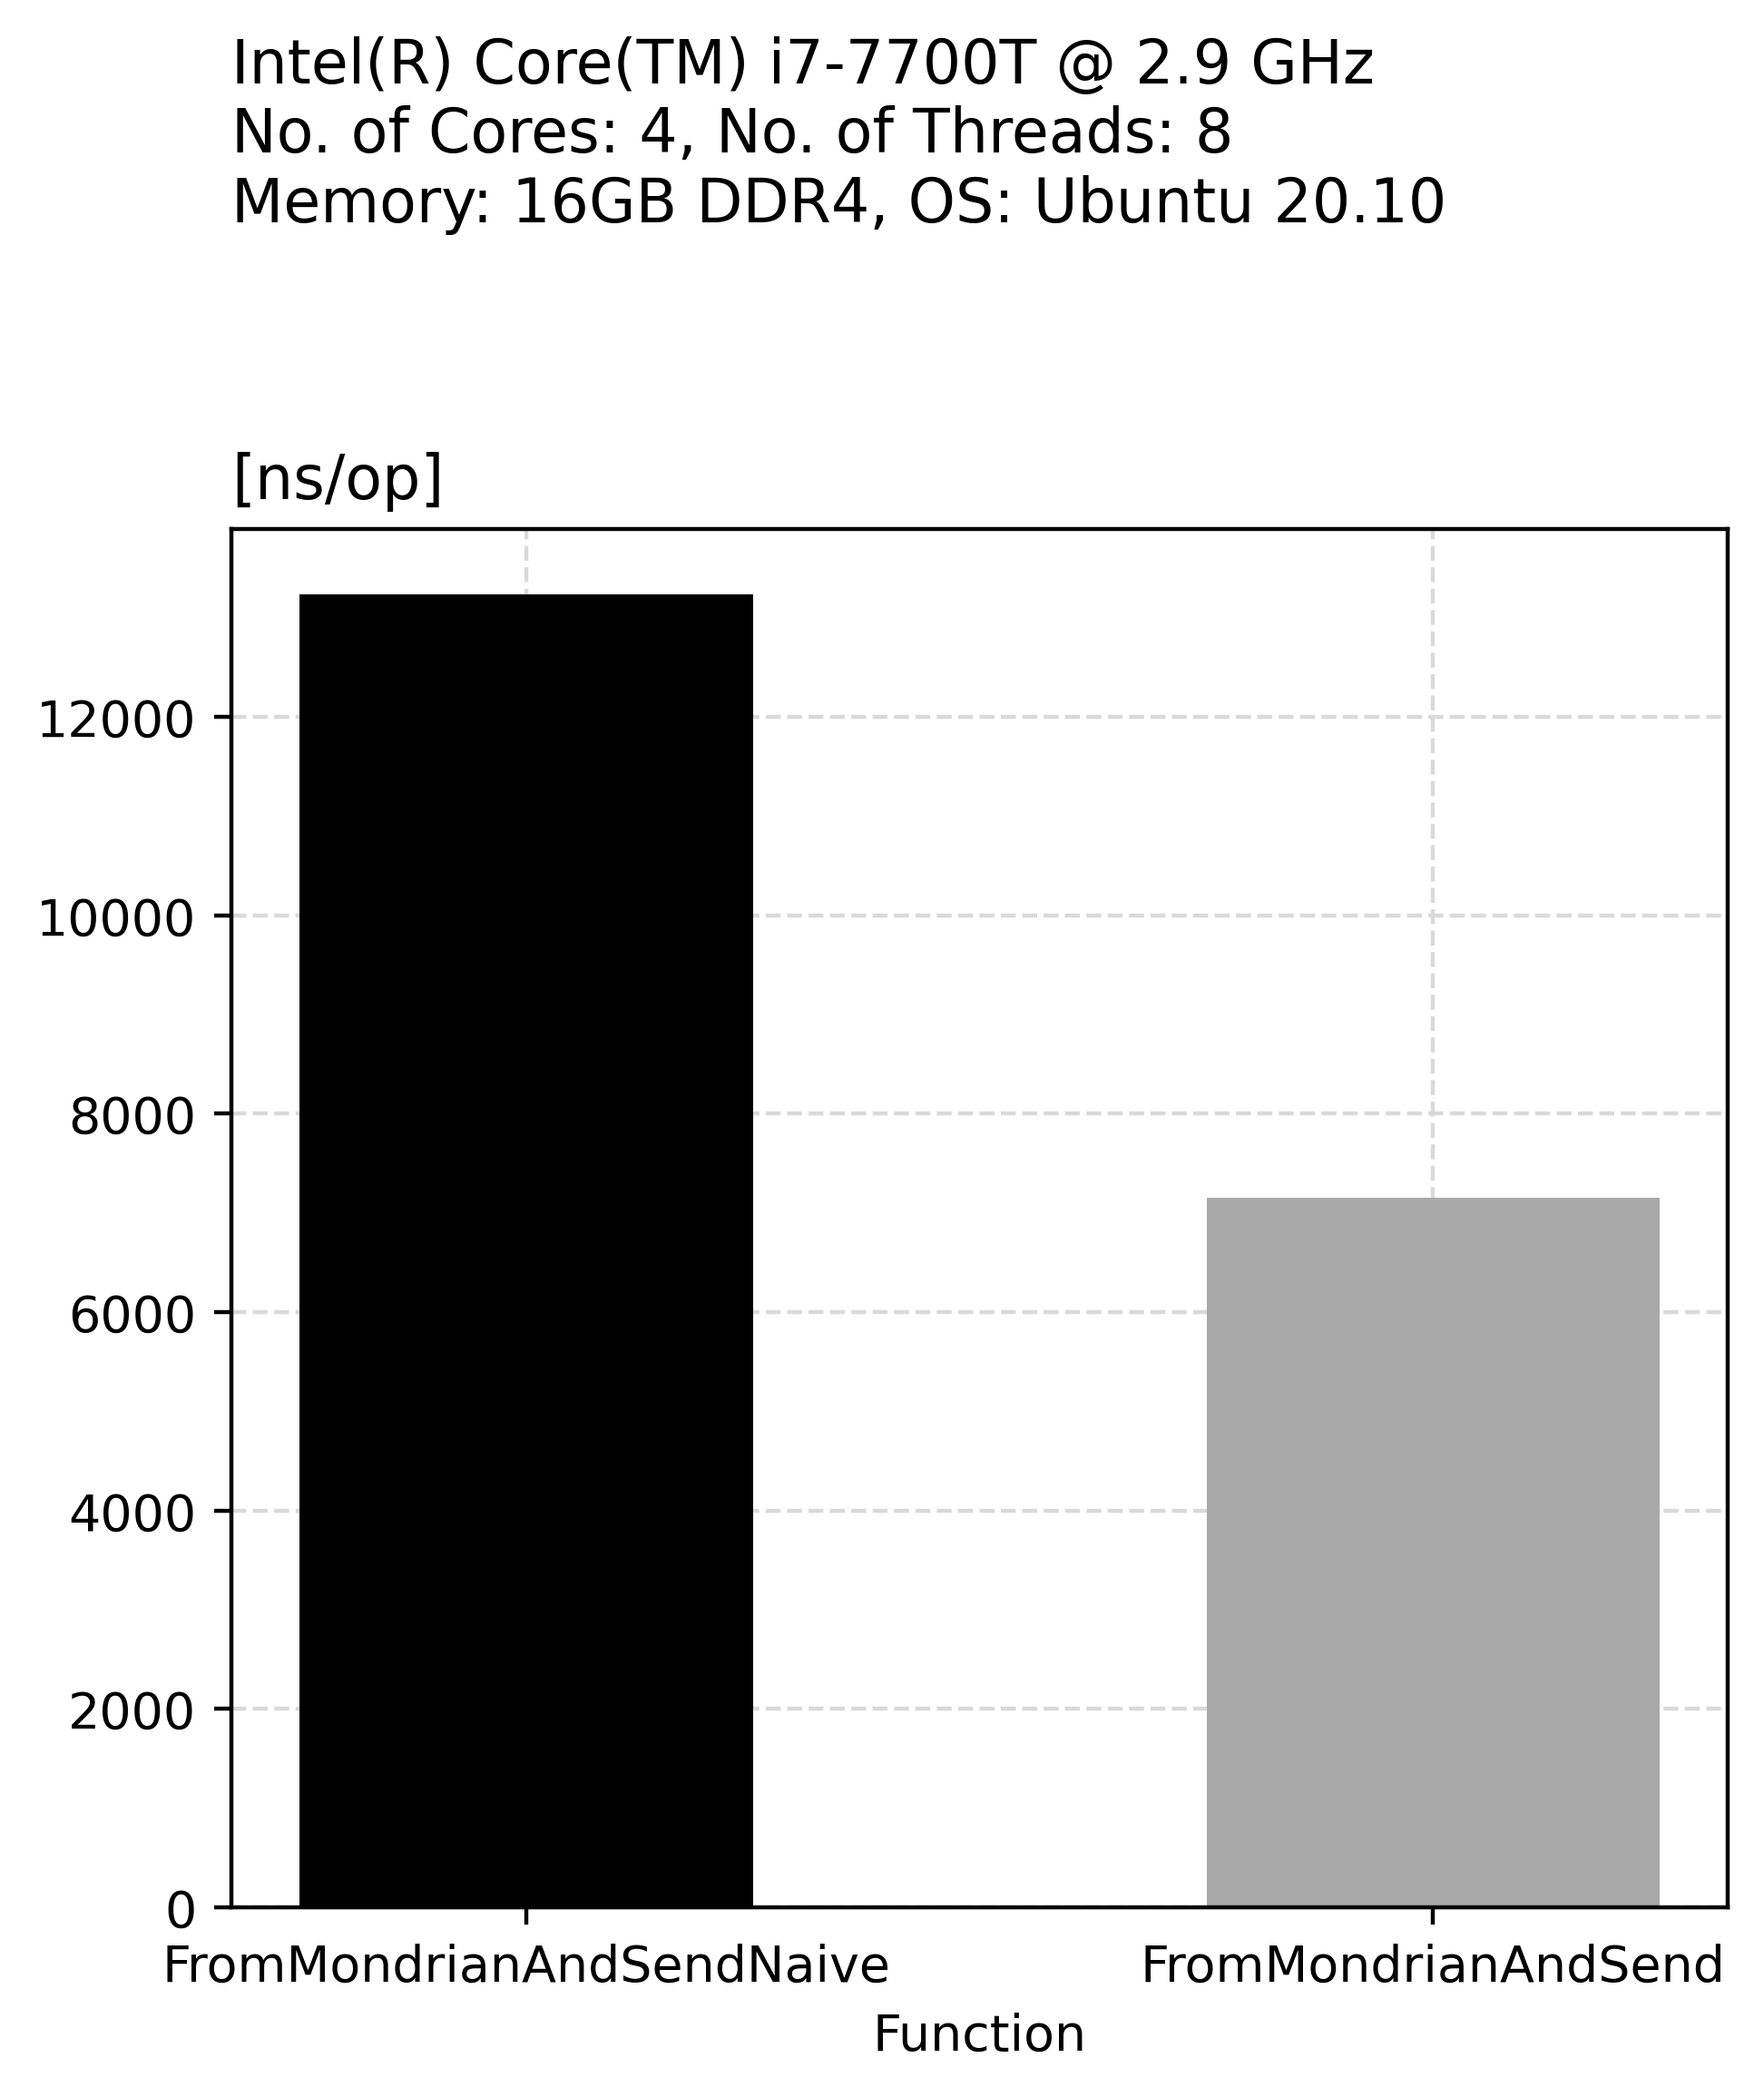
\includegraphics[width=\linewidth]{img/from_mondrian_and_send_opt_time.png}
      \caption{Latency Improvement}
      \label{fig:sub2: Latency Improvement}
    \end{subfigure}\hfill%
    \begin{subfigure}[t]{.22\textwidth}
      \centering
      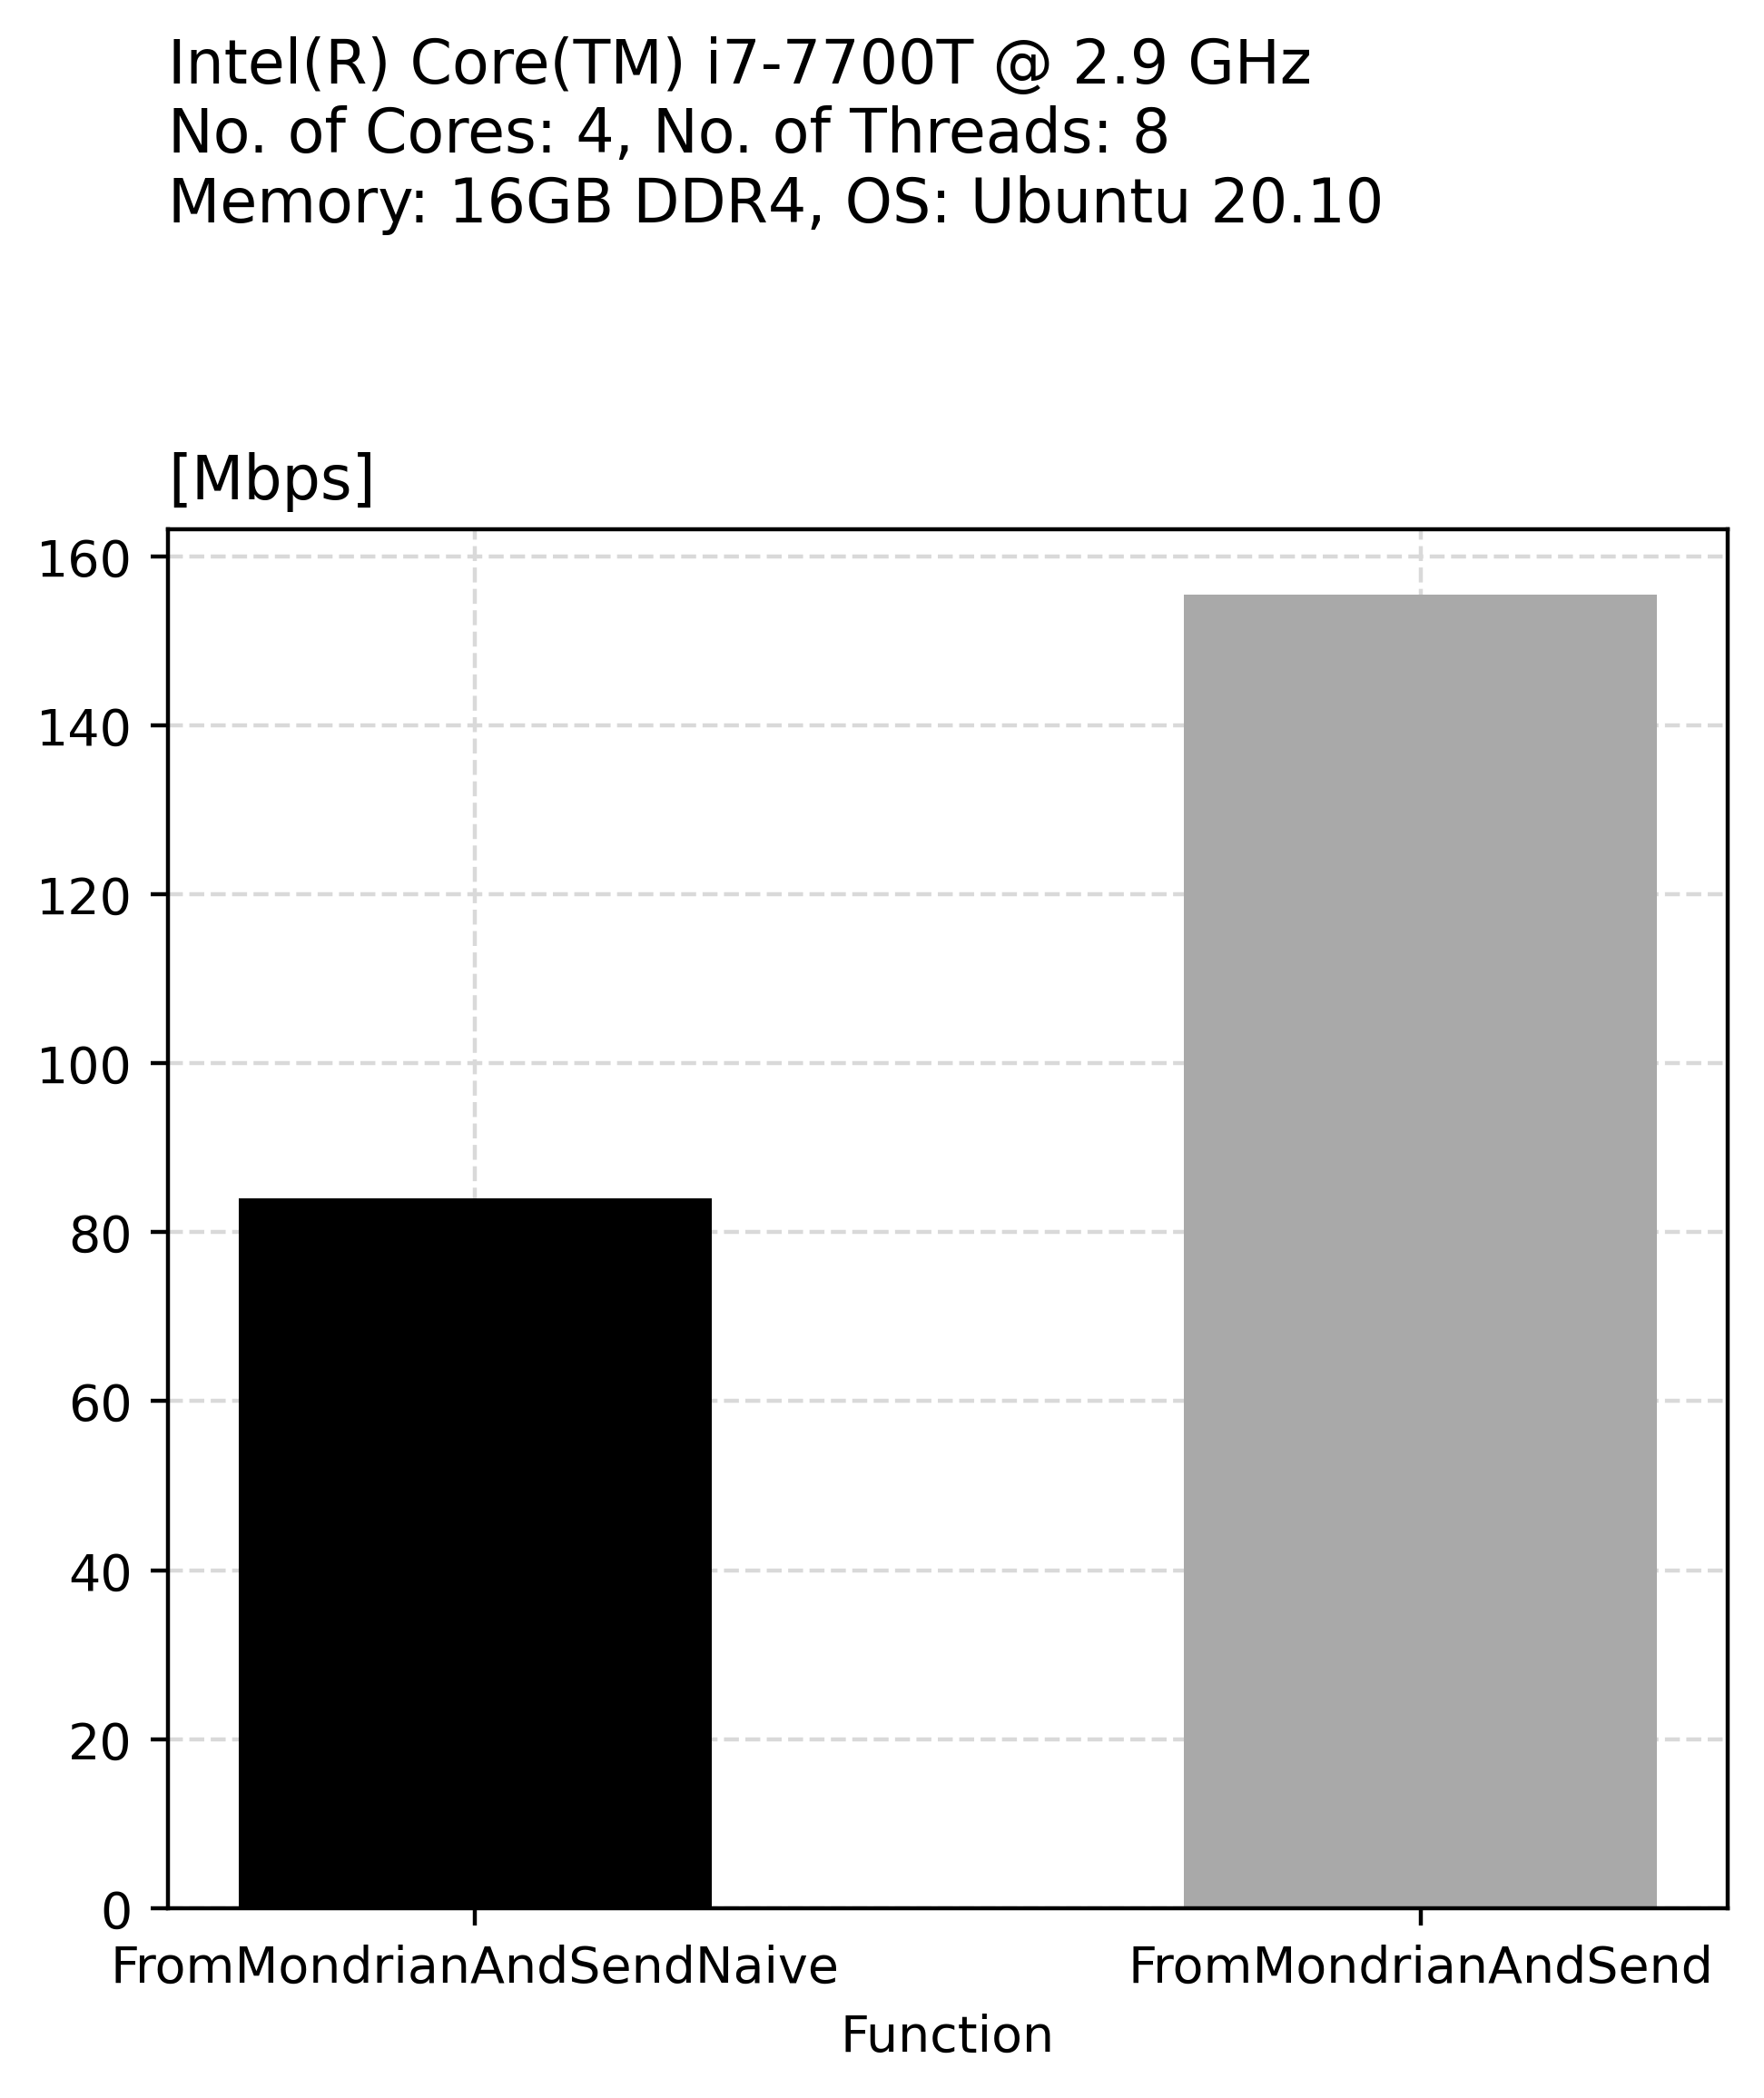
\includegraphics[width=\linewidth]{img/from_mondrian_and_send_opt_throughput.png}
      \caption{Throughput Improvement}
      \label{fig:sub2: Throughput Improvement}
    \end{subfigure}
    \caption{Microbenchmarking Results of the Performance Improvement in \texttt{FromMondrianAndSend} (thanks to \texttt{gopacket} related optimizations)}
    \label{fig:Performance Improvement in FromMondrianAndSend}
\end{figure}

% \clearpage
% \newpage
% \FloatBarrier
\subsection{Security Evaluation}\label{Security Evaluation}
\subsubsection{Threat Agents}\label{Threat Agents}
While there exist countless threat agents, few of them are of particular importance in the context of inter-domain network zoning in data centers.
\paragraph{Nation State Actors} As more and more important data from the private as well as from the public sector is migrated into the cloud, nation state actors have an increasing interest in spying on traffic between and within data centers. Espionage or sabotage operations are carried out in order to keep a competitive edge over rivaling powers.

\paragraph{Internet Service Providers} Many \acsp{ISP} (\aclp{ISP}) are partially or completely owned by nations. This means that they can't be trusted whenever the country in which they are based isn't trustworthy. Furthermore, \acsp{ISP} have monetary interests and might want to sniff on traffic to gain money through targeted advertising.

\paragraph{Competing Customers} Since data centers are multi tenancy environments, different customers of a data center might be competing companies. It therefore must be assumed that a host has an incentive to attack a different host of the same data center.  


\paragraph{Cyber Criminals} Just like any other computer network, data centers are targets of cyber criminals with monetary interests. Lots of valuable data is stored in data centers and the networks are usually enormous. It is therefore crucial, to provide a rigorous zoning mechanism to prevent lateral movement, originating from compromised hosts

%\todo{\\
%    - Many in general but some noteworthy\\
%    - Nation state adversary controling an ISP -- major reason why some sectors hesitate to move into a hybrid cloud model \\
%    - Competition which might try to compromise the availability of a competing service (can buy hosts in the same DC -- multy tenant environment)
%}
\subsubsection{Assets}
In the following subsections, we will discuss some of the most important assets we have to consider when doing our security evaluation. The intention is not to provide a full list of assets, but instead to focus on the most relevant ones. We group the assets into three different categories. Physical assets like physical machines, logical assets like software and information and finally intangible assets like confidentiality, integrity and availability (CIA triad).
\paragraph{Physical Assets}
Physical assets that we must take into consideration are the physical machines hosting the Gateway \acsp{TP}, the Endpoint \acsp{TP} together with the \acs{SDN} controller and the MONDRIAN Controller as well as the servers hosting the clients. The advantage of a data center and its heavily virtualized nature is that all these physical servers will most likely be the same or at least similar. Therefore, we just have to follow data center operator's best practices for providing safety and security for these physical assets. 
%\todo{Gateway TP Server, Endpoint TP Server/SDN controller, MONDRIAN Controller, Host machines}
\paragraph{Logical Assets}
Software wise, the most important asset we must consider is the entire software stack we utilize for the implementation of the MONDRIAN software portfolio. This includes the security of the programming languages, frameworks and libraries that we used, as well as the \acs{SDN} controller, the OpenFlow protocol and the \acs{SDN} switches. Since \acs{SDN} is heavily used in modern data centers, we should use the technologies that are already in place, since they have proven to be reliable and are well maintained, which improves the security of the overall system.

Regarding information assets, we must consider data at rest, as well as in transit. Data at rest is shielded from unauthorized access thanks to MONDRIAN's zone isolation properties. Data in transit consists of control plane traffic and data plane traffic. Control plane traffic is secured by using state of the art encryption protocols. In our case it is \acs{TLS}, but it could be any other protocol that might come up in the future. Inter-domain data plane traffic is encrypted and authenticated by using standard \acs{AES} encryption in \acs{GCM} mode. Additionally, we also have to consider the security of keys and certificates. We assume that the certificates are provided via a secure \acs{PKI}, which is already in place in modern data centers. Symmetric keys are dynamically created according to the \acs{DRKey} derivation scheme, which is also used in other protocols and is believed to be secure.
%\todo{Software of MONDRIAN software portfolio, SDN Controller + Openflow protocol+switches, information: Data at rest and in transit}
\paragraph{Intangible Assets}
The intangible assets we need to take into consideration are confidentiality and integrity of inter-domain traffic, isolation between different MONDRIAN zones as well as the availability of both intra- and inter-domain traffic. Confidentiality and integrity of inter-domain traffic is provided by using an \acs{AEAD}, which is based on \acs{AES} in \acs{GCM} mode. Isolation between MONDRIAN zones is provided if MONDRIAN is deployed correctly, meaning that the order of the \acs{SFC} is respected and all relevant switches are connected to an Endpoint \acs{TP}. The availability of services in a data center that is using MONDRIAN could be compromised in case of a \acs{DDoS} (\acl{DDoS}) attack. We will discuss that further in sections \ref{Security Improvements} and \ref{New Attack Vectors}.
%\todo{Confidentiality + authenticity of inter domain traffic, isolation of zones, availability of intra and inter domain traffic}

\subsubsection{Attacker Model}
As we discussed in section \ref{Threat Agents}, nation state actors as well as \acsp{ISP} are amongst the relevant threat agents. It therefore must be assumed that the entire inter-domain network, whether it is the public internet or an \acs{MPLS} (\acl{MPLS}) network doesn't make a huge difference, is not trustworthy and might be under the adversary's control. This means that we consider a standard Dolev-Yao attacker on the inter-domain network.

Furthermore, we saw in section \ref{Threat Agents} that the customers of a data center can't trust each other. This means that on the internal network we assume to have zones with compromised hosts, which completely control the virtual machine but can't compromise any networking components or the hypervisor.

Finally we assume to have perfect cryptography, meaning that encryptions can't be broken and signatures and \acsp{MAC} can't be forged.

%\todo{\\
%    - Dolev-Yao on the network \\
%    - Malitious customers (compromised hosts) \\
%    - Perfect Crypto \\
%}
\subsubsection{Security Improvements}\label{Security Improvements}
When comparing the new MONDRIAN design with the original one, there are two main security improvements that come with the new design. 

Firstly, the design of the Gateway \acs{TP} is much leaner than the one of the \acs{TP} from the original MONDRIAN design. This has the advantage that the attack surface is reduced, which is particularly important for the Gateway \acs{TP} due to its exposure to the public internet. If an attacker (either from the inside or outside of the data center) tries to compromise the availability of the data center by mounting a volumetric \acs{DDoS} attack on the system, it is an advantage to have a more performant Gateway \acs{TP}. Furthermore, not being in charge of performing zone transition authorization also means that no state needs to be kept. This improves the scalability of a Gateway \acs{TP} compared to the one of a traditional \acs{TP}, which in turn again makes the system more resilient to volumetric \acs{DDoS} attacks, since new instances of Gateway \acsp{TP} could be started up in a matter of seconds.

Secondly, the original MONDRIAN design does not provide egress filtering within the local domain. While unauthorized traffic is prevented from traversing the inter-domain connections, it could still cause congestion in the local network when it is routed to the \acs{TP}. In the new design, unauthorized traffic gets blocked at the first \acs{SDN} switch, which is connected to an Endpoint \acs{TP}, which is usually the virtual switch of the hypervisor. This prevents unauthorized traffic from using bandwidth in the data center's network and therefore reduces the risk of a volumetric DDoS attack of a host targeting the data center's network.

%\todo{\\
%    - Simpler Gateway TP reduces attack surface from the outside world\\
%    - Egress filtering right at the hypervisor prevents network congestion 
%    in the DC network fabric and prevents unauthorized traffic from using costly bandwidth 
%    (especially over expensive leased lines)
%}
\subsubsection{New Attack Vectors}\label{New Attack Vectors}
The new MONDRIAN design provides the same security properties regarding confidentiality, integrity and end-host anonymity of inter-domain traffic as the original MONDRIAN design. It also provides the same level of zone isolation, which means that new attack vectors can mainly be found when analyzing the new \acs{SDN} based design principles and their effect on the availability of the system. 

An attacker controlling a host in a data center could try to mount a \acs{DDoS} attack on the MONDRIAN deployment, by artificially crafting traffic that generates a maximum number of packet-in messages. Such a traffic pattern could for example be traffic, where each packet has a different source port. In that case, each packet would cause a flow table miss and trigger a packet-in message. A different candidate for a malicious traffic pattern would be replies to a connection, which hasn't been initialized but would be allowed, due to an established rule, if it had been initialized. Such packets can't be blocked on the \acs{SDN} switches since it's the Endpoint \acs{TP}'s responsibility to check in the connection state if such a connection has been initialized.

The first attack could be mitigated by simply deciding to not check certain properties. It is questionable, if a data center operator even needs to enforce policies based on the source port, since they are often chosen arbitrarily. If the operator decides not to check the source port then it should be possible to omit that check.

For the second attack vector, a mitigation technique would be to be more thoughtful in the policy making process. If the destination of a policy with \textit{established} as an action is trustworthy and won't mount such an attack, then such a policy will not cause any problems. However, for untrusted zones, established policies with these zones as destination zones should be avoided.

Note that both attacks can easily be detected, by logging and analyzing packet-in messages on the Endpoint \acs{TP} and could alert an administrator, which could then take the aforementioned countermeasures if desired.

%\todo{\\
%    - specially crafted traffic could cause many packet-in messages and DDoS the Endpoint TP\\
%    - Unwise policy decissions can increase the workload on the Endpoint TPs (wildcards 
%    should be avoided -- in some situations not checking some fields might make sense (srcPort))
%}

\section{Discussion}
\label{sec:discussion}
% \chapter{Discussion}
Now that we have shown the feasibility of the new MONDRIAN design, there are still some practical considerations we need to discuss. We will discuss the deployability of MONDRIAN in a real-world scenario and examine what needs to be thought of regarding the placement of components and the creation of redundant instances to increase scalability and robustness.

\subsection{Deployment}
For MONDRIAN to find its way into a production environment, it is not sufficient to just prove that the functionality, security and performance requirements are met. There are some practical issues that we need to consider. A very important one is the deployability of the architecture. Hyperscale data centers like the ones of public cloud providers are extremely big and therefore very costly. Therefore, making changes to the infrastructure, happens very carefully and incrementally since any downtime can quickly become expensive. In the following subsections, we will discuss the incremental deployability of MONDRIAN, how a partial deployment could already be beneficial and what a nested deployment model would look like.

\subsubsection{Incremental Deployability} \label{Incremental Deployability}
A significant benefit regarding incremental deployability of the new MONDRIAN design is that since the tunneling mechanism a Gateway \acs{TP} provides is separated from the zone transition authorization mechanism an Endpoint \acs{TP} provides, we can deploy the two components separately.

We could start by deploying a Gateway \acs{TP} at each site. If a Gateway \acs{TP} doesn't know how to handle some kind of traffic, for example, because the zones have not yet been registered in the MONDRIAN Controller, it simply forwards the \acs{IP} traffic without modifying it. We could therefore route all traffic that doesn't contain a MONDRIAN header through the legacy tunneling middlebox, which would most likely be a \acs{VPN} endpoint (see figure \ref{Gateway TP Use Case for Incremental Deployment}). As we keep adding zone information to the MONDRIAN Controller, more and more output traffic of a Gateway \acs{TP} will be MONDRIAN traffic and at some point, the legacy tunneling mechanism will become obsolete.

\begin{figure}[t]
	\centering
	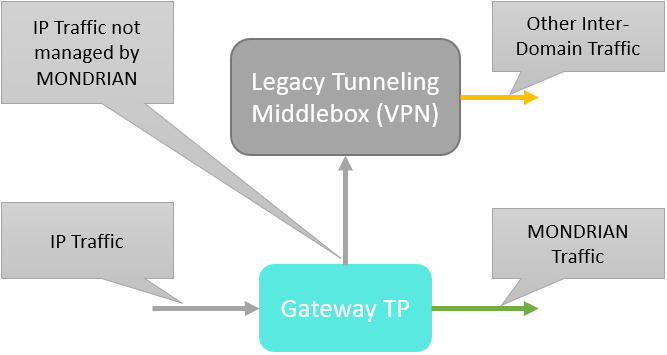
\includegraphics[width =.48\textwidth]{img/Gateway_TP_partial_incremental_deployment.png}
	\caption{Temporary Gateway \acs{TP} Use Case for Incremental Deployment (for as long as not all traffic is managed by MONDRIAN)}
	\label{Gateway TP Use Case for Incremental Deployment}
\end{figure}
\FloatBarrier
When deploying Endpoint \acsp{TP}, we need to specify what to do with traffic that isn't managed by MONDRIAN. The easiest way to do that is to create one huge zone, which at first contains all hosts. We refer to this zone as the \textit{Legacy Zone}, since within this zone a non-MONDRIAN architecture is responsible for implementing a zoning mechanism. At first, we will have only intra-zone traffic within the \textit{Legacy Zone}. Then we can start moving hosts into newly created zones and specify the desired zone transition policies. At first, we might want to have a policy, which allows all traffic from the \textit{Legacy Zone} to the newly created zone as well as one in the opposite direction (see the first two policies in \ref{Legacy Policy}). Once we are confident that the new policies reflect the desired behavior, we can change these two policies such that they drop traffic between the new zone and the \textit{Legacy Zone} (see the last two policies in \ref{Legacy Policy}). Once the \textit{Legacy Zone} is empty, we can remove it from MONDRIAN as well as all the policies associated with it. At this point, the migration to MONDRIAN will be complete, without having ever experienced any major downtimes in the process.

\begin{align}\label{Legacy Policy}
    \nonumber \text{Legacy Zone} &= \{0.0.0.0/0\}\\
    \nonumber <\text{Legacy Zone}, *, \text{Zone 1}, *, *>&\Rightarrow <forwarding>\\
    <\text{Zone 1}, *, \text{Legacy Zone}, *, *>&\Rightarrow <forwarding>\\
    \nonumber <\text{Legacy Zone}, *, \text{Zone 2}, *, *>&\Rightarrow <drop>\\
    \nonumber <\text{Zone 2}, *, \text{Legacy Zone}, *, *>&\Rightarrow <drop>
\end{align}

\subsubsection{Partial Deployability}
In large data centers, it might be that there are some customers, for which MONDRIAN is not suitable (for example due to regulatory issues) or data center operators might want to test out MONDRIAN on a subset of their infrastructure and see if the benefits are worth the investment. For such scenarios, it should be possible to use MONDRIAN in a partial deployment.

Partial deployment of MONDRIAN is of course possible without any complications. We could simply follow the deployment process described in section \ref{Incremental Deployability} and leave the parts of the infrastructure that we don't want to manage using MONDRIAN in the \textit{Legacy Zone}.

Such a partial deployment scenario could make sense if there are parts of the infrastructure where enforcing zone transition policies based on the 5-tuplet of a MONDRIAN rule is not enough, but instead deep packet inspection is required. The data center operators could employ these more advanced checks by using other technologies while still benefiting from the simplified manageability MONDRIAN provides to manage the parts of the network, where checking the 5-tuplet from the MONDRIAN rules is sufficient.

\subsubsection{Nested Deployment Models}

Until now, we only considered the use case, where data center operators use MONDRIAN. However, the customers of a public cloud provider might also want to create their own zones within the zone, which has been assigned to them by the data center operators. The customers will require control over their custom zones and want to define their own policies, without the oversight of a data center operator. 

They might already have MONDRIAN in use for managing the zone transitions in their corporate network. When transitioning into a hybrid cloud model, they would most likely want to employ MONDRIAN in their cloud as well. However, customers of cloud providers usually have no control over the networking mechanisms employed in the cloud provider's data center. This makes the new MONDRIAN design unsuitable for the customers. However, it is still perfectly possible to deploy a traditional MONDRIAN \acs{TP} into a \acs{VM} in the cloud and set this \acs{VM} as the default gateway for all other hosts in the cloud. 

Currently, we typically have \acs{VPN} endpoints on host machines in the cloud, which act as a default gateway and create a tunnel between the cloud and the corporate network. This \acs{VPN} endpoint could simply be replaced with a MONDRIAN \acs{TP} and then the customer would be free to use his own MONDRIAN deployment, regardless of the network zoning architecture the data center operators employ. This also shows that the original MONDRIAN design will not be replaced by the new one but instead both versions will be used, wherever they fit best.

\FloatBarrier
\subsection{Component Placement and Redundancy}
As we already discussed in section \ref{Performance Evaluation}, both the Endpoint \acs{TP} as well as the Gateway \acs{TP} are highly scalable due to their almost stateless nature (the only states are the connection states of the Endpoint \acsp{TP}, which don't need to be synchronized between different instances). This means that we should have multiple instances of Gateway \acsp{TP} and Endpoint \acsp{TP} to increase robustness thanks to redundancy and to allow for fast failover of single instances, as well as balance the workload individual instances experience.

The MONDRIAN Controller is basically a database server. It is therefore clear that multiple instances need to be synchronized amongst each other. However, this doesn't pose a problem, since the databases of MONDRIAN Controllers are read-heavy. A simple Master-Slave synchronization strategy will be sufficient for synchronizing multiple instances. One MONDRIAN Controller would be the master node, where the administrator would directly change the configurations. The other MONDRIAN Controllers would be slave nodes, which would ideally be located at the individual sites to minimize the latency between the different \acsp{TP} and the MONDRIAN Controller during the fetching process. Furthermore, placing instances of MONDRIAN Controllers at each site would ensure reachability even if the internet connection is unreliable during the fetching period. Depending on the size of the data center and consequently the number of Endpoint \acsp{TP} and Gateway \acsp{TP} per site, it could even make sense to have multiple instances of a  MONDRIAN Controller per site to balance the workload.

%\todo{\\
%    - Incremental deployability\\
%    - Partial deployments\\
%    - Nested deplyoment (hybrid cloud customers)\\
%    - Placement and redundancy of controller
%}

\section{Related Work}
\label{sec:related_work}
% \chapter{Related Work}

The most important paper related to this thesis is of course the original MONDRIAN paper, proposing the original design of MONDRIAN \cite{kwonmondrian}. It introduced many concepts, which have been reused in this thesis, such as the concept of a MONDRIAN Controller working together with different \acsp{TP}, which are located at different sites. It further specifies the functionality of the Authentication Module, as well as the Transition Module. Using the \acs{DRKey} derivation scheme for establishing shared secrets between \acsp{TP} is an idea, which has been borrowed from the aforementioned paper. 

What modern data centers look like and what concepts exist in the field of \acs{SDDC} (\acl{SDDC}) is discussed in a whitepaper about VMware\texttrademark's NSX data center platform \cite{vmware2021nsx}. The concept of virtual distributed switches, like they can be found in VMware's products, served as an inspiration for the distributed nature of the Endpoint \acs{TP}. Current research questions concerning cloud data centers and where in data centers high costs occur and what the challenges are to minimize them is discussed in the paper \textit{"The Cost of a Cloud: Research Problems in Data Center Networks"} \cite{greenberg2008cost}. This paper also highlights the importance of saving bandwidth, both in the inter-domain as well as in the intra-domain case. The Endpoint \acs{TP} addresses this problem by providing a more advanced egress-filtering mechanism than the original \acs{TP}.

Regarding \acs{SDN}, there is a paper written by Intel\texttrademark,  discussing how a \acs{DPDK} enabled \acs{OVS} can enable \acs{SDN} and \acs{NFV} transformation \cite{intel2015OVS}. It shows the performance gains \acs{OVS} achieves thanks to the use of \acs{DPDK} and how the \acs{OVS} integrates seamlessly into the \acs{NFV} reference architecture, proposed by the \acs{ETSI}. A great overview over the numerous northbound interfaces that exist for \acs{SDN} is provided by a paper called \textit{"The Northbound APIs of Software Defined Networks"} \cite{tijare2016northbound}. It shows the important differences between \acs{REST}full and non-\acs{REST}full interfaces of \acs{SDN} controllers and was helpful for deciding which \acs{SDN} controller suites our needs best. Numerous other \acs{SDN} related concepts are described in a book called \textit{"Software Defined Networks"} by Paul Goransson and Chuck Black \cite{goransson2014SDN}. It contains an OpenFlow specification, discusses how \acs{SDN} is used in data centers and other environments and shows example applications based on \acs{SDN}.

In the field of \acs{NFV} there exists a paper highlighting the benefits, enablers and challenges for \acs{NFV} \cite{att2012NFV}. This paper is a collaborative work of many major \acs{Telco} companies and has been presented at the \textit{\acs{SDN} and OpenFlow World Congress}. It provides us with a holistic view over the general state of \acs{NFV} and shows in which direction the entire industry is evolving according to major \acs{Telco} companies.



%\todo{ \\
%	- original mondrian paper \cite{kwonmondrian}\\
%	- what DCs look like \cite{vmware2021nsx}\\
%	- what is important in DCs \cite{greenberg2008cost}\\
%	- OVS for SDN based NFV with DPDK \cite{intel2015OVS}\\
%	- Northbound APIs \cite{tijare2016northbound}\\
%	- Basics about SDN \cite{goransson2014SDN}\\
%	- NFV \cite{att2012NFV}
%}

\section{Conclusion}
\label{sec:conclusion}
% \chapter{Conclusion}

This master thesis project has shown that a modern network zoning architecture like MONDRIAN is also realizable in the context of data center networking. The \acs{PoC} \cite{meinen2021DCMONDRIAN} implementation shows satisfying results and has proven the feasibility of the new MONDRIAN design.

The new MONDRIAN design fully incorporates the concept of \acs{NFV} by providing a hybrid solution, consisting of a traditional \acs{VM}/container-based \acs{VNF} as well as a more modern \acs{SDN} based \acs{VNF}. It follows the design principles that can be found in modern data centers and hence integrates seamlessly into the infrastructure found in data centers.

Even though the current implementation is just a proof of concept and therefore doesn't provide production level performance, the \acs{PoC} implementation proves that there are no conceptual reasons why a highly performant production level implementation could be impossible. All the performance bottlenecks have been identified by rigorously analyzing the \acs{PoC} implementation and can be eliminated by using production level frameworks like \acs{DPDK}.

For data center operators, there exist clear benefits for using a logically centralized inter-domain network zoning architecture like MONDRIAN, mainly because data centers can be enormous in size and due to their multi-tenancy nature, they have very strict network zoning requirements. It is therefore a welcome finding that data center operators can make use of MONDRIAN as well.

The major contributions of this thesis are the introduction of the concept of \aclp{vTP} and the separation of responsibilities of a \acs{TP}, which leads to the introduction of the Gateway \acs{TP} as well as the Endpoint \acs{TP}. Furthermore, the \acs{SDN} based design of the Endpoint \acs{TP} is what distinguishes the new MONDRIAN design the most from the original one and is the major reason why MONDRIAN can now be used in data centers.

%\todo{\\
%    - It works\\
%    - It can be implemented in a performant way (just not with gopackets but DPDK instead)\\
%    - Clear benefits exist for DC Operators\\
%    - Major contribution of this Thesis: SDN approach for Endpoint TPs, concept of vTP = Gateway TP + Endpoint TP
%}

\bibliographystyle{IEEEtranS}
\bibliography{refs}

% \begin{thebibliography}{00}
% \bibitem{b1} G. Eason, B. Noble, and I. N. Sneddon, ``On certain integrals of Lipschitz-Hankel type involving products of Bessel functions,'' Phil. Trans. Roy. Soc. London, vol. A247, pp. 529--551, April 1955.
% \bibitem{b2} J. Clerk Maxwell, A Treatise on Electricity and Magnetism, 3rd ed., vol. 2. Oxford: Clarendon, 1892, pp.68--73.
% \bibitem{b3} I. S. Jacobs and C. P. Bean, ``Fine particles, thin films and exchange anisotropy,'' in Magnetism, vol. III, G. T. Rado and H. Suhl, Eds. New York: Academic, 1963, pp. 271--350.
% \bibitem{b4} K. Elissa, ``Title of paper if known,'' unpublished.
% \bibitem{b5} R. Nicole, ``Title of paper with only first word capitalized,'' J. Name Stand. Abbrev., in press.
% \bibitem{b6} Y. Yorozu, M. Hirano, K. Oka, and Y. Tagawa, ``Electron spectroscopy studies on magneto-optical media and plastic substrate interface,'' IEEE Transl. J. Magn. Japan, vol. 2, pp. 740--741, August 1987 [Digests 9th Annual Conf. Magnetics Japan, p. 301, 1982].
% \bibitem{b7} M. Young, The Technical Writer's Handbook. Mill Valley, CA: University Science, 1989.
% \end{thebibliography}
% \vspace{12pt}
% \color{red}
% IEEE conference templates contain guidance text for composing and formatting conference papers. Please ensure that all template text is removed from your conference paper prior to submission to the conference. Failure to remove the template text from your paper may result in your paper not being published.

\end{document}
